\documentclass[twoside]{book}

% Packages required by doxygen
\usepackage{fixltx2e}
\usepackage{calc}
\usepackage{doxygen}
\usepackage[export]{adjustbox} % also loads graphicx
\usepackage{graphicx}
\usepackage[utf8]{inputenc}
\usepackage{makeidx}
\usepackage{multicol}
\usepackage{multirow}
\PassOptionsToPackage{warn}{textcomp}
\usepackage{textcomp}
\usepackage[nointegrals]{wasysym}
\usepackage[table]{xcolor}

% Font selection
\usepackage[T1]{fontenc}
\usepackage[scaled=.90]{helvet}
\usepackage{courier}
\usepackage{amssymb}
\usepackage{sectsty}
\renewcommand{\familydefault}{\sfdefault}
\allsectionsfont{%
  \fontseries{bc}\selectfont%
  \color{darkgray}%
}
\renewcommand{\DoxyLabelFont}{%
  \fontseries{bc}\selectfont%
  \color{darkgray}%
}
\newcommand{\+}{\discretionary{\mbox{\scriptsize$\hookleftarrow$}}{}{}}

% Page & text layout
\usepackage{geometry}
\geometry{%
  a4paper,%
  top=2.5cm,%
  bottom=2.5cm,%
  left=2.5cm,%
  right=2.5cm%
}
\tolerance=750
\hfuzz=15pt
\hbadness=750
\setlength{\emergencystretch}{15pt}
\setlength{\parindent}{0cm}
\setlength{\parskip}{3ex plus 2ex minus 2ex}
\makeatletter
\renewcommand{\paragraph}{%
  \@startsection{paragraph}{4}{0ex}{-1.0ex}{1.0ex}{%
    \normalfont\normalsize\bfseries\SS@parafont%
  }%
}
\renewcommand{\subparagraph}{%
  \@startsection{subparagraph}{5}{0ex}{-1.0ex}{1.0ex}{%
    \normalfont\normalsize\bfseries\SS@subparafont%
  }%
}
\makeatother

% Headers & footers
\usepackage{fancyhdr}
\pagestyle{fancyplain}
\fancyhead[LE]{\fancyplain{}{\bfseries\thepage}}
\fancyhead[CE]{\fancyplain{}{}}
\fancyhead[RE]{\fancyplain{}{\bfseries\leftmark}}
\fancyhead[LO]{\fancyplain{}{\bfseries\rightmark}}
\fancyhead[CO]{\fancyplain{}{}}
\fancyhead[RO]{\fancyplain{}{\bfseries\thepage}}
\fancyfoot[LE]{\fancyplain{}{}}
\fancyfoot[CE]{\fancyplain{}{}}
\fancyfoot[RE]{\fancyplain{}{\bfseries\scriptsize Generated by Doxygen }}
\fancyfoot[LO]{\fancyplain{}{\bfseries\scriptsize Generated by Doxygen }}
\fancyfoot[CO]{\fancyplain{}{}}
\fancyfoot[RO]{\fancyplain{}{}}
\renewcommand{\footrulewidth}{0.4pt}
\renewcommand{\chaptermark}[1]{%
  \markboth{#1}{}%
}
\renewcommand{\sectionmark}[1]{%
  \markright{\thesection\ #1}%
}

% Indices & bibliography
\usepackage{natbib}
\usepackage[titles]{tocloft}
\setcounter{tocdepth}{3}
\setcounter{secnumdepth}{5}
\makeindex

% Hyperlinks (required, but should be loaded last)
\usepackage{ifpdf}
\ifpdf
  \usepackage[pdftex,pagebackref=true]{hyperref}
\else
  \usepackage[ps2pdf,pagebackref=true]{hyperref}
\fi
\hypersetup{%
  colorlinks=true,%
  linkcolor=blue,%
  citecolor=blue,%
  unicode%
}

% Custom commands
\newcommand{\clearemptydoublepage}{%
  \newpage{\pagestyle{empty}\cleardoublepage}%
}

\usepackage{caption}
\captionsetup{labelsep=space,justification=centering,font={bf},singlelinecheck=off,skip=4pt,position=top}

%===== C O N T E N T S =====

\begin{document}

% Titlepage & ToC
\hypersetup{pageanchor=false,
             bookmarksnumbered=true,
             pdfencoding=unicode
            }
\pagenumbering{alph}
\begin{titlepage}
\vspace*{7cm}
\begin{center}%
{\Large Share It \\[1ex]\large v 2.\+0 }\\
\vspace*{1cm}
{\large Generated by Doxygen 1.8.13}\\
\end{center}
\end{titlepage}
\clearemptydoublepage
\pagenumbering{roman}
\tableofcontents
\clearemptydoublepage
\pagenumbering{arabic}
\hypersetup{pageanchor=true}

%--- Begin generated contents ---
\chapter{Module Index}
\section{Modules}
Here is a list of all modules\+:\begin{DoxyCompactList}
\item \contentsline{section}{Agency}{\pageref{group___agency}}{}
\item \contentsline{section}{Candidate\+Trip}{\pageref{group___candidate_trip}}{}
\item \contentsline{section}{Date}{\pageref{group___date}}{}
\item \contentsline{section}{Hour}{\pageref{group___hour}}{}
\item \contentsline{section}{Functions}{\pageref{group___template}}{}
\item \contentsline{section}{Stop}{\pageref{group___stop}}{}
\item \contentsline{section}{Tools}{\pageref{group___tools}}{}
\item \contentsline{section}{Transaction}{\pageref{group___transaction}}{}
\item \contentsline{section}{Trip}{\pageref{group___trip}}{}
\item \contentsline{section}{User}{\pageref{group___user}}{}
\item \contentsline{section}{Utilities}{\pageref{group___utilities}}{}
\item \contentsline{section}{Vehicle}{\pageref{group___vehicle}}{}
\end{DoxyCompactList}

\chapter{Hierarchical Index}
\section{Class Hierarchy}
This inheritance list is sorted roughly, but not completely, alphabetically\+:\begin{DoxyCompactList}
\item \contentsline{section}{Agency}{\pageref{class_agency}}{}
\item \contentsline{section}{Binary\+Node$<$ Comparable $>$}{\pageref{class_binary_node}}{}
\item \contentsline{section}{Binary\+Node$<$ Vehicle $>$}{\pageref{class_binary_node}}{}
\item \contentsline{section}{B\+ST$<$ Comparable $>$}{\pageref{class_b_s_t}}{}
\item \contentsline{section}{B\+ST$<$ Vehicle $>$}{\pageref{class_b_s_t}}{}
\item \contentsline{section}{B\+S\+T\+Itr\+In$<$ Comparable $>$}{\pageref{class_b_s_t_itr_in}}{}
\item \contentsline{section}{B\+S\+T\+Itr\+Level$<$ Comparable $>$}{\pageref{class_b_s_t_itr_level}}{}
\item \contentsline{section}{B\+S\+T\+Itr\+Post$<$ Comparable $>$}{\pageref{class_b_s_t_itr_post}}{}
\item \contentsline{section}{B\+S\+T\+Itr\+Pre$<$ Comparable $>$}{\pageref{class_b_s_t_itr_pre}}{}
\item \contentsline{section}{Candidate\+Trip}{\pageref{class_candidate_trip}}{}
\item \contentsline{section}{cars}{\pageref{structcars}}{}
\item \contentsline{section}{Date}{\pageref{class_date}}{}
\item \contentsline{section}{distance\+Struct}{\pageref{structdistance_struct}}{}
\item \contentsline{section}{Error}{\pageref{class_error}}{}
\item \contentsline{section}{Hour}{\pageref{class_hour}}{}
\item \contentsline{section}{inactive\+Ptr}{\pageref{structinactive_ptr}}{}
\item \contentsline{section}{Invalid\+Date}{\pageref{class_invalid_date}}{}
\item \contentsline{section}{Invalid\+Hour}{\pageref{class_invalid_hour}}{}
\item \contentsline{section}{Nonexistent\+Car}{\pageref{class_nonexistent_car}}{}
\item \contentsline{section}{Nonexistent\+Stop}{\pageref{class_nonexistent_stop}}{}
\item \contentsline{section}{Passed\+Date}{\pageref{class_passed_date}}{}
\item \contentsline{section}{Passed\+Hour}{\pageref{class_passed_hour}}{}
\item \contentsline{section}{Repeated\+Stop}{\pageref{class_repeated_stop}}{}
\item \contentsline{section}{stop}{\pageref{structstop}}{}
\item \contentsline{section}{Stop}{\pageref{class_stop}}{}
\item \contentsline{section}{Too\+Long}{\pageref{class_too_long}}{}
\item \contentsline{section}{Transaction}{\pageref{class_transaction}}{}
\item \contentsline{section}{Trip}{\pageref{class_trip}}{}
\item \contentsline{section}{User}{\pageref{class_user}}{}
\begin{DoxyCompactList}
\item \contentsline{section}{Driver}{\pageref{class_driver}}{}
\item \contentsline{section}{Passenger}{\pageref{class_passenger}}{}
\end{DoxyCompactList}
\item \contentsline{section}{user\+Gone}{\pageref{classuser_gone}}{}
\item \contentsline{section}{user\+Ptr}{\pageref{structuser_ptr}}{}
\item \contentsline{section}{Vehicle}{\pageref{class_vehicle}}{}
\end{DoxyCompactList}

\chapter{Class Index}
\section{Class List}
Here are the classes, structs, unions and interfaces with brief descriptions\+:\begin{DoxyCompactList}
\item\contentsline{section}{\hyperlink{class_agency}{Agency} }{\pageref{class_agency}}{}
\item\contentsline{section}{\hyperlink{class_binary_node}{Binary\+Node$<$ Comparable $>$} }{\pageref{class_binary_node}}{}
\item\contentsline{section}{\hyperlink{class_b_s_t}{B\+S\+T$<$ Comparable $>$} }{\pageref{class_b_s_t}}{}
\item\contentsline{section}{\hyperlink{class_b_s_t_itr_in}{B\+S\+T\+Itr\+In$<$ Comparable $>$} }{\pageref{class_b_s_t_itr_in}}{}
\item\contentsline{section}{\hyperlink{class_b_s_t_itr_level}{B\+S\+T\+Itr\+Level$<$ Comparable $>$} }{\pageref{class_b_s_t_itr_level}}{}
\item\contentsline{section}{\hyperlink{class_b_s_t_itr_post}{B\+S\+T\+Itr\+Post$<$ Comparable $>$} }{\pageref{class_b_s_t_itr_post}}{}
\item\contentsline{section}{\hyperlink{class_b_s_t_itr_pre}{B\+S\+T\+Itr\+Pre$<$ Comparable $>$} }{\pageref{class_b_s_t_itr_pre}}{}
\item\contentsline{section}{\hyperlink{class_candidate_trip}{Candidate\+Trip} }{\pageref{class_candidate_trip}}{}
\item\contentsline{section}{\hyperlink{structcars}{cars} }{\pageref{structcars}}{}
\item\contentsline{section}{\hyperlink{class_date}{Date} }{\pageref{class_date}}{}
\item\contentsline{section}{\hyperlink{structdistance_struct}{distance\+Struct} }{\pageref{structdistance_struct}}{}
\item\contentsline{section}{\hyperlink{class_driver}{Driver} }{\pageref{class_driver}}{}
\item\contentsline{section}{\hyperlink{class_error}{Error} }{\pageref{class_error}}{}
\item\contentsline{section}{\hyperlink{class_hour}{Hour} }{\pageref{class_hour}}{}
\item\contentsline{section}{\hyperlink{structinactive_ptr}{inactive\+Ptr} }{\pageref{structinactive_ptr}}{}
\item\contentsline{section}{\hyperlink{class_invalid_date}{Invalid\+Date} }{\pageref{class_invalid_date}}{}
\item\contentsline{section}{\hyperlink{class_invalid_hour}{Invalid\+Hour} }{\pageref{class_invalid_hour}}{}
\item\contentsline{section}{\hyperlink{class_nonexistent_car}{Nonexistent\+Car} }{\pageref{class_nonexistent_car}}{}
\item\contentsline{section}{\hyperlink{class_nonexistent_stop}{Nonexistent\+Stop} }{\pageref{class_nonexistent_stop}}{}
\item\contentsline{section}{\hyperlink{class_passed_date}{Passed\+Date} }{\pageref{class_passed_date}}{}
\item\contentsline{section}{\hyperlink{class_passed_hour}{Passed\+Hour} }{\pageref{class_passed_hour}}{}
\item\contentsline{section}{\hyperlink{class_passenger}{Passenger} }{\pageref{class_passenger}}{}
\item\contentsline{section}{\hyperlink{class_repeated_stop}{Repeated\+Stop} }{\pageref{class_repeated_stop}}{}
\item\contentsline{section}{\hyperlink{structstop}{stop} }{\pageref{structstop}}{}
\item\contentsline{section}{\hyperlink{class_stop}{Stop} }{\pageref{class_stop}}{}
\item\contentsline{section}{\hyperlink{class_too_long}{Too\+Long} }{\pageref{class_too_long}}{}
\item\contentsline{section}{\hyperlink{class_transaction}{Transaction} }{\pageref{class_transaction}}{}
\item\contentsline{section}{\hyperlink{class_trip}{Trip} }{\pageref{class_trip}}{}
\item\contentsline{section}{\hyperlink{class_user}{User} }{\pageref{class_user}}{}
\item\contentsline{section}{\hyperlink{classuser_gone}{user\+Gone} }{\pageref{classuser_gone}}{}
\item\contentsline{section}{\hyperlink{structuser_ptr}{user\+Ptr} \\*Struct used for hash insertion }{\pageref{structuser_ptr}}{}
\item\contentsline{section}{\hyperlink{class_vehicle}{Vehicle} }{\pageref{class_vehicle}}{}
\end{DoxyCompactList}

\chapter{Module Documentation}
\hypertarget{group___agency}{}\section{Agency}
\label{group___agency}\index{Agency@{Agency}}
\subsection*{Classes}
\begin{DoxyCompactItemize}
\item 
struct \hyperlink{structstop}{stop}
\item 
struct \hyperlink{structinactive_ptr}{inactive\+Ptr}
\item 
struct \hyperlink{structcars}{cars}
\item 
struct \hyperlink{structdistance_struct}{distance\+Struct}
\item 
class \hyperlink{class_agency}{Agency}
\end{DoxyCompactItemize}
\subsection*{Typedefs}
\begin{DoxyCompactItemize}
\item 
\mbox{\Hypertarget{group___agency_gac4e50fb3eb9c87ffa6e32341378b4af6}\label{group___agency_gac4e50fb3eb9c87ffa6e32341378b4af6}} 
typedef unordered\+\_\+set$<$ \hyperlink{structuser_ptr}{user\+Ptr}, \hyperlink{structinactive_ptr}{inactive\+Ptr}, \hyperlink{structinactive_ptr}{inactive\+Ptr} $>$ {\bfseries tab\+H\+Inactive}
\end{DoxyCompactItemize}
\subsection*{Functions}
\begin{DoxyCompactItemize}
\item 
\mbox{\Hypertarget{group___agency_ga165eb4b729955163f0c52852aa554af1}\label{group___agency_ga165eb4b729955163f0c52852aa554af1}} 
int {\bfseries inactive\+Ptr\+::operator()} (const \hyperlink{structuser_ptr}{user\+Ptr} \&us1) const
\item 
\mbox{\Hypertarget{group___agency_gadc40c7d895103613550bb1c415f849f0}\label{group___agency_gadc40c7d895103613550bb1c415f849f0}} 
bool {\bfseries inactive\+Ptr\+::operator()} (const \hyperlink{structuser_ptr}{user\+Ptr} \&us1, const \hyperlink{structuser_ptr}{user\+Ptr} \&us2) const
\item 
\mbox{\Hypertarget{group___agency_gaf6fc6c4dec00025fce567183f67edbaa}\label{group___agency_gaf6fc6c4dec00025fce567183f67edbaa}} 
\hyperlink{group___agency_gaf6fc6c4dec00025fce567183f67edbaa}{Agency\+::\+Agency} ()
\begin{DoxyCompactList}\small\item\em \hyperlink{class_agency}{Agency} constructor. \end{DoxyCompactList}\item 
\mbox{\Hypertarget{group___agency_ga922750a7051987df9bb697769fdf0256}\label{group___agency_ga922750a7051987df9bb697769fdf0256}} 
\hyperlink{group___agency_ga922750a7051987df9bb697769fdf0256}{Agency\+::$\sim$\+Agency} ()
\begin{DoxyCompactList}\small\item\em \hyperlink{class_agency}{Agency} destructor. \end{DoxyCompactList}\item 
static \hyperlink{class_agency}{Agency} $\ast$ \hyperlink{group___agency_ga573fab41076b962289fad1f14031b68c}{Agency\+::instance} ()
\begin{DoxyCompactList}\small\item\em \hyperlink{class_agency}{Agency} instance creator. \end{DoxyCompactList}\end{DoxyCompactItemize}
\subsection*{Variables}
\begin{DoxyCompactItemize}
\item 
\mbox{\Hypertarget{group___agency_ga79f9fc915ad09783ec07b876d6eed865}\label{group___agency_ga79f9fc915ad09783ec07b876d6eed865}} 
string {\bfseries stop\+::code}
\item 
\mbox{\Hypertarget{group___agency_ga91bd51eb4e3994056d52465dda3a6ca4}\label{group___agency_ga91bd51eb4e3994056d52465dda3a6ca4}} 
string {\bfseries stop\+::name}
\item 
\mbox{\Hypertarget{group___agency_ga604acdb12b949ce28b76c2e0cb29ad81}\label{group___agency_ga604acdb12b949ce28b76c2e0cb29ad81}} 
string {\bfseries cars\+::brand}
\item 
\mbox{\Hypertarget{group___agency_gaf0c7084b7a4fb4ceb5e74330e88d78bb}\label{group___agency_gaf0c7084b7a4fb4ceb5e74330e88d78bb}} 
string {\bfseries cars\+::model}
\item 
\mbox{\Hypertarget{group___agency_gab4158f666bb1f7a8a1ca31f2942ba629}\label{group___agency_gab4158f666bb1f7a8a1ca31f2942ba629}} 
int {\bfseries cars\+::seats}
\item 
\mbox{\Hypertarget{group___agency_gacf7d9670242fa6da94168421f0317c08}\label{group___agency_gacf7d9670242fa6da94168421f0317c08}} 
int {\bfseries cars\+::year}
\item 
\mbox{\Hypertarget{group___agency_ga5fcd18c58d5dd4b65ffb25c6b3f5f088}\label{group___agency_ga5fcd18c58d5dd4b65ffb25c6b3f5f088}} 
int {\bfseries cars\+::available}
\item 
\mbox{\Hypertarget{group___agency_ga2e71e97640f5cc04c32d21c2d3104e06}\label{group___agency_ga2e71e97640f5cc04c32d21c2d3104e06}} 
string {\bfseries distance\+Struct\+::pnt1}
\item 
\mbox{\Hypertarget{group___agency_ga20809a497514156c21cac416a8714971}\label{group___agency_ga20809a497514156c21cac416a8714971}} 
string {\bfseries distance\+Struct\+::pnt2}
\item 
\mbox{\Hypertarget{group___agency_ga41ee5fe344f1b745d3da6986449faa4f}\label{group___agency_ga41ee5fe344f1b745d3da6986449faa4f}} 
float {\bfseries distance\+Struct\+::km}
\item 
\mbox{\Hypertarget{group___agency_ga24c6ae11e29cdf5eefc6a5c94783b90e}\label{group___agency_ga24c6ae11e29cdf5eefc6a5c94783b90e}} 
static \hyperlink{class_agency}{Agency} $\ast$ \hyperlink{group___agency_ga24c6ae11e29cdf5eefc6a5c94783b90e}{Agency\+::singleton\+\_\+instance} = 0
\begin{DoxyCompactList}\small\item\em \hyperlink{class_agency}{Agency} instance. \end{DoxyCompactList}\item 
\mbox{\Hypertarget{group___agency_gadd64fcf15e317225aab8d7e66a113cdd}\label{group___agency_gadd64fcf15e317225aab8d7e66a113cdd}} 
int \hyperlink{group___agency_gadd64fcf15e317225aab8d7e66a113cdd}{Agency\+::session\+ID}
\begin{DoxyCompactList}\small\item\em Int ID of who is logged in the application for global use. \end{DoxyCompactList}\item 
\mbox{\Hypertarget{group___agency_ga07004d662bede4bad0f673a0f93a9858}\label{group___agency_ga07004d662bede4bad0f673a0f93a9858}} 
int \hyperlink{group___agency_ga07004d662bede4bad0f673a0f93a9858}{Agency\+::session\+Pos}
\begin{DoxyCompactList}\small\item\em Int Position of logged in \hyperlink{class_user}{User} in the Users vector for global use. \end{DoxyCompactList}\end{DoxyCompactItemize}
\subsection*{Agency\textquotesingle{}s Data Structures}
\begin{DoxyCompactItemize}
\item 
\mbox{\Hypertarget{group___agency_gabb9747ae5d2295ed8bbbc6a8a5e999c4}\label{group___agency_gabb9747ae5d2295ed8bbbc6a8a5e999c4}} 
vector$<$ \hyperlink{class_user}{User} $\ast$ $>$ \hyperlink{group___agency_gabb9747ae5d2295ed8bbbc6a8a5e999c4}{Agency\+::\+Users}
\begin{DoxyCompactList}\small\item\em vector with all users of the application \end{DoxyCompactList}\item 
\mbox{\Hypertarget{group___agency_gabf415574ea1affe9c8d956d414d8ae2f}\label{group___agency_gabf415574ea1affe9c8d956d414d8ae2f}} 
vector$<$ \hyperlink{class_trip}{Trip} $>$ \hyperlink{group___agency_gabf415574ea1affe9c8d956d414d8ae2f}{Agency\+::\+Trips}
\begin{DoxyCompactList}\small\item\em vector with all trips of the application \end{DoxyCompactList}\item 
\mbox{\Hypertarget{group___agency_gaa139f4e94c0d903fe15541b17286f1ab}\label{group___agency_gaa139f4e94c0d903fe15541b17286f1ab}} 
vector$<$ \hyperlink{class_trip}{Trip} $>$ \hyperlink{group___agency_gaa139f4e94c0d903fe15541b17286f1ab}{Agency\+::\+Active\+Trips}
\begin{DoxyCompactList}\small\item\em vector with all active trips of the application \end{DoxyCompactList}\item 
\mbox{\Hypertarget{group___agency_ga238bb9d83a344aab5b299ee39cb592fa}\label{group___agency_ga238bb9d83a344aab5b299ee39cb592fa}} 
vector$<$ \hyperlink{class_transaction}{Transaction} $>$ \hyperlink{group___agency_ga238bb9d83a344aab5b299ee39cb592fa}{Agency\+::\+Transactions}
\begin{DoxyCompactList}\small\item\em vector with all transactions of the application \end{DoxyCompactList}\item 
\mbox{\Hypertarget{group___agency_ga5d27f85795249e51708fdc5b913678f3}\label{group___agency_ga5d27f85795249e51708fdc5b913678f3}} 
vector$<$ \hyperlink{structstop}{stop} $>$ \hyperlink{group___agency_ga5d27f85795249e51708fdc5b913678f3}{Agency\+::stops\+Available}
\begin{DoxyCompactList}\small\item\em vector with all available stops of the application \end{DoxyCompactList}\item 
\mbox{\Hypertarget{group___agency_ga4057f2249af0d7929b717f626c962aee}\label{group___agency_ga4057f2249af0d7929b717f626c962aee}} 
tab\+H\+Inactive \hyperlink{group___agency_ga4057f2249af0d7929b717f626c962aee}{Agency\+::inactive\+Users}
\begin{DoxyCompactList}\small\item\em hash table with all inactive users of the application \end{DoxyCompactList}\item 
\mbox{\Hypertarget{group___agency_ga2fc5f0f3c78faed2a20b3dbcf276a730}\label{group___agency_ga2fc5f0f3c78faed2a20b3dbcf276a730}} 
vector$<$ \hyperlink{structcars}{cars} $>$ \hyperlink{group___agency_ga2fc5f0f3c78faed2a20b3dbcf276a730}{Agency\+::\+Cars}
\begin{DoxyCompactList}\small\item\em vector with all available cars of the application \end{DoxyCompactList}\item 
\mbox{\Hypertarget{group___agency_gaacec2af5f5b458ab7103225e07b780cf}\label{group___agency_gaacec2af5f5b458ab7103225e07b780cf}} 
\hyperlink{class_b_s_t}{B\+ST}$<$ \hyperlink{class_vehicle}{Vehicle} $>$ \hyperlink{group___agency_gaacec2af5f5b458ab7103225e07b780cf}{Agency\+::vehicles}
\begin{DoxyCompactList}\small\item\em binary search tree (\hyperlink{class_b_s_t}{B\+ST}) with all rented vehicles of the application \end{DoxyCompactList}\item 
\mbox{\Hypertarget{group___agency_ga53eb5336f6197d5643f9489f2efc0467}\label{group___agency_ga53eb5336f6197d5643f9489f2efc0467}} 
vector$<$ \hyperlink{structdistance_struct}{distance\+Struct} $>$ \hyperlink{group___agency_ga53eb5336f6197d5643f9489f2efc0467}{Agency\+::distances\+Vec}
\begin{DoxyCompactList}\small\item\em vector with all distances between stops of the application \end{DoxyCompactList}\end{DoxyCompactItemize}
\subsection*{Login Options}
\begin{DoxyCompactItemize}
\item 
void \hyperlink{group___agency_ga75a16a58bcbc705df50e89531f513c49}{Agency\+::register\+User} ()
\begin{DoxyCompactList}\small\item\em Register a new \hyperlink{class_user}{User} to use the application. \end{DoxyCompactList}\item 
\mbox{\Hypertarget{group___agency_gae4523bdce3f7af3a2be444c4a2ae0630}\label{group___agency_gae4523bdce3f7af3a2be444c4a2ae0630}} 
void \hyperlink{group___agency_gae4523bdce3f7af3a2be444c4a2ae0630}{Agency\+::login\+User} ()
\begin{DoxyCompactList}\small\item\em Runs prompt for valid login credentials. \end{DoxyCompactList}\item 
\mbox{\Hypertarget{group___agency_gaddfd587d88999314b59aab8be6438271}\label{group___agency_gaddfd587d88999314b59aab8be6438271}} 
void \hyperlink{group___agency_gaddfd587d88999314b59aab8be6438271}{Agency\+::login\+Guest} ()
\begin{DoxyCompactList}\small\item\em Runs application with an ID = -\/1 for Guest type. \end{DoxyCompactList}\end{DoxyCompactItemize}
\subsection*{Admin Options}
\begin{DoxyCompactItemize}
\item 
int \hyperlink{group___agency_ga1c4e64231b979f1a1bc4881ebf3e3aed}{Agency\+::main\+Menu\+\_\+\+Admin} ()
\begin{DoxyCompactList}\small\item\em Opens main menu after Admin login. \end{DoxyCompactList}\item 
\mbox{\Hypertarget{group___agency_ga624b23c124d1002f6937b2a006c46834}\label{group___agency_ga624b23c124d1002f6937b2a006c46834}} 
void \hyperlink{group___agency_ga624b23c124d1002f6937b2a006c46834}{Agency\+::options\+Main\+Menu\+\_\+\+Admin} ()
\begin{DoxyCompactList}\small\item\em Options in \hyperlink{class_user}{User} main menu. \end{DoxyCompactList}\item 
\mbox{\Hypertarget{group___agency_gabe52082b4fcaed078b3505f627e6bbbf}\label{group___agency_gabe52082b4fcaed078b3505f627e6bbbf}} 
int \hyperlink{group___agency_gabe52082b4fcaed078b3505f627e6bbbf}{Agency\+::menu\+Display\+Users} ()
\begin{DoxyCompactList}\small\item\em Opens Admin menu to display Users. \end{DoxyCompactList}\item 
\mbox{\Hypertarget{group___agency_gacea7e0ae6d04651406786f966cf10cab}\label{group___agency_gacea7e0ae6d04651406786f966cf10cab}} 
void \hyperlink{group___agency_gacea7e0ae6d04651406786f966cf10cab}{Agency\+::options\+Display\+Users} ()
\begin{DoxyCompactList}\small\item\em Options in Admin \hyperlink{class_user}{User} display menu. \end{DoxyCompactList}\item 
\mbox{\Hypertarget{group___agency_gad1043b390ee14a047d4f8a65a0a87851}\label{group___agency_gad1043b390ee14a047d4f8a65a0a87851}} 
void \hyperlink{group___agency_gad1043b390ee14a047d4f8a65a0a87851}{Agency\+::menu\+Display\+Users\+By\+Username} ()
\begin{DoxyCompactList}\small\item\em Displays application Users sorted by username. \end{DoxyCompactList}\item 
\mbox{\Hypertarget{group___agency_ga6d95d9219a22e771f77306eca2970f7f}\label{group___agency_ga6d95d9219a22e771f77306eca2970f7f}} 
void \hyperlink{group___agency_ga6d95d9219a22e771f77306eca2970f7f}{Agency\+::menu\+Display\+Users\+By\+Name} ()
\begin{DoxyCompactList}\small\item\em Displays application Users sorted by name. \end{DoxyCompactList}\item 
\mbox{\Hypertarget{group___agency_gacdf25fd2da688fccf730ffb5d63f8ea2}\label{group___agency_gacdf25fd2da688fccf730ffb5d63f8ea2}} 
int \hyperlink{group___agency_gacdf25fd2da688fccf730ffb5d63f8ea2}{Agency\+::menu\+Search} ()
\begin{DoxyCompactList}\small\item\em Opens Admin menu to search information. \end{DoxyCompactList}\item 
\mbox{\Hypertarget{group___agency_ga4b51dfec7cdca417730d613ef5ec1d42}\label{group___agency_ga4b51dfec7cdca417730d613ef5ec1d42}} 
void \hyperlink{group___agency_ga4b51dfec7cdca417730d613ef5ec1d42}{Agency\+::options\+Menu\+Search} ()
\begin{DoxyCompactList}\small\item\em Options in Admin search menu. \end{DoxyCompactList}\item 
\mbox{\Hypertarget{group___agency_ga6ff3272c35880d3a599fe3ebb6ef3280}\label{group___agency_ga6ff3272c35880d3a599fe3ebb6ef3280}} 
void \hyperlink{group___agency_ga6ff3272c35880d3a599fe3ebb6ef3280}{Agency\+::menu\+Display\+Buddies} ()
\begin{DoxyCompactList}\small\item\em Displays Users and their buddies. \end{DoxyCompactList}\item 
\mbox{\Hypertarget{group___agency_ga5551ae0256b60e7279a8673c7f1b6121}\label{group___agency_ga5551ae0256b60e7279a8673c7f1b6121}} 
void \hyperlink{group___agency_ga5551ae0256b60e7279a8673c7f1b6121}{Agency\+::menu\+Display\+Stops} ()
\begin{DoxyCompactList}\small\item\em Displays available stop in the application. \end{DoxyCompactList}\item 
\mbox{\Hypertarget{group___agency_gae4890fb51527fa95db0e22780f867ecf}\label{group___agency_gae4890fb51527fa95db0e22780f867ecf}} 
void \hyperlink{group___agency_gae4890fb51527fa95db0e22780f867ecf}{Agency\+::menu\+Display\+Record} ()
\begin{DoxyCompactList}\small\item\em Displays the record of all \hyperlink{class_agency}{Agency}\textquotesingle{}s Trips. \end{DoxyCompactList}\item 
\mbox{\Hypertarget{group___agency_ga2c99075b9ec8cb23e2e7974dba44161d}\label{group___agency_ga2c99075b9ec8cb23e2e7974dba44161d}} 
int \hyperlink{group___agency_ga2c99075b9ec8cb23e2e7974dba44161d}{Agency\+::menu\+Display\+Transactions} ()
\begin{DoxyCompactList}\small\item\em Displays all \hyperlink{class_agency}{Agency}\textquotesingle{}s transactions. \end{DoxyCompactList}\item 
\mbox{\Hypertarget{group___agency_gae7adf6319525f61d71e1ec46c2fb3659}\label{group___agency_gae7adf6319525f61d71e1ec46c2fb3659}} 
void \hyperlink{group___agency_gae7adf6319525f61d71e1ec46c2fb3659}{Agency\+::options\+Menu\+D\+Trans} ()
\begin{DoxyCompactList}\small\item\em Options in Admin transactions menu. \end{DoxyCompactList}\item 
\mbox{\Hypertarget{group___agency_gac3966e479d0ff814b7811edcaa6ea449}\label{group___agency_gac3966e479d0ff814b7811edcaa6ea449}} 
int \hyperlink{group___agency_gac3966e479d0ff814b7811edcaa6ea449}{Agency\+::menu\+Search\+User} ()
\begin{DoxyCompactList}\small\item\em Opens Admin menu to search Users. \end{DoxyCompactList}\item 
\mbox{\Hypertarget{group___agency_ga15abca6e47057fac90682e8b0317322c}\label{group___agency_ga15abca6e47057fac90682e8b0317322c}} 
void \hyperlink{group___agency_ga15abca6e47057fac90682e8b0317322c}{Agency\+::options\+Menu\+Search\+User} ()
\begin{DoxyCompactList}\small\item\em Options in Admin information search menu. \end{DoxyCompactList}\item 
\mbox{\Hypertarget{group___agency_gaf2c7b19ae6f03a1454b5a36c2343119a}\label{group___agency_gaf2c7b19ae6f03a1454b5a36c2343119a}} 
void \hyperlink{group___agency_gaf2c7b19ae6f03a1454b5a36c2343119a}{Agency\+::menu\+Search\+User\+By\+ID} ()
\begin{DoxyCompactList}\small\item\em Prompts for \hyperlink{class_user}{User} ID to search for. \end{DoxyCompactList}\item 
\mbox{\Hypertarget{group___agency_ga4fae1609fafeba4ba99e64a46ffa497b}\label{group___agency_ga4fae1609fafeba4ba99e64a46ffa497b}} 
void \hyperlink{group___agency_ga4fae1609fafeba4ba99e64a46ffa497b}{Agency\+::menu\+Search\+User\+By\+Username} ()
\begin{DoxyCompactList}\small\item\em Prompts for \hyperlink{class_user}{User} username to search for. \end{DoxyCompactList}\item 
\mbox{\Hypertarget{group___agency_ga486a2028ecfb5d9e07cb2c2082c8f4d1}\label{group___agency_ga486a2028ecfb5d9e07cb2c2082c8f4d1}} 
int \hyperlink{group___agency_ga486a2028ecfb5d9e07cb2c2082c8f4d1}{Agency\+::menu\+Search\+Trip} ()
\begin{DoxyCompactList}\small\item\em Opens Admin menu to search \hyperlink{class_trip}{Trip}. \end{DoxyCompactList}\item 
\mbox{\Hypertarget{group___agency_ga6ef362edc162c9e2d6d659d2ef6ace96}\label{group___agency_ga6ef362edc162c9e2d6d659d2ef6ace96}} 
void \hyperlink{group___agency_ga6ef362edc162c9e2d6d659d2ef6ace96}{Agency\+::options\+Menu\+Search\+Trip} ()
\begin{DoxyCompactList}\small\item\em Options in Admin Trips search menu. \end{DoxyCompactList}\item 
\mbox{\Hypertarget{group___agency_ga67eab1c222c93d13d3db69a3a3d1ea2f}\label{group___agency_ga67eab1c222c93d13d3db69a3a3d1ea2f}} 
void \hyperlink{group___agency_ga67eab1c222c93d13d3db69a3a3d1ea2f}{Agency\+::menu\+Search\+Trip\+By\+Driver} ()
\begin{DoxyCompactList}\small\item\em Prompts for driver ID to search Trips for. \end{DoxyCompactList}\item 
\mbox{\Hypertarget{group___agency_ga2bd31a81607ba5d8f0c6deebf9c05681}\label{group___agency_ga2bd31a81607ba5d8f0c6deebf9c05681}} 
void \hyperlink{group___agency_ga2bd31a81607ba5d8f0c6deebf9c05681}{Agency\+::menu\+Search\+Trip\+By\+Month} ()
\begin{DoxyCompactList}\small\item\em Prompts for month to search Trips for. \end{DoxyCompactList}\item 
\mbox{\Hypertarget{group___agency_ga8190f01535be829647cdb79e65bd6dbc}\label{group___agency_ga8190f01535be829647cdb79e65bd6dbc}} 
int \hyperlink{group___agency_ga8190f01535be829647cdb79e65bd6dbc}{Agency\+::menu\+Search\+Transaction} ()
\begin{DoxyCompactList}\small\item\em Opens Admin menu to search transactions. \end{DoxyCompactList}\item 
\mbox{\Hypertarget{group___agency_ga766926448390b8388cd1633c5c221318}\label{group___agency_ga766926448390b8388cd1633c5c221318}} 
void \hyperlink{group___agency_ga766926448390b8388cd1633c5c221318}{Agency\+::options\+Menu\+Search\+Transaction} ()
\begin{DoxyCompactList}\small\item\em Options in Admin transaction search menu. \end{DoxyCompactList}\item 
\mbox{\Hypertarget{group___agency_ga24e634ecf44a266d90758022ae516032}\label{group___agency_ga24e634ecf44a266d90758022ae516032}} 
void \hyperlink{group___agency_ga24e634ecf44a266d90758022ae516032}{Agency\+::menu\+Search\+Transaction\+By\+User} ()
\begin{DoxyCompactList}\small\item\em Prompts for \hyperlink{class_user}{User} to search transactions for. \end{DoxyCompactList}\item 
\mbox{\Hypertarget{group___agency_gaba8bea8c53bffa9e4eef2289267907bd}\label{group___agency_gaba8bea8c53bffa9e4eef2289267907bd}} 
void \hyperlink{group___agency_gaba8bea8c53bffa9e4eef2289267907bd}{Agency\+::menu\+Search\+Transaction\+By\+Month} ()
\begin{DoxyCompactList}\small\item\em Prompts for month to search transactions for. \end{DoxyCompactList}\item 
\mbox{\Hypertarget{group___agency_ga4e0dc0a2296c122cf7769600abc06223}\label{group___agency_ga4e0dc0a2296c122cf7769600abc06223}} 
void \hyperlink{group___agency_ga4e0dc0a2296c122cf7769600abc06223}{Agency\+::menu\+Run\+Trip} ()
\begin{DoxyCompactList}\small\item\em Opens menu for Admin to select a displayed \hyperlink{class_trip}{Trip} to run. \end{DoxyCompactList}\end{DoxyCompactItemize}
\subsection*{User Options}
\begin{DoxyCompactItemize}
\item 
int \hyperlink{group___agency_gaef1bbd6021ec5639b2503d8bd8ec4244}{Agency\+::main\+Menu\+\_\+\+User} ()
\begin{DoxyCompactList}\small\item\em Opens main menu after \hyperlink{class_user}{User} login. \end{DoxyCompactList}\item 
\mbox{\Hypertarget{group___agency_ga2199b59e94702baecd1589a7bf03ebcb}\label{group___agency_ga2199b59e94702baecd1589a7bf03ebcb}} 
void \hyperlink{group___agency_ga2199b59e94702baecd1589a7bf03ebcb}{Agency\+::options\+Main\+Menu\+\_\+\+User} ()
\begin{DoxyCompactList}\small\item\em Options in \hyperlink{class_user}{User} main menu. \end{DoxyCompactList}\item 
\mbox{\Hypertarget{group___agency_ga108fc523a3e0545820e63741982e9327}\label{group___agency_ga108fc523a3e0545820e63741982e9327}} 
int \hyperlink{group___agency_ga108fc523a3e0545820e63741982e9327}{Agency\+::menu\+Account} ()
\begin{DoxyCompactList}\small\item\em Opens account info for \hyperlink{class_user}{User}. \end{DoxyCompactList}\item 
\mbox{\Hypertarget{group___agency_ga580e845616f281e993d39e6a87b9725e}\label{group___agency_ga580e845616f281e993d39e6a87b9725e}} 
void \hyperlink{group___agency_ga580e845616f281e993d39e6a87b9725e}{Agency\+::options\+Menu\+Account} ()
\begin{DoxyCompactList}\small\item\em Options in \hyperlink{class_user}{User} account info menu. \end{DoxyCompactList}\item 
\mbox{\Hypertarget{group___agency_gabbb862b2f97a318773851b4ebeb3de8a}\label{group___agency_gabbb862b2f97a318773851b4ebeb3de8a}} 
void \hyperlink{group___agency_gabbb862b2f97a318773851b4ebeb3de8a}{Agency\+::menu\+Add\+Buddy} ()
\begin{DoxyCompactList}\small\item\em Opens menu for \hyperlink{class_user}{User} to add a buddy to his account. \end{DoxyCompactList}\item 
\mbox{\Hypertarget{group___agency_ga07c72d02ed02eac58a0624feb7fccea8}\label{group___agency_ga07c72d02ed02eac58a0624feb7fccea8}} 
void \hyperlink{group___agency_ga07c72d02ed02eac58a0624feb7fccea8}{Agency\+::menu\+Create\+Trip} ()
\begin{DoxyCompactList}\small\item\em Opens menu for \hyperlink{class_user}{User} to create a \hyperlink{class_trip}{Trip}. \end{DoxyCompactList}\item 
\mbox{\Hypertarget{group___agency_gab83663afe4fceea7def561cbf3a85c84}\label{group___agency_gab83663afe4fceea7def561cbf3a85c84}} 
void \hyperlink{group___agency_gab83663afe4fceea7def561cbf3a85c84}{Agency\+::menu\+Join\+Trip} ()
\begin{DoxyCompactList}\small\item\em Opens menu for \hyperlink{class_user}{User} to join a \hyperlink{class_trip}{Trip}. \end{DoxyCompactList}\item 
void \hyperlink{group___agency_gabc352c6cad4e22817e2a52a0e756e295}{Agency\+::show\+Rec\+Trips} (vector$<$ \hyperlink{class_trip}{Trip} $>$ rec\+Trips, vector$<$ \hyperlink{class_trip}{Trip} $>$ buddie\+Trips, vector$<$ string $>$ stop\+Codes)
\begin{DoxyCompactList}\small\item\em Shows recommended trips to a \hyperlink{class_user}{User} on screen. \end{DoxyCompactList}\item 
void \hyperlink{group___agency_ga7cde2e6cef7a7e4dbcb84af39a8caa34}{Agency\+::show\+Rec\+Trips\+Guest} (vector$<$ \hyperlink{class_trip}{Trip} $>$ rec\+Trips, vector$<$ string $>$ stop\+Codes)
\begin{DoxyCompactList}\small\item\em Shows recommended trips to a Guest on screen. \end{DoxyCompactList}\end{DoxyCompactItemize}
\subsection*{Data Management functions}
\begin{DoxyCompactItemize}
\item 
void \hyperlink{group___agency_ga20bc20b90914b5e446b683dcd7f6d0ef}{Agency\+::extract\+Data} ()
\begin{DoxyCompactList}\small\item\em Runs all data extraction functions. \end{DoxyCompactList}\item 
\mbox{\Hypertarget{group___agency_ga67c29f4711b1596630ae970e6a9027ac}\label{group___agency_ga67c29f4711b1596630ae970e6a9027ac}} 
void \hyperlink{group___agency_ga67c29f4711b1596630ae970e6a9027ac}{Agency\+::save\+Data} ()
\begin{DoxyCompactList}\small\item\em Runs all data saving functions. \end{DoxyCompactList}\item 
\mbox{\Hypertarget{group___agency_ga659e4c6df03779b524f37b1c8fb5221d}\label{group___agency_ga659e4c6df03779b524f37b1c8fb5221d}} 
void \hyperlink{group___agency_ga659e4c6df03779b524f37b1c8fb5221d}{Agency\+::extract\+Users} ()
\begin{DoxyCompactList}\small\item\em Functions that manage \hyperlink{class_user}{User} data in and out of the application. \end{DoxyCompactList}\item 
\mbox{\Hypertarget{group___agency_gaf253026d4b2a377822d4e3c1ef680e6c}\label{group___agency_gaf253026d4b2a377822d4e3c1ef680e6c}} 
void {\bfseries Agency\+::save\+Users} ()
\item 
\mbox{\Hypertarget{group___agency_ga93c45528d2114a557a1e0b23498e178a}\label{group___agency_ga93c45528d2114a557a1e0b23498e178a}} 
void \hyperlink{group___agency_ga93c45528d2114a557a1e0b23498e178a}{Agency\+::extract\+Buddies} ()
\begin{DoxyCompactList}\small\item\em Functions that manage Buddies data in and out of the application. \end{DoxyCompactList}\item 
\mbox{\Hypertarget{group___agency_ga6dc773d5c105563da2019dd062eb7918}\label{group___agency_ga6dc773d5c105563da2019dd062eb7918}} 
void {\bfseries Agency\+::save\+Buddies} ()
\item 
\mbox{\Hypertarget{group___agency_gadfda62c1a33db5f797098d0391e6ee87}\label{group___agency_gadfda62c1a33db5f797098d0391e6ee87}} 
void \hyperlink{group___agency_gadfda62c1a33db5f797098d0391e6ee87}{Agency\+::extract\+Transactions} ()
\begin{DoxyCompactList}\small\item\em Functions that manage Transactions data in and out of the application. \end{DoxyCompactList}\item 
\mbox{\Hypertarget{group___agency_gae72ab0970ba685c5a57360047f8a38e7}\label{group___agency_gae72ab0970ba685c5a57360047f8a38e7}} 
void {\bfseries Agency\+::save\+Transactions} ()
\item 
\mbox{\Hypertarget{group___agency_ga10184101969b3eeea8eea72cb058fbd4}\label{group___agency_ga10184101969b3eeea8eea72cb058fbd4}} 
void \hyperlink{group___agency_ga10184101969b3eeea8eea72cb058fbd4}{Agency\+::extract\+Stops} ()
\begin{DoxyCompactList}\small\item\em Extracts stops available from file. \end{DoxyCompactList}\item 
\mbox{\Hypertarget{group___agency_ga8cafe0f0410e881f1a0d7a1bdd502058}\label{group___agency_ga8cafe0f0410e881f1a0d7a1bdd502058}} 
void \hyperlink{group___agency_ga8cafe0f0410e881f1a0d7a1bdd502058}{Agency\+::extract\+Record} ()
\begin{DoxyCompactList}\small\item\em Functions that manage Trips record data in and out of the application. \end{DoxyCompactList}\item 
\mbox{\Hypertarget{group___agency_gaa66b3d72d32473933366c4c4beefdb7e}\label{group___agency_gaa66b3d72d32473933366c4c4beefdb7e}} 
void {\bfseries Agency\+::save\+Record} ()
\item 
\mbox{\Hypertarget{group___agency_ga82ad0980163a0e874b1ca165b7b9c91c}\label{group___agency_ga82ad0980163a0e874b1ca165b7b9c91c}} 
void \hyperlink{group___agency_ga82ad0980163a0e874b1ca165b7b9c91c}{Agency\+::extract\+Active} ()
\begin{DoxyCompactList}\small\item\em Functions that manage active trips data in and out of the application. \end{DoxyCompactList}\item 
\mbox{\Hypertarget{group___agency_ga4ca6cbd58c07be755c1f872e8faa8719}\label{group___agency_ga4ca6cbd58c07be755c1f872e8faa8719}} 
void {\bfseries Agency\+::save\+Active} ()
\end{DoxyCompactItemize}
\subsection*{Base Functions}
\begin{DoxyCompactItemize}
\item 
bool \hyperlink{group___agency_ga633274c6bc861317f03bf378e5286312}{Agency\+::valid\+User} (string username)
\begin{DoxyCompactList}\small\item\em Verifies if a \hyperlink{class_user}{User} of given username exists in the app. \end{DoxyCompactList}\item 
bool \hyperlink{group___agency_ga12c6a13fdeaaa5a2adab736313b3d180}{Agency\+::valid\+Password} (int pos, string password)
\begin{DoxyCompactList}\small\item\em Verifies the given password is correct for the user of given position in the vector of the \hyperlink{class_agency}{Agency}. \end{DoxyCompactList}\item 
int \hyperlink{group___agency_gab129c30ae0ba6c735d0f600c1b00894d}{Agency\+::find\+ID} (string name)
\begin{DoxyCompactList}\small\item\em Searchs for the ID of the \hyperlink{class_user}{User} of given name. \end{DoxyCompactList}\item 
int \hyperlink{group___agency_ga7ec884913bb5c9803cc5b71dc4a569d3}{Agency\+::get\+Pos} (int id)
\begin{DoxyCompactList}\small\item\em Searchs for the position of the \hyperlink{class_user}{User} of given ID, on the \hyperlink{class_agency}{Agency}\textquotesingle{}s vector of Users. \end{DoxyCompactList}\item 
int \hyperlink{group___agency_ga4f91eb604ad3eb3ea8142b8ab65b968d}{Agency\+::get\+Last\+Id} ()
\begin{DoxyCompactList}\small\item\em Returns last ID in use for Users. \end{DoxyCompactList}\item 
bool \hyperlink{group___agency_ga5de11a6e7a081abefea2560290d542b6}{Agency\+::check\+Stop} (string s)
\begin{DoxyCompactList}\small\item\em Checks if a given stop code exists. \end{DoxyCompactList}\item 
bool \hyperlink{group___agency_ga9cbd4d4f5f20f6ec9e3d3088cf61f96a}{Agency\+::not\+Buddy} (string b\+Username)
\begin{DoxyCompactList}\small\item\em Checks if a given username is buddy of the user using the application. \end{DoxyCompactList}\item 
void \hyperlink{group___agency_ga9307d4ce4dd311f5744592248be6c9e5}{Agency\+::add\+User} (\hyperlink{class_user}{User} $\ast$u)
\begin{DoxyCompactList}\small\item\em Adds a new \hyperlink{class_user}{User} to the \hyperlink{class_agency}{Agency}. \end{DoxyCompactList}\item 
\mbox{\Hypertarget{group___agency_ga56bbae6923a8e9414085ffb23e644d53}\label{group___agency_ga56bbae6923a8e9414085ffb23e644d53}} 
void \hyperlink{group___agency_ga56bbae6923a8e9414085ffb23e644d53}{Agency\+::add\+Buddy} ()
\begin{DoxyCompactList}\small\item\em Adds a new \hyperlink{class_user}{User} as a buddy to the \hyperlink{class_user}{User} using the application. \end{DoxyCompactList}\item 
\mbox{\Hypertarget{group___agency_gaa76bfa288699a10c82a04db205bc56d6}\label{group___agency_gaa76bfa288699a10c82a04db205bc56d6}} 
void \hyperlink{group___agency_gaa76bfa288699a10c82a04db205bc56d6}{Agency\+::deposit} ()
\begin{DoxyCompactList}\small\item\em Deposits an amount to the \hyperlink{class_user}{User}\textquotesingle{}s account balance. \end{DoxyCompactList}\item 
\mbox{\Hypertarget{group___agency_ga69f9b0bc4960edabb2c3342586069da2}\label{group___agency_ga69f9b0bc4960edabb2c3342586069da2}} 
void \hyperlink{group___agency_ga69f9b0bc4960edabb2c3342586069da2}{Agency\+::end\+Month} ()
\begin{DoxyCompactList}\small\item\em Collects payments from all the registered users adding the transactions to the \hyperlink{class_agency}{Agency}. \end{DoxyCompactList}\item 
\mbox{\Hypertarget{group___agency_gaf0d57adbab935cd35d4e49f29e4abc0c}\label{group___agency_gaf0d57adbab935cd35d4e49f29e4abc0c}} 
void \hyperlink{group___agency_gaf0d57adbab935cd35d4e49f29e4abc0c}{Agency\+::handle\+Input} ()
\begin{DoxyCompactList}\small\item\em Handles bad input from cin. \end{DoxyCompactList}\item 
time\+\_\+t \hyperlink{group___agency_ga00fdbd79de096b13dd0033478552164a}{Agency\+::get\+Unix\+Code} (\hyperlink{class_date}{Date} \&d, \hyperlink{class_hour}{Hour} \&h)
\begin{DoxyCompactList}\small\item\em Adds a new \hyperlink{class_user}{User} as a buddy to the \hyperlink{class_user}{User} using the application. \end{DoxyCompactList}\end{DoxyCompactItemize}
\subsection*{Trip Related Functions}
\begin{DoxyCompactItemize}
\item 
void \hyperlink{group___agency_gaa0c7d82673ce6b573ccc46da3289634c}{Agency\+::add\+Trip} ()
\begin{DoxyCompactList}\small\item\em Adds a new \hyperlink{class_trip}{Trip} the to \hyperlink{class_agency}{Agency}. \end{DoxyCompactList}\item 
\mbox{\Hypertarget{group___agency_gae2599882efc55adb7f295aeec65520d6}\label{group___agency_gae2599882efc55adb7f295aeec65520d6}} 
void \hyperlink{group___agency_gae2599882efc55adb7f295aeec65520d6}{Agency\+::join\+Trip} ()
\begin{DoxyCompactList}\small\item\em Lets a \hyperlink{class_user}{User} search for and join a \hyperlink{class_trip}{Trip}. \end{DoxyCompactList}\item 
vector$<$ \hyperlink{class_trip}{Trip} $>$ \hyperlink{group___agency_ga7ec6b058801f49850148979c1a41554a}{Agency\+::search\+Trip} (vector$<$ string $>$ stop\+Codes, \hyperlink{class_date}{Date} trip\+Date)
\begin{DoxyCompactList}\small\item\em Searches for a trip that fits the parameters. \end{DoxyCompactList}\item 
vector$<$ \hyperlink{class_trip}{Trip} $>$ \hyperlink{group___agency_ga892474fd8930e8e78e743e2b185b35ac}{Agency\+::available\+Trips} (vector$<$ \hyperlink{class_trip}{Trip} $>$ possible\+Trips, vector$<$ string $>$ stop\+Codes)
\begin{DoxyCompactList}\small\item\em Searches for a trip from the given vector that has available seats in the required stops. \end{DoxyCompactList}\item 
bool \hyperlink{group___agency_ga9defb73f53ce32bc6382843dd46fc464}{Agency\+::available\+Space} (\hyperlink{class_trip}{Trip} possible\+Trip, vector$<$ string $>$ stop\+Codes)
\begin{DoxyCompactList}\small\item\em Checks if there are seats left to be able to join the trip between point A to point B. \end{DoxyCompactList}\item 
bool \hyperlink{group___agency_gaa7fe817661a5e46322db9e809ac54fe9}{Agency\+::has\+Buddies} (\hyperlink{class_trip}{Trip} rec\+Trip)
\begin{DoxyCompactList}\small\item\em Checks if there are buddies doing the same trip. \end{DoxyCompactList}\item 
void \hyperlink{group___agency_gab93c48db5700b6d02bf81b3cd3af6711}{Agency\+::choose\+Trip} (vector$<$ \hyperlink{class_trip}{Trip} $>$ rec\+Trips, vector$<$ \hyperlink{class_trip}{Trip} $>$ buddie\+Trips, vector$<$ string $>$ stop\+Codes)
\begin{DoxyCompactList}\small\item\em Lets \hyperlink{class_user}{User} choose a \hyperlink{class_trip}{Trip} displayed on screen separated by existence of buddies or not. \end{DoxyCompactList}\item 
\mbox{\Hypertarget{group___agency_ga5a21d06cf7fd4cae84b69554555f229e}\label{group___agency_ga5a21d06cf7fd4cae84b69554555f229e}} 
void \hyperlink{group___agency_ga5a21d06cf7fd4cae84b69554555f229e}{Agency\+::join\+Trip\+Guest} ()
\begin{DoxyCompactList}\small\item\em Lets a Guest search for and join a \hyperlink{class_trip}{Trip}. \end{DoxyCompactList}\item 
void \hyperlink{group___agency_ga7e9a9bafaab57a8e9a5963302b7401ff}{Agency\+::choose\+Trip\+Guest} (vector$<$ \hyperlink{class_trip}{Trip} $>$ rec\+Trips, vector$<$ string $>$ stop\+Codes)
\begin{DoxyCompactList}\small\item\em Lets Guest choose a \hyperlink{class_trip}{Trip} displayed on screen. \end{DoxyCompactList}\item 
void \hyperlink{group___agency_ga76d5990291e33a194a46c390986a668b}{Agency\+::run\+Trip} (int trip\+ID)
\begin{DoxyCompactList}\small\item\em Run a select trip with follow-\/up information of passengers changes, stop by stop. \end{DoxyCompactList}\end{DoxyCompactItemize}
\subsection*{Display Functions}
\begin{DoxyCompactItemize}
\item 
void \hyperlink{group___agency_ga485882deafb4fc8d075c9cb096ebd35c}{Agency\+::display\+Users} ()
\begin{DoxyCompactList}\small\item\em Displays all Users on screen. \end{DoxyCompactList}\item 
\mbox{\Hypertarget{group___agency_ga319cf67aaea58bc778455283a18fd2c0}\label{group___agency_ga319cf67aaea58bc778455283a18fd2c0}} 
void \hyperlink{group___agency_ga319cf67aaea58bc778455283a18fd2c0}{Agency\+::display\+Buddies} ()
\begin{DoxyCompactList}\small\item\em Displays each \hyperlink{class_user}{User} and his buddies on screen. \end{DoxyCompactList}\item 
\mbox{\Hypertarget{group___agency_gad3c880c51f35459cf189ffc4a43203ba}\label{group___agency_gad3c880c51f35459cf189ffc4a43203ba}} 
void \hyperlink{group___agency_gad3c880c51f35459cf189ffc4a43203ba}{Agency\+::display\+Transactions} ()
\begin{DoxyCompactList}\small\item\em Displays all \hyperlink{class_agency}{Agency} transactions on screen. \end{DoxyCompactList}\item 
\mbox{\Hypertarget{group___agency_gaae86bb356ef4c2f1232d33408e5a3a22}\label{group___agency_gaae86bb356ef4c2f1232d33408e5a3a22}} 
void \hyperlink{group___agency_gaae86bb356ef4c2f1232d33408e5a3a22}{Agency\+::display\+Stops} ()
\begin{DoxyCompactList}\small\item\em Displays all available stops on screen. \end{DoxyCompactList}\item 
\mbox{\Hypertarget{group___agency_gabae4f41bfdd7c7965701afe34ad5aec4}\label{group___agency_gabae4f41bfdd7c7965701afe34ad5aec4}} 
void \hyperlink{group___agency_gabae4f41bfdd7c7965701afe34ad5aec4}{Agency\+::display\+Record} ()
\begin{DoxyCompactList}\small\item\em Displays all agency trips record on screen. \end{DoxyCompactList}\item 
\mbox{\Hypertarget{group___agency_ga3ce9f0643c267083baa3145ddbfd72a4}\label{group___agency_ga3ce9f0643c267083baa3145ddbfd72a4}} 
void \hyperlink{group___agency_ga3ce9f0643c267083baa3145ddbfd72a4}{Agency\+::display\+Active\+Trips} ()
\begin{DoxyCompactList}\small\item\em Displays all active trips on screen. \end{DoxyCompactList}\end{DoxyCompactItemize}
\subsection*{Hash\+Table Functions}
\begin{DoxyCompactItemize}
\item 
tab\+H\+Inactive \hyperlink{group___agency_ga6e06b2cf396c6d41ed4d5e2f215a3035}{Agency\+::get\+Inactive} () const
\begin{DoxyCompactList}\small\item\em accesses the table of the inactive users \end{DoxyCompactList}\item 
void \hyperlink{group___agency_gaca43b6ff4d5b43aae73779cf271ac0fe}{Agency\+::add\+Inactive} (\hyperlink{class_user}{User} $\ast$us1)
\begin{DoxyCompactList}\small\item\em adds a new \hyperlink{class_user}{User} to the inactive users table \end{DoxyCompactList}\item 
\mbox{\Hypertarget{group___agency_ga4ef49242ff8030eddb766972f7555437}\label{group___agency_ga4ef49242ff8030eddb766972f7555437}} 
void \hyperlink{group___agency_ga4ef49242ff8030eddb766972f7555437}{Agency\+::generate\+Table} ()
\begin{DoxyCompactList}\small\item\em accesses the table of the inactive users \end{DoxyCompactList}\end{DoxyCompactItemize}
\subsection*{B\+ST Functions}
\begin{DoxyCompactItemize}
\item 
\hyperlink{class_b_s_t}{B\+ST}$<$ \hyperlink{class_vehicle}{Vehicle} $>$ \hyperlink{group___agency_gaf7b06f6c289c6c6a7acf09dda8a6f7d5}{Agency\+::get\+Vehicles} () const
\begin{DoxyCompactList}\small\item\em returns the \hyperlink{class_b_s_t}{B\+ST} of rented vehicles \end{DoxyCompactList}\item 
void \hyperlink{group___agency_gab2a08b75fbe909173d539d27a06c7bc9}{Agency\+::add\+Vehicle} (\hyperlink{class_vehicle}{Vehicle} \&v1)
\begin{DoxyCompactList}\small\item\em adds new rented vehicle to \hyperlink{class_b_s_t}{B\+ST} \end{DoxyCompactList}\item 
\mbox{\Hypertarget{group___agency_ga1273a762d40c0519e9382238341fa579}\label{group___agency_ga1273a762d40c0519e9382238341fa579}} 
int \hyperlink{group___agency_ga1273a762d40c0519e9382238341fa579}{Agency\+::\+Menu\+Car} ()
\begin{DoxyCompactList}\small\item\em Opens the menu Car Details. \end{DoxyCompactList}\item 
\mbox{\Hypertarget{group___agency_gaba16b0f3b2db9c70e5a54eef91e0765d}\label{group___agency_gaba16b0f3b2db9c70e5a54eef91e0765d}} 
void \hyperlink{group___agency_gaba16b0f3b2db9c70e5a54eef91e0765d}{Agency\+::options\+Menu\+Car} ()
\begin{DoxyCompactList}\small\item\em Options in Cars Details menu. \end{DoxyCompactList}\item 
\mbox{\Hypertarget{group___agency_ga9416585f65eeab4b7ac1071d5d4de036}\label{group___agency_ga9416585f65eeab4b7ac1071d5d4de036}} 
void \hyperlink{group___agency_ga9416585f65eeab4b7ac1071d5d4de036}{Agency\+::display\+Car} ()
\begin{DoxyCompactList}\small\item\em displays vehicles of a certain user \end{DoxyCompactList}\item 
\mbox{\Hypertarget{group___agency_gac6f2e6884260af2dfedb7cd6f3360996}\label{group___agency_gac6f2e6884260af2dfedb7cd6f3360996}} 
void \hyperlink{group___agency_gac6f2e6884260af2dfedb7cd6f3360996}{Agency\+::display\+Cars} ()
\begin{DoxyCompactList}\small\item\em displays vehicles of the agency that can be rented \end{DoxyCompactList}\item 
bool \hyperlink{group___agency_ga3332e859279fb7f7ff27916c4b6b6ca3}{Agency\+::car\+Exists} (string model, int year)
\begin{DoxyCompactList}\small\item\em verifies if a certain car of the agency is available for rent \end{DoxyCompactList}\item 
int \hyperlink{group___agency_ga7b37fecbc7cf1524b841ac82be7a7d29}{Agency\+::has\+Car} ()
\begin{DoxyCompactList}\small\item\em to check how many vehicle a certain user has \end{DoxyCompactList}\item 
\mbox{\Hypertarget{group___agency_gab797bb2fa8351c1a5d1946e5be796df7}\label{group___agency_gab797bb2fa8351c1a5d1946e5be796df7}} 
void \hyperlink{group___agency_gab797bb2fa8351c1a5d1946e5be796df7}{Agency\+::rent\+Car} ()
\begin{DoxyCompactList}\small\item\em function that allows a user to rent a car \end{DoxyCompactList}\item 
\mbox{\Hypertarget{group___agency_gade564b2cc678fce19a24db37ba3ad956}\label{group___agency_gade564b2cc678fce19a24db37ba3ad956}} 
void \hyperlink{group___agency_gade564b2cc678fce19a24db37ba3ad956}{Agency\+::discard\+Car} ()
\begin{DoxyCompactList}\small\item\em function that allows a user to remove a car he had rented \end{DoxyCompactList}\item 
void \hyperlink{group___agency_ga1f58c5179d80187fc0b53a6da93dee90}{Agency\+::trade\+Car} ()
\begin{DoxyCompactList}\small\item\em function that allows a user trade his car with another user \end{DoxyCompactList}\item 
\mbox{\Hypertarget{group___agency_gaae7bafe5a3a5231ace9a73b9835c4c79}\label{group___agency_gaae7bafe5a3a5231ace9a73b9835c4c79}} 
void \hyperlink{group___agency_gaae7bafe5a3a5231ace9a73b9835c4c79}{Agency\+::search\+Car} ()
\begin{DoxyCompactList}\small\item\em function that allows a user to search a car by brand \& model \& year \end{DoxyCompactList}\item 
int \hyperlink{group___agency_ga55fd7b63ca65ffdb6dfe8694301af29c}{Agency\+::get\+Num\+Seats} (string model, int year)
\begin{DoxyCompactList}\small\item\em returns number of seats of a certain vehicle minus the driver seat \end{DoxyCompactList}\item 
\mbox{\Hypertarget{group___agency_gaa9a66ffb449986839a0089fc7239ac54}\label{group___agency_gaa9a66ffb449986839a0089fc7239ac54}} 
void \hyperlink{group___agency_gaa9a66ffb449986839a0089fc7239ac54}{Agency\+::extract\+Vehicles} ()
\begin{DoxyCompactList}\small\item\em function that extracts the agency\textquotesingle{}s vehicles \end{DoxyCompactList}\item 
\mbox{\Hypertarget{group___agency_gaa88930db176fb321347b28e279699d4f}\label{group___agency_gaa88930db176fb321347b28e279699d4f}} 
void \hyperlink{group___agency_gaa88930db176fb321347b28e279699d4f}{Agency\+::extract\+Vehicles\+Tree} ()
\begin{DoxyCompactList}\small\item\em function that extracts rented vehicles to \hyperlink{class_b_s_t}{B\+ST} \end{DoxyCompactList}\item 
\mbox{\Hypertarget{group___agency_ga33c07400077f762e86f9e5cf1292ef17}\label{group___agency_ga33c07400077f762e86f9e5cf1292ef17}} 
void \hyperlink{group___agency_ga33c07400077f762e86f9e5cf1292ef17}{Agency\+::save\+Tree} ()
\begin{DoxyCompactList}\small\item\em function that saves the \hyperlink{class_b_s_t}{B\+ST} in a text file \end{DoxyCompactList}\item 
\mbox{\Hypertarget{group___agency_ga7d290600e2b02d64db22c5bfcb61c94b}\label{group___agency_ga7d290600e2b02d64db22c5bfcb61c94b}} 
void \hyperlink{group___agency_ga7d290600e2b02d64db22c5bfcb61c94b}{Agency\+::save\+Vehicles} ()
\begin{DoxyCompactList}\small\item\em function that saves the vehicles vector in a text file \end{DoxyCompactList}\end{DoxyCompactItemize}
\subsection*{New User Functions}
\begin{DoxyCompactItemize}
\item 
void \hyperlink{group___agency_ga8a2b0d746484213d43f722c0a0766a66}{Agency\+::change\+Username} ()
\begin{DoxyCompactList}\small\item\em changes username of a user \end{DoxyCompactList}\item 
\mbox{\Hypertarget{group___agency_ga9902ae22a9a351479e2b017bc7d32d37}\label{group___agency_ga9902ae22a9a351479e2b017bc7d32d37}} 
void \hyperlink{group___agency_ga9902ae22a9a351479e2b017bc7d32d37}{Agency\+::change\+Address} ()
\begin{DoxyCompactList}\small\item\em changes address of a user \end{DoxyCompactList}\item 
\mbox{\Hypertarget{group___agency_ga580f891506db1463b17f1076ccadfe4c}\label{group___agency_ga580f891506db1463b17f1076ccadfe4c}} 
void \hyperlink{group___agency_ga580f891506db1463b17f1076ccadfe4c}{Agency\+::change\+Password} ()
\begin{DoxyCompactList}\small\item\em changes password of a user \end{DoxyCompactList}\item 
\mbox{\Hypertarget{group___agency_ga90711f8b569ac19ce052b59e79848df5}\label{group___agency_ga90711f8b569ac19ce052b59e79848df5}} 
void \hyperlink{group___agency_ga90711f8b569ac19ce052b59e79848df5}{Agency\+::delete\+Account} ()
\begin{DoxyCompactList}\small\item\em deletes permanently the account of a user \end{DoxyCompactList}\end{DoxyCompactItemize}
\subsection*{Distances Data}
\begin{DoxyCompactItemize}
\item 
void \hyperlink{group___agency_gab893f05c69379631019010af71052595}{Agency\+::extract\+Distances} ()
\item 
\mbox{\Hypertarget{group___agency_gaf587ae52b7b80696bbc7bba02b8238af}\label{group___agency_gaf587ae52b7b80696bbc7bba02b8238af}} 
void \hyperlink{group___agency_gaf587ae52b7b80696bbc7bba02b8238af}{Agency\+::extract\+Candidates\+Queues} ()
\begin{DoxyCompactList}\small\item\em Functions that manage Candidates Queue data in and out of the application. \end{DoxyCompactList}\item 
\mbox{\Hypertarget{group___agency_ga75cbaedb476597df320ed4e53b278f84}\label{group___agency_ga75cbaedb476597df320ed4e53b278f84}} 
void {\bfseries Agency\+::save\+Candidates\+Queues} ()
\end{DoxyCompactItemize}
\subsection*{Distance Functions}
\begin{DoxyCompactItemize}
\item 
float \hyperlink{group___agency_ga4efd6041c1293f0366b76356c05e3520}{Agency\+::distance\+Between\+Two\+Points} (string pnt1, string pnt2)
\begin{DoxyCompactList}\small\item\em distance between 2 stops \end{DoxyCompactList}\item 
float \hyperlink{group___agency_ga4a3c0e75130deeba5f9fe8dc4cec0468}{Agency\+::distance\+Ride} (vector$<$ string $>$ v1, string pnt1)
\begin{DoxyCompactList}\small\item\em distance between a stop and the first stop in the vector passing by the other stops in the vector \end{DoxyCompactList}\item 
void \hyperlink{group___agency_ga51d72590b842d0df300cd39846353f00}{Agency\+::candidate\+Trip} (vector$<$ \hyperlink{class_trip}{Trip} $>$ rec\+Trips, vector$<$ \hyperlink{class_trip}{Trip} $>$ buddie\+Trips, vector$<$ string $>$ stop\+Codes)
\begin{DoxyCompactList}\small\item\em Lets \hyperlink{class_user}{User} candidate to a \hyperlink{class_trip}{Trip} displayed on screen separated by existence of buddies or not. \end{DoxyCompactList}\item 
void \hyperlink{group___agency_ga55ae3f0e58a987ab17bd7dd358add125}{Agency\+::candidate\+Trip\+Guest} (vector$<$ \hyperlink{class_trip}{Trip} $>$ rec\+Trips, vector$<$ string $>$ stop\+Codes)
\begin{DoxyCompactList}\small\item\em Lets a Guess candidate to a \hyperlink{class_trip}{Trip} displayed on screen. \end{DoxyCompactList}\item 
\mbox{\Hypertarget{group___agency_ga83b9652dad153b729c19f3413620908a}\label{group___agency_ga83b9652dad153b729c19f3413620908a}} 
void \hyperlink{group___agency_ga83b9652dad153b729c19f3413620908a}{Agency\+::scheduled\+Trips\+Menu} ()
\begin{DoxyCompactList}\small\item\em menu that shows all the trips of the driver, let him cancel or choose passengers of a trip \end{DoxyCompactList}\end{DoxyCompactItemize}


\subsection{Detailed Description}
\hyperlink{class_agency}{Agency} class declaration 

\subsection{Function Documentation}
\mbox{\Hypertarget{group___agency_gaca43b6ff4d5b43aae73779cf271ac0fe}\label{group___agency_gaca43b6ff4d5b43aae73779cf271ac0fe}} 
\index{Agency@{Agency}!add\+Inactive@{add\+Inactive}}
\index{add\+Inactive@{add\+Inactive}!Agency@{Agency}}
\subsubsection{\texorpdfstring{add\+Inactive()}{addInactive()}}
{\footnotesize\ttfamily void Agency\+::add\+Inactive (\begin{DoxyParamCaption}\item[{\hyperlink{class_user}{User} $\ast$}]{us1 }\end{DoxyParamCaption})}



adds a new \hyperlink{class_user}{User} to the inactive users table 


\begin{DoxyParams}{Parameters}
{\em \hyperlink{class_user}{User}} & that is to be added to the table \\
\hline
\end{DoxyParams}
\mbox{\Hypertarget{group___agency_gaa0c7d82673ce6b573ccc46da3289634c}\label{group___agency_gaa0c7d82673ce6b573ccc46da3289634c}} 
\index{Agency@{Agency}!add\+Trip@{add\+Trip}}
\index{add\+Trip@{add\+Trip}!Agency@{Agency}}
\subsubsection{\texorpdfstring{add\+Trip()}{addTrip()}}
{\footnotesize\ttfamily void Agency\+::add\+Trip (\begin{DoxyParamCaption}{ }\end{DoxyParamCaption})}



Adds a new \hyperlink{class_trip}{Trip} the to \hyperlink{class_agency}{Agency}. 

Functions regarding trips creation, search and join by Users and Guests \mbox{\Hypertarget{group___agency_ga9307d4ce4dd311f5744592248be6c9e5}\label{group___agency_ga9307d4ce4dd311f5744592248be6c9e5}} 
\index{Agency@{Agency}!add\+User@{add\+User}}
\index{add\+User@{add\+User}!Agency@{Agency}}
\subsubsection{\texorpdfstring{add\+User()}{addUser()}}
{\footnotesize\ttfamily void Agency\+::add\+User (\begin{DoxyParamCaption}\item[{\hyperlink{class_user}{User} $\ast$}]{u }\end{DoxyParamCaption})}



Adds a new \hyperlink{class_user}{User} to the \hyperlink{class_agency}{Agency}. 


\begin{DoxyParams}{Parameters}
{\em u} & \hyperlink{class_user}{User} pointer to be added \\
\hline
\end{DoxyParams}
\mbox{\Hypertarget{group___agency_gab2a08b75fbe909173d539d27a06c7bc9}\label{group___agency_gab2a08b75fbe909173d539d27a06c7bc9}} 
\index{Agency@{Agency}!add\+Vehicle@{add\+Vehicle}}
\index{add\+Vehicle@{add\+Vehicle}!Agency@{Agency}}
\subsubsection{\texorpdfstring{add\+Vehicle()}{addVehicle()}}
{\footnotesize\ttfamily void Agency\+::add\+Vehicle (\begin{DoxyParamCaption}\item[{\hyperlink{class_vehicle}{Vehicle} \&}]{v1 }\end{DoxyParamCaption})\hspace{0.3cm}{\ttfamily [inline]}}



adds new rented vehicle to \hyperlink{class_b_s_t}{B\+ST} 


\begin{DoxyParams}{Parameters}
{\em v1} & vehicle object \\
\hline
\end{DoxyParams}
\mbox{\Hypertarget{group___agency_ga9defb73f53ce32bc6382843dd46fc464}\label{group___agency_ga9defb73f53ce32bc6382843dd46fc464}} 
\index{Agency@{Agency}!available\+Space@{available\+Space}}
\index{available\+Space@{available\+Space}!Agency@{Agency}}
\subsubsection{\texorpdfstring{available\+Space()}{availableSpace()}}
{\footnotesize\ttfamily bool Agency\+::available\+Space (\begin{DoxyParamCaption}\item[{\hyperlink{class_trip}{Trip}}]{possible\+Trip,  }\item[{vector$<$ string $>$}]{stop\+Codes }\end{DoxyParamCaption})}



Checks if there are seats left to be able to join the trip between point A to point B. 


\begin{DoxyParams}{Parameters}
{\em possible\+Trip} & \hyperlink{class_trip}{Trip} to check for seats between the given stops \\
\hline
{\em stop\+Codes} & codes for the first and last stop to search possible\+Trip for\\
\hline
\end{DoxyParams}
\begin{DoxyReturn}{Returns}
bool true if there are available seats, false otherwise 
\end{DoxyReturn}
\mbox{\Hypertarget{group___agency_ga892474fd8930e8e78e743e2b185b35ac}\label{group___agency_ga892474fd8930e8e78e743e2b185b35ac}} 
\index{Agency@{Agency}!available\+Trips@{available\+Trips}}
\index{available\+Trips@{available\+Trips}!Agency@{Agency}}
\subsubsection{\texorpdfstring{available\+Trips()}{availableTrips()}}
{\footnotesize\ttfamily vector$<$ \hyperlink{class_trip}{Trip} $>$ Agency\+::available\+Trips (\begin{DoxyParamCaption}\item[{vector$<$ \hyperlink{class_trip}{Trip} $>$}]{possible\+Trips,  }\item[{vector$<$ string $>$}]{stop\+Codes }\end{DoxyParamCaption})}



Searches for a trip from the given vector that has available seats in the required stops. 


\begin{DoxyParams}{Parameters}
{\em stop\+Codes} & codes for the first and last stop to search possible\+Trips for \\
\hline
{\em possible\+Trips} & vector containing all the \hyperlink{class_trip}{Trip} that are a possible match, obtained from a previous function\\
\hline
\end{DoxyParams}
\begin{DoxyReturn}{Returns}
vector containg all the trips with available seat for passenger 
\end{DoxyReturn}
\mbox{\Hypertarget{group___agency_ga51d72590b842d0df300cd39846353f00}\label{group___agency_ga51d72590b842d0df300cd39846353f00}} 
\index{Agency@{Agency}!candidate\+Trip@{candidate\+Trip}}
\index{candidate\+Trip@{candidate\+Trip}!Agency@{Agency}}
\subsubsection{\texorpdfstring{candidate\+Trip()}{candidateTrip()}}
{\footnotesize\ttfamily void Agency\+::candidate\+Trip (\begin{DoxyParamCaption}\item[{vector$<$ \hyperlink{class_trip}{Trip} $>$}]{rec\+Trips,  }\item[{vector$<$ \hyperlink{class_trip}{Trip} $>$}]{buddie\+Trips,  }\item[{vector$<$ string $>$}]{stop\+Codes }\end{DoxyParamCaption})}



Lets \hyperlink{class_user}{User} candidate to a \hyperlink{class_trip}{Trip} displayed on screen separated by existence of buddies or not. 


\begin{DoxyParams}{Parameters}
{\em rec\+Trips} & vector of recommended trips without buddies \\
\hline
{\em buddie\+Trips} & vector of recommended trips with buddies \\
\hline
{\em stop\+Codes} & vector containing the strings of the \hyperlink{class_user}{User}\textquotesingle{}s first and last stop \\
\hline
\end{DoxyParams}
\mbox{\Hypertarget{group___agency_ga55ae3f0e58a987ab17bd7dd358add125}\label{group___agency_ga55ae3f0e58a987ab17bd7dd358add125}} 
\index{Agency@{Agency}!candidate\+Trip\+Guest@{candidate\+Trip\+Guest}}
\index{candidate\+Trip\+Guest@{candidate\+Trip\+Guest}!Agency@{Agency}}
\subsubsection{\texorpdfstring{candidate\+Trip\+Guest()}{candidateTripGuest()}}
{\footnotesize\ttfamily void Agency\+::candidate\+Trip\+Guest (\begin{DoxyParamCaption}\item[{vector$<$ \hyperlink{class_trip}{Trip} $>$}]{rec\+Trips,  }\item[{vector$<$ string $>$}]{stop\+Codes }\end{DoxyParamCaption})}



Lets a Guess candidate to a \hyperlink{class_trip}{Trip} displayed on screen. 


\begin{DoxyParams}{Parameters}
{\em rec\+Trips} & vector of recommended trips without buddies \\
\hline
{\em stop\+Codes} & vector containing the strings of the \hyperlink{class_user}{User}\textquotesingle{}s first and last stop \\
\hline
\end{DoxyParams}
\mbox{\Hypertarget{group___agency_ga3332e859279fb7f7ff27916c4b6b6ca3}\label{group___agency_ga3332e859279fb7f7ff27916c4b6b6ca3}} 
\index{Agency@{Agency}!car\+Exists@{car\+Exists}}
\index{car\+Exists@{car\+Exists}!Agency@{Agency}}
\subsubsection{\texorpdfstring{car\+Exists()}{carExists()}}
{\footnotesize\ttfamily bool Agency\+::car\+Exists (\begin{DoxyParamCaption}\item[{string}]{model,  }\item[{int}]{year }\end{DoxyParamCaption})}



verifies if a certain car of the agency is available for rent 


\begin{DoxyParams}{Parameters}
{\em model} & of the vehicle \\
\hline
{\em year} & of the vehicle\\
\hline
\end{DoxyParams}
\begin{DoxyReturn}{Returns}
true or false 
\end{DoxyReturn}
\mbox{\Hypertarget{group___agency_ga8a2b0d746484213d43f722c0a0766a66}\label{group___agency_ga8a2b0d746484213d43f722c0a0766a66}} 
\index{Agency@{Agency}!change\+Username@{change\+Username}}
\index{change\+Username@{change\+Username}!Agency@{Agency}}
\subsubsection{\texorpdfstring{change\+Username()}{changeUsername()}}
{\footnotesize\ttfamily void Agency\+::change\+Username (\begin{DoxyParamCaption}{ }\end{DoxyParamCaption})}



changes username of a user 

New functions that manage the account of a user \mbox{\Hypertarget{group___agency_ga5de11a6e7a081abefea2560290d542b6}\label{group___agency_ga5de11a6e7a081abefea2560290d542b6}} 
\index{Agency@{Agency}!check\+Stop@{check\+Stop}}
\index{check\+Stop@{check\+Stop}!Agency@{Agency}}
\subsubsection{\texorpdfstring{check\+Stop()}{checkStop()}}
{\footnotesize\ttfamily bool Agency\+::check\+Stop (\begin{DoxyParamCaption}\item[{string}]{s }\end{DoxyParamCaption})}



Checks if a given stop code exists. 


\begin{DoxyParams}{Parameters}
{\em s} & string containing the code to search for\\
\hline
\end{DoxyParams}
\begin{DoxyReturn}{Returns}
bool true if such stop exists, false otherwise 
\end{DoxyReturn}
\mbox{\Hypertarget{group___agency_gab93c48db5700b6d02bf81b3cd3af6711}\label{group___agency_gab93c48db5700b6d02bf81b3cd3af6711}} 
\index{Agency@{Agency}!choose\+Trip@{choose\+Trip}}
\index{choose\+Trip@{choose\+Trip}!Agency@{Agency}}
\subsubsection{\texorpdfstring{choose\+Trip()}{chooseTrip()}}
{\footnotesize\ttfamily void Agency\+::choose\+Trip (\begin{DoxyParamCaption}\item[{vector$<$ \hyperlink{class_trip}{Trip} $>$}]{rec\+Trips,  }\item[{vector$<$ \hyperlink{class_trip}{Trip} $>$}]{buddie\+Trips,  }\item[{vector$<$ string $>$}]{stop\+Codes }\end{DoxyParamCaption})}



Lets \hyperlink{class_user}{User} choose a \hyperlink{class_trip}{Trip} displayed on screen separated by existence of buddies or not. 


\begin{DoxyParams}{Parameters}
{\em rec\+Trips} & vector of recommended trips without buddies \\
\hline
{\em buddie\+Trips} & vector of recommended trips with buddies \\
\hline
{\em stop\+Codes} & vector containing the strings of the \hyperlink{class_user}{User}\textquotesingle{}s first and last stop \\
\hline
\end{DoxyParams}
\mbox{\Hypertarget{group___agency_ga7e9a9bafaab57a8e9a5963302b7401ff}\label{group___agency_ga7e9a9bafaab57a8e9a5963302b7401ff}} 
\index{Agency@{Agency}!choose\+Trip\+Guest@{choose\+Trip\+Guest}}
\index{choose\+Trip\+Guest@{choose\+Trip\+Guest}!Agency@{Agency}}
\subsubsection{\texorpdfstring{choose\+Trip\+Guest()}{chooseTripGuest()}}
{\footnotesize\ttfamily void Agency\+::choose\+Trip\+Guest (\begin{DoxyParamCaption}\item[{vector$<$ \hyperlink{class_trip}{Trip} $>$}]{rec\+Trips,  }\item[{vector$<$ string $>$}]{stop\+Codes }\end{DoxyParamCaption})}



Lets Guest choose a \hyperlink{class_trip}{Trip} displayed on screen. 


\begin{DoxyParams}{Parameters}
{\em rec\+Trips} & vector of recommended trips \\
\hline
{\em stop\+Codes} & vector containing the strings of the Guest\textquotesingle{}s first and last stop \\
\hline
\end{DoxyParams}
\mbox{\Hypertarget{group___agency_ga485882deafb4fc8d075c9cb096ebd35c}\label{group___agency_ga485882deafb4fc8d075c9cb096ebd35c}} 
\index{Agency@{Agency}!display\+Users@{display\+Users}}
\index{display\+Users@{display\+Users}!Agency@{Agency}}
\subsubsection{\texorpdfstring{display\+Users()}{displayUsers()}}
{\footnotesize\ttfamily void Agency\+::display\+Users (\begin{DoxyParamCaption}{ }\end{DoxyParamCaption})}



Displays all Users on screen. 

Functions that manage basic functionalities \mbox{\Hypertarget{group___agency_ga4efd6041c1293f0366b76356c05e3520}\label{group___agency_ga4efd6041c1293f0366b76356c05e3520}} 
\index{Agency@{Agency}!distance\+Between\+Two\+Points@{distance\+Between\+Two\+Points}}
\index{distance\+Between\+Two\+Points@{distance\+Between\+Two\+Points}!Agency@{Agency}}
\subsubsection{\texorpdfstring{distance\+Between\+Two\+Points()}{distanceBetweenTwoPoints()}}
{\footnotesize\ttfamily float Agency\+::distance\+Between\+Two\+Points (\begin{DoxyParamCaption}\item[{string}]{pnt1,  }\item[{string}]{pnt2 }\end{DoxyParamCaption})}



distance between 2 stops 

New functions that manage the account of a user 
\begin{DoxyParams}{Parameters}
{\em pnt1} & first stop \\
\hline
{\em pnt2} & second stop \\
\hline
\end{DoxyParams}
\begin{DoxyReturn}{Returns}
float of the distance between those stops 
\end{DoxyReturn}
\mbox{\Hypertarget{group___agency_ga4a3c0e75130deeba5f9fe8dc4cec0468}\label{group___agency_ga4a3c0e75130deeba5f9fe8dc4cec0468}} 
\index{Agency@{Agency}!distance\+Ride@{distance\+Ride}}
\index{distance\+Ride@{distance\+Ride}!Agency@{Agency}}
\subsubsection{\texorpdfstring{distance\+Ride()}{distanceRide()}}
{\footnotesize\ttfamily float Agency\+::distance\+Ride (\begin{DoxyParamCaption}\item[{vector$<$ string $>$}]{v1,  }\item[{string}]{pnt1 }\end{DoxyParamCaption})}



distance between a stop and the first stop in the vector passing by the other stops in the vector 


\begin{DoxyParams}{Parameters}
{\em v1} & vector of stops that represents a ride \\
\hline
{\em pnt1} & stop \\
\hline
\end{DoxyParams}
\begin{DoxyReturn}{Returns}
float of the distance between those stops 
\end{DoxyReturn}
\mbox{\Hypertarget{group___agency_ga20bc20b90914b5e446b683dcd7f6d0ef}\label{group___agency_ga20bc20b90914b5e446b683dcd7f6d0ef}} 
\index{Agency@{Agency}!extract\+Data@{extract\+Data}}
\index{extract\+Data@{extract\+Data}!Agency@{Agency}}
\subsubsection{\texorpdfstring{extract\+Data()}{extractData()}}
{\footnotesize\ttfamily void Agency\+::extract\+Data (\begin{DoxyParamCaption}{ }\end{DoxyParamCaption})}



Runs all data extraction functions. 

Functions to read from and write to files

Reads and writes for\+: Users, Buddies, Transactions, Available Stops, Trips Record, Active Trips \mbox{\Hypertarget{group___agency_gab893f05c69379631019010af71052595}\label{group___agency_gab893f05c69379631019010af71052595}} 
\index{Agency@{Agency}!extract\+Distances@{extract\+Distances}}
\index{extract\+Distances@{extract\+Distances}!Agency@{Agency}}
\subsubsection{\texorpdfstring{extract\+Distances()}{extractDistances()}}
{\footnotesize\ttfamily void Agency\+::extract\+Distances (\begin{DoxyParamCaption}{ }\end{DoxyParamCaption})}

Function that manage distances data in of the application \mbox{\Hypertarget{group___agency_gab129c30ae0ba6c735d0f600c1b00894d}\label{group___agency_gab129c30ae0ba6c735d0f600c1b00894d}} 
\index{Agency@{Agency}!find\+ID@{find\+ID}}
\index{find\+ID@{find\+ID}!Agency@{Agency}}
\subsubsection{\texorpdfstring{find\+I\+D()}{findID()}}
{\footnotesize\ttfamily int Agency\+::find\+ID (\begin{DoxyParamCaption}\item[{string}]{name }\end{DoxyParamCaption})}



Searchs for the ID of the \hyperlink{class_user}{User} of given name. 


\begin{DoxyParams}{Parameters}
{\em name} & string containing the name to search for\\
\hline
\end{DoxyParams}
\begin{DoxyReturn}{Returns}
ID of the \hyperlink{class_user}{User}, -\/1 otherwise 
\end{DoxyReturn}
\mbox{\Hypertarget{group___agency_ga6e06b2cf396c6d41ed4d5e2f215a3035}\label{group___agency_ga6e06b2cf396c6d41ed4d5e2f215a3035}} 
\index{Agency@{Agency}!get\+Inactive@{get\+Inactive}}
\index{get\+Inactive@{get\+Inactive}!Agency@{Agency}}
\subsubsection{\texorpdfstring{get\+Inactive()}{getInactive()}}
{\footnotesize\ttfamily tab\+H\+Inactive Agency\+::get\+Inactive (\begin{DoxyParamCaption}{ }\end{DoxyParamCaption}) const}



accesses the table of the inactive users 

Functions that manage the hash table of inactive \hyperlink{class_user}{User} \begin{DoxyReturn}{Returns}
table with the inactive Users 
\end{DoxyReturn}
\mbox{\Hypertarget{group___agency_ga4f91eb604ad3eb3ea8142b8ab65b968d}\label{group___agency_ga4f91eb604ad3eb3ea8142b8ab65b968d}} 
\index{Agency@{Agency}!get\+Last\+Id@{get\+Last\+Id}}
\index{get\+Last\+Id@{get\+Last\+Id}!Agency@{Agency}}
\subsubsection{\texorpdfstring{get\+Last\+Id()}{getLastId()}}
{\footnotesize\ttfamily int Agency\+::get\+Last\+Id (\begin{DoxyParamCaption}{ }\end{DoxyParamCaption})}



Returns last ID in use for Users. 

\begin{DoxyReturn}{Returns}
last ID in use in the application 
\end{DoxyReturn}
\mbox{\Hypertarget{group___agency_ga55fd7b63ca65ffdb6dfe8694301af29c}\label{group___agency_ga55fd7b63ca65ffdb6dfe8694301af29c}} 
\index{Agency@{Agency}!get\+Num\+Seats@{get\+Num\+Seats}}
\index{get\+Num\+Seats@{get\+Num\+Seats}!Agency@{Agency}}
\subsubsection{\texorpdfstring{get\+Num\+Seats()}{getNumSeats()}}
{\footnotesize\ttfamily int Agency\+::get\+Num\+Seats (\begin{DoxyParamCaption}\item[{string}]{model,  }\item[{int}]{year }\end{DoxyParamCaption})}



returns number of seats of a certain vehicle minus the driver seat 


\begin{DoxyParams}{Parameters}
{\em model} & of the vehicle \\
\hline
{\em year} & of the vehicle\\
\hline
\end{DoxyParams}
\begin{DoxyReturn}{Returns}
number of seats 
\end{DoxyReturn}
\mbox{\Hypertarget{group___agency_ga7ec884913bb5c9803cc5b71dc4a569d3}\label{group___agency_ga7ec884913bb5c9803cc5b71dc4a569d3}} 
\index{Agency@{Agency}!get\+Pos@{get\+Pos}}
\index{get\+Pos@{get\+Pos}!Agency@{Agency}}
\subsubsection{\texorpdfstring{get\+Pos()}{getPos()}}
{\footnotesize\ttfamily int Agency\+::get\+Pos (\begin{DoxyParamCaption}\item[{int}]{id }\end{DoxyParamCaption})}



Searchs for the position of the \hyperlink{class_user}{User} of given ID, on the \hyperlink{class_agency}{Agency}\textquotesingle{}s vector of Users. 


\begin{DoxyParams}{Parameters}
{\em id} & int containing the id to search for\\
\hline
\end{DoxyParams}
\begin{DoxyReturn}{Returns}
position of the \hyperlink{class_user}{User}, -\/1 if it does not exist 
\end{DoxyReturn}
\mbox{\Hypertarget{group___agency_ga00fdbd79de096b13dd0033478552164a}\label{group___agency_ga00fdbd79de096b13dd0033478552164a}} 
\index{Agency@{Agency}!get\+Unix\+Code@{get\+Unix\+Code}}
\index{get\+Unix\+Code@{get\+Unix\+Code}!Agency@{Agency}}
\subsubsection{\texorpdfstring{get\+Unix\+Code()}{getUnixCode()}}
{\footnotesize\ttfamily time\+\_\+t Agency\+::get\+Unix\+Code (\begin{DoxyParamCaption}\item[{\hyperlink{class_date}{Date} \&}]{d,  }\item[{\hyperlink{class_hour}{Hour} \&}]{h }\end{DoxyParamCaption})}



Adds a new \hyperlink{class_user}{User} as a buddy to the \hyperlink{class_user}{User} using the application. 


\begin{DoxyParams}{Parameters}
{\em d} & object of type \hyperlink{class_date}{Date} to convert to Unix timestamp \\
\hline
{\em h} & object of type \hyperlink{class_hour}{Hour} to convert to Unix timestamp\\
\hline
\end{DoxyParams}
\begin{DoxyReturn}{Returns}
time\+\_\+t variable representing the Unix timestamp of the given date and hour combined 
\end{DoxyReturn}
\mbox{\Hypertarget{group___agency_gaf7b06f6c289c6c6a7acf09dda8a6f7d5}\label{group___agency_gaf7b06f6c289c6c6a7acf09dda8a6f7d5}} 
\index{Agency@{Agency}!get\+Vehicles@{get\+Vehicles}}
\index{get\+Vehicles@{get\+Vehicles}!Agency@{Agency}}
\subsubsection{\texorpdfstring{get\+Vehicles()}{getVehicles()}}
{\footnotesize\ttfamily \hyperlink{class_b_s_t}{B\+ST}$<$\hyperlink{class_vehicle}{Vehicle}$>$ Agency\+::get\+Vehicles (\begin{DoxyParamCaption}{ }\end{DoxyParamCaption}) const\hspace{0.3cm}{\ttfamily [inline]}}



returns the \hyperlink{class_b_s_t}{B\+ST} of rented vehicles 

Functions that manage the binary search tree (\hyperlink{class_b_s_t}{B\+ST}) of rented vehicles \begin{DoxyReturn}{Returns}
\hyperlink{class_b_s_t}{B\+ST} of rented vehicles 
\end{DoxyReturn}
\mbox{\Hypertarget{group___agency_gaa7fe817661a5e46322db9e809ac54fe9}\label{group___agency_gaa7fe817661a5e46322db9e809ac54fe9}} 
\index{Agency@{Agency}!has\+Buddies@{has\+Buddies}}
\index{has\+Buddies@{has\+Buddies}!Agency@{Agency}}
\subsubsection{\texorpdfstring{has\+Buddies()}{hasBuddies()}}
{\footnotesize\ttfamily bool Agency\+::has\+Buddies (\begin{DoxyParamCaption}\item[{\hyperlink{class_trip}{Trip}}]{rec\+Trip }\end{DoxyParamCaption})}



Checks if there are buddies doing the same trip. 


\begin{DoxyParams}{Parameters}
{\em rec\+Trip} & \hyperlink{class_trip}{Trip} to check for buddies\\
\hline
\end{DoxyParams}
\begin{DoxyReturn}{Returns}
bool true if there are buddies on given trip, false otherwise 
\end{DoxyReturn}
\mbox{\Hypertarget{group___agency_ga7b37fecbc7cf1524b841ac82be7a7d29}\label{group___agency_ga7b37fecbc7cf1524b841ac82be7a7d29}} 
\index{Agency@{Agency}!has\+Car@{has\+Car}}
\index{has\+Car@{has\+Car}!Agency@{Agency}}
\subsubsection{\texorpdfstring{has\+Car()}{hasCar()}}
{\footnotesize\ttfamily int Agency\+::has\+Car (\begin{DoxyParamCaption}{ }\end{DoxyParamCaption})}



to check how many vehicle a certain user has 

\begin{DoxyReturn}{Returns}
number of vehicles 
\end{DoxyReturn}
\mbox{\Hypertarget{group___agency_ga573fab41076b962289fad1f14031b68c}\label{group___agency_ga573fab41076b962289fad1f14031b68c}} 
\index{Agency@{Agency}!instance@{instance}}
\index{instance@{instance}!Agency@{Agency}}
\subsubsection{\texorpdfstring{instance()}{instance()}}
{\footnotesize\ttfamily static \hyperlink{class_agency}{Agency}$\ast$ Agency\+::instance (\begin{DoxyParamCaption}{ }\end{DoxyParamCaption})\hspace{0.3cm}{\ttfamily [inline]}, {\ttfamily [static]}}



\hyperlink{class_agency}{Agency} instance creator. 

Function that creates a single instance of the class \hyperlink{class_agency}{Agency} \mbox{\Hypertarget{group___agency_ga1c4e64231b979f1a1bc4881ebf3e3aed}\label{group___agency_ga1c4e64231b979f1a1bc4881ebf3e3aed}} 
\index{Agency@{Agency}!main\+Menu\+\_\+\+Admin@{main\+Menu\+\_\+\+Admin}}
\index{main\+Menu\+\_\+\+Admin@{main\+Menu\+\_\+\+Admin}!Agency@{Agency}}
\subsubsection{\texorpdfstring{main\+Menu\+\_\+\+Admin()}{mainMenu\_Admin()}}
{\footnotesize\ttfamily int Agency\+::main\+Menu\+\_\+\+Admin (\begin{DoxyParamCaption}{ }\end{DoxyParamCaption})}



Opens main menu after Admin login. 

Previleged functions for Admin use only and menus displays \mbox{\Hypertarget{group___agency_gaef1bbd6021ec5639b2503d8bd8ec4244}\label{group___agency_gaef1bbd6021ec5639b2503d8bd8ec4244}} 
\index{Agency@{Agency}!main\+Menu\+\_\+\+User@{main\+Menu\+\_\+\+User}}
\index{main\+Menu\+\_\+\+User@{main\+Menu\+\_\+\+User}!Agency@{Agency}}
\subsubsection{\texorpdfstring{main\+Menu\+\_\+\+User()}{mainMenu\_User()}}
{\footnotesize\ttfamily int Agency\+::main\+Menu\+\_\+\+User (\begin{DoxyParamCaption}{ }\end{DoxyParamCaption})}



Opens main menu after \hyperlink{class_user}{User} login. 

\hyperlink{class_user}{User}\textquotesingle{}s functions and menus \mbox{\Hypertarget{group___agency_ga9cbd4d4f5f20f6ec9e3d3088cf61f96a}\label{group___agency_ga9cbd4d4f5f20f6ec9e3d3088cf61f96a}} 
\index{Agency@{Agency}!not\+Buddy@{not\+Buddy}}
\index{not\+Buddy@{not\+Buddy}!Agency@{Agency}}
\subsubsection{\texorpdfstring{not\+Buddy()}{notBuddy()}}
{\footnotesize\ttfamily bool Agency\+::not\+Buddy (\begin{DoxyParamCaption}\item[{string}]{b\+Username }\end{DoxyParamCaption})}



Checks if a given username is buddy of the user using the application. 


\begin{DoxyParams}{Parameters}
{\em b\+Username} & string containing the buddy username\\
\hline
\end{DoxyParams}
\begin{DoxyReturn}{Returns}
bool true if the \hyperlink{class_user}{User} with that username is not a buddy, false otherwise 
\end{DoxyReturn}
\mbox{\Hypertarget{group___agency_ga75a16a58bcbc705df50e89531f513c49}\label{group___agency_ga75a16a58bcbc705df50e89531f513c49}} 
\index{Agency@{Agency}!register\+User@{register\+User}}
\index{register\+User@{register\+User}!Agency@{Agency}}
\subsubsection{\texorpdfstring{register\+User()}{registerUser()}}
{\footnotesize\ttfamily void Agency\+::register\+User (\begin{DoxyParamCaption}{ }\end{DoxyParamCaption})}



Register a new \hyperlink{class_user}{User} to use the application. 

Functions that appear on program execution to login or register users \mbox{\Hypertarget{group___agency_ga76d5990291e33a194a46c390986a668b}\label{group___agency_ga76d5990291e33a194a46c390986a668b}} 
\index{Agency@{Agency}!run\+Trip@{run\+Trip}}
\index{run\+Trip@{run\+Trip}!Agency@{Agency}}
\subsubsection{\texorpdfstring{run\+Trip()}{runTrip()}}
{\footnotesize\ttfamily void Agency\+::run\+Trip (\begin{DoxyParamCaption}\item[{int}]{trip\+ID }\end{DoxyParamCaption})}



Run a select trip with follow-\/up information of passengers changes, stop by stop. 


\begin{DoxyParams}{Parameters}
{\em trip\+ID} & ID of the trip to run in \char`\"{}real-\/time\char`\"{} \\
\hline
\end{DoxyParams}
entrada de passageiros/// \mbox{\Hypertarget{group___agency_ga7ec6b058801f49850148979c1a41554a}\label{group___agency_ga7ec6b058801f49850148979c1a41554a}} 
\index{Agency@{Agency}!search\+Trip@{search\+Trip}}
\index{search\+Trip@{search\+Trip}!Agency@{Agency}}
\subsubsection{\texorpdfstring{search\+Trip()}{searchTrip()}}
{\footnotesize\ttfamily vector$<$ \hyperlink{class_trip}{Trip} $>$ Agency\+::search\+Trip (\begin{DoxyParamCaption}\item[{vector$<$ string $>$}]{stop\+Codes,  }\item[{\hyperlink{class_date}{Date}}]{trip\+Date }\end{DoxyParamCaption})}



Searches for a trip that fits the parameters. 


\begin{DoxyParams}{Parameters}
{\em stop\+Codes} & codes for the first and last stop to search Trips for \\
\hline
{\em trip\+Date} & date of the requested trip\\
\hline
\end{DoxyParams}
\begin{DoxyReturn}{Returns}
vector containg all the trips that satisfy the prerequesits 
\end{DoxyReturn}
\mbox{\Hypertarget{group___agency_gabc352c6cad4e22817e2a52a0e756e295}\label{group___agency_gabc352c6cad4e22817e2a52a0e756e295}} 
\index{Agency@{Agency}!show\+Rec\+Trips@{show\+Rec\+Trips}}
\index{show\+Rec\+Trips@{show\+Rec\+Trips}!Agency@{Agency}}
\subsubsection{\texorpdfstring{show\+Rec\+Trips()}{showRecTrips()}}
{\footnotesize\ttfamily void Agency\+::show\+Rec\+Trips (\begin{DoxyParamCaption}\item[{vector$<$ \hyperlink{class_trip}{Trip} $>$}]{rec\+Trips,  }\item[{vector$<$ \hyperlink{class_trip}{Trip} $>$}]{buddie\+Trips,  }\item[{vector$<$ string $>$}]{stop\+Codes }\end{DoxyParamCaption})}



Shows recommended trips to a \hyperlink{class_user}{User} on screen. 


\begin{DoxyParams}{Parameters}
{\em rec\+Trips} & vector containing the recommended trips without buddies onboard \\
\hline
{\em buddie\+Trips} & vector containing the recommended trips with buddies onboard \\
\hline
{\em stop\+Codes} & vector containing only the initial and final stop of the \hyperlink{class_user}{User} \\
\hline
\end{DoxyParams}
\mbox{\Hypertarget{group___agency_ga7cde2e6cef7a7e4dbcb84af39a8caa34}\label{group___agency_ga7cde2e6cef7a7e4dbcb84af39a8caa34}} 
\index{Agency@{Agency}!show\+Rec\+Trips\+Guest@{show\+Rec\+Trips\+Guest}}
\index{show\+Rec\+Trips\+Guest@{show\+Rec\+Trips\+Guest}!Agency@{Agency}}
\subsubsection{\texorpdfstring{show\+Rec\+Trips\+Guest()}{showRecTripsGuest()}}
{\footnotesize\ttfamily void Agency\+::show\+Rec\+Trips\+Guest (\begin{DoxyParamCaption}\item[{vector$<$ \hyperlink{class_trip}{Trip} $>$}]{rec\+Trips,  }\item[{vector$<$ string $>$}]{stop\+Codes }\end{DoxyParamCaption})}



Shows recommended trips to a Guest on screen. 


\begin{DoxyParams}{Parameters}
{\em rec\+Trips} & vector containing the recommended trips \\
\hline
{\em stop\+Codes} & vector containing only the initial and final stop of the Guest \\
\hline
\end{DoxyParams}
\mbox{\Hypertarget{group___agency_ga1f58c5179d80187fc0b53a6da93dee90}\label{group___agency_ga1f58c5179d80187fc0b53a6da93dee90}} 
\index{Agency@{Agency}!trade\+Car@{trade\+Car}}
\index{trade\+Car@{trade\+Car}!Agency@{Agency}}
\subsubsection{\texorpdfstring{trade\+Car()}{tradeCar()}}
{\footnotesize\ttfamily void Agency\+::trade\+Car (\begin{DoxyParamCaption}{ }\end{DoxyParamCaption})}



function that allows a user trade his car with another user 

he selects a car he was to discard, and chooses a user who its going to be the new owner \mbox{\Hypertarget{group___agency_ga12c6a13fdeaaa5a2adab736313b3d180}\label{group___agency_ga12c6a13fdeaaa5a2adab736313b3d180}} 
\index{Agency@{Agency}!valid\+Password@{valid\+Password}}
\index{valid\+Password@{valid\+Password}!Agency@{Agency}}
\subsubsection{\texorpdfstring{valid\+Password()}{validPassword()}}
{\footnotesize\ttfamily bool Agency\+::valid\+Password (\begin{DoxyParamCaption}\item[{int}]{pos,  }\item[{string}]{password }\end{DoxyParamCaption})}



Verifies the given password is correct for the user of given position in the vector of the \hyperlink{class_agency}{Agency}. 


\begin{DoxyParams}{Parameters}
{\em password} & string containing the password to verify \\
\hline
{\em pos} & position on the global vector of the \hyperlink{class_user}{User} trying to login\\
\hline
\end{DoxyParams}
\begin{DoxyReturn}{Returns}
bool true if the password is correct, false otherwise 
\end{DoxyReturn}
\mbox{\Hypertarget{group___agency_ga633274c6bc861317f03bf378e5286312}\label{group___agency_ga633274c6bc861317f03bf378e5286312}} 
\index{Agency@{Agency}!valid\+User@{valid\+User}}
\index{valid\+User@{valid\+User}!Agency@{Agency}}
\subsubsection{\texorpdfstring{valid\+User()}{validUser()}}
{\footnotesize\ttfamily bool Agency\+::valid\+User (\begin{DoxyParamCaption}\item[{string}]{username }\end{DoxyParamCaption})}



Verifies if a \hyperlink{class_user}{User} of given username exists in the app. 

Functions that manage basic functionalities 
\begin{DoxyParams}{Parameters}
{\em username} & string containing the username to search for\\
\hline
\end{DoxyParams}
\begin{DoxyReturn}{Returns}
bool true if such username exists, false otherwise 
\end{DoxyReturn}

\hypertarget{group___candidate_trip}{}\section{Candidate\+Trip}
\label{group___candidate_trip}\index{Candidate\+Trip@{Candidate\+Trip}}
\subsection*{Classes}
\begin{DoxyCompactItemize}
\item 
class \hyperlink{class_candidate_trip}{Candidate\+Trip}
\end{DoxyCompactItemize}
\subsection*{Functions}
\begin{DoxyCompactItemize}
\item 
\hyperlink{group___candidate_trip_gad9ecdfcf0d01c7d88a92a132a7f3bc67}{Candidate\+Trip\+::\+Candidate\+Trip} (\hyperlink{class_user}{User} $\ast$u, \hyperlink{class_user}{User} $\ast$d, float dist, string IS, string ES)
\begin{DoxyCompactList}\small\item\em \hyperlink{class_candidate_trip}{Candidate\+Trip} constructor from individual parameters. \end{DoxyCompactList}\item 
bool \hyperlink{group___candidate_trip_ga5857725c938706a05eddef0102bf9456}{Candidate\+Trip\+::are\+Buddies} () const
\begin{DoxyCompactList}\small\item\em Verifies if the driver and the passenger in this object are buddies. \end{DoxyCompactList}\end{DoxyCompactItemize}
\subsection*{Candidate\+Trip data-\/members}
\begin{DoxyCompactItemize}
\item 
\mbox{\Hypertarget{group___candidate_trip_ga077aa0bd535c7d0f9b3a75128e532d9f}\label{group___candidate_trip_ga077aa0bd535c7d0f9b3a75128e532d9f}} 
\hyperlink{class_user}{User} $\ast$ {\bfseries Candidate\+Trip\+::passanger}
\item 
\mbox{\Hypertarget{group___candidate_trip_ga9ab3832a411c7521a0ca2d13addd2c73}\label{group___candidate_trip_ga9ab3832a411c7521a0ca2d13addd2c73}} 
\hyperlink{class_user}{User} $\ast$ {\bfseries Candidate\+Trip\+::driver}
\item 
\mbox{\Hypertarget{group___candidate_trip_ga25c418f6847fffb3172af3e08a1f9ffb}\label{group___candidate_trip_ga25c418f6847fffb3172af3e08a1f9ffb}} 
float {\bfseries Candidate\+Trip\+::distance}
\item 
\mbox{\Hypertarget{group___candidate_trip_gabe433e5b373a047b9e8e25e76735faf9}\label{group___candidate_trip_gabe433e5b373a047b9e8e25e76735faf9}} 
string {\bfseries Candidate\+Trip\+::init\+Stop}
\item 
\mbox{\Hypertarget{group___candidate_trip_ga3b4924a6a48b125dcdaf430e94944efb}\label{group___candidate_trip_ga3b4924a6a48b125dcdaf430e94944efb}} 
string {\bfseries Candidate\+Trip\+::end\+Stop}
\end{DoxyCompactItemize}
\subsection*{Basic Class Functions}
\begin{DoxyCompactItemize}
\item 
\hyperlink{class_user}{User} $\ast$ \hyperlink{group___candidate_trip_gad205286835f81da2cd236be0b413cbcb}{Candidate\+Trip\+::get\+Passanger} () const
\begin{DoxyCompactList}\small\item\em Retrieves object\textquotesingle{}s passenger. \end{DoxyCompactList}\item 
\hyperlink{class_user}{User} $\ast$ \hyperlink{group___candidate_trip_ga0e97bd4bb576b9d891d69b3d4899387d}{Candidate\+Trip\+::get\+Driver} () const
\begin{DoxyCompactList}\small\item\em Retrieves object\textquotesingle{}s driver. \end{DoxyCompactList}\item 
float \hyperlink{group___candidate_trip_ga383245eac8a45bbea1ff7b6eb4b8c2bd}{Candidate\+Trip\+::get\+Distance} () const
\begin{DoxyCompactList}\small\item\em Retrieves object\textquotesingle{}s distance. \end{DoxyCompactList}\item 
string \hyperlink{group___candidate_trip_ga1fd998715e8a0c2ee6d28ab10c3fc3bf}{Candidate\+Trip\+::get\+Init\+Stop} () const
\begin{DoxyCompactList}\small\item\em Retrieves object\textquotesingle{}s first stop. \end{DoxyCompactList}\item 
string \hyperlink{group___candidate_trip_ga927733e7848429732fa14994cc837f2d}{Candidate\+Trip\+::get\+End\+Stop} () const
\begin{DoxyCompactList}\small\item\em Retrieves object\textquotesingle{}s last stop. \end{DoxyCompactList}\end{DoxyCompactItemize}
\subsection*{Candidate\+Trip Operators Functions}
\begin{DoxyCompactItemize}
\item 
bool \hyperlink{group___candidate_trip_gafa6782199d3dbf1f72509bd201516889}{Candidate\+Trip\+::operator$<$} (const \hyperlink{class_candidate_trip}{Candidate\+Trip} \&ct1) const
\begin{DoxyCompactList}\small\item\em Compares two objects of the class to check if one is less than the other comparing if buddies and the distance. \end{DoxyCompactList}\end{DoxyCompactItemize}


\subsection{Detailed Description}
\hyperlink{class_candidate_trip}{Candidate\+Trip} class declaration 

\subsection{Function Documentation}
\mbox{\Hypertarget{group___candidate_trip_ga5857725c938706a05eddef0102bf9456}\label{group___candidate_trip_ga5857725c938706a05eddef0102bf9456}} 
\index{Candidate\+Trip@{Candidate\+Trip}!are\+Buddies@{are\+Buddies}}
\index{are\+Buddies@{are\+Buddies}!Candidate\+Trip@{Candidate\+Trip}}
\subsubsection{\texorpdfstring{are\+Buddies()}{areBuddies()}}
{\footnotesize\ttfamily bool Candidate\+Trip\+::are\+Buddies (\begin{DoxyParamCaption}{ }\end{DoxyParamCaption}) const}



Verifies if the driver and the passenger in this object are buddies. 

\begin{DoxyReturn}{Returns}
bool true if the password they are buddies, false if they aren\textquotesingle{}t 
\end{DoxyReturn}
\mbox{\Hypertarget{group___candidate_trip_gad9ecdfcf0d01c7d88a92a132a7f3bc67}\label{group___candidate_trip_gad9ecdfcf0d01c7d88a92a132a7f3bc67}} 
\index{Candidate\+Trip@{Candidate\+Trip}!Candidate\+Trip@{Candidate\+Trip}}
\index{Candidate\+Trip@{Candidate\+Trip}!Candidate\+Trip@{Candidate\+Trip}}
\subsubsection{\texorpdfstring{Candidate\+Trip()}{CandidateTrip()}}
{\footnotesize\ttfamily Candidate\+Trip\+::\+Candidate\+Trip (\begin{DoxyParamCaption}\item[{\hyperlink{class_user}{User} $\ast$}]{u,  }\item[{\hyperlink{class_user}{User} $\ast$}]{d,  }\item[{float}]{dist,  }\item[{string}]{IS,  }\item[{string}]{ES }\end{DoxyParamCaption})}



\hyperlink{class_candidate_trip}{Candidate\+Trip} constructor from individual parameters. 


\begin{DoxyParams}{Parameters}
{\em passenger} & pointer \\
\hline
{\em driver} & pointer \\
\hline
{\em distance} & from the first stop of the passenger to the first stop of the driver \\
\hline
{\em code} & of the first stop of the passneger \\
\hline
{\em code} & of the last stop of the passenger \\
\hline
\end{DoxyParams}
\mbox{\Hypertarget{group___candidate_trip_ga383245eac8a45bbea1ff7b6eb4b8c2bd}\label{group___candidate_trip_ga383245eac8a45bbea1ff7b6eb4b8c2bd}} 
\index{Candidate\+Trip@{Candidate\+Trip}!get\+Distance@{get\+Distance}}
\index{get\+Distance@{get\+Distance}!Candidate\+Trip@{Candidate\+Trip}}
\subsubsection{\texorpdfstring{get\+Distance()}{getDistance()}}
{\footnotesize\ttfamily float Candidate\+Trip\+::get\+Distance (\begin{DoxyParamCaption}{ }\end{DoxyParamCaption}) const}



Retrieves object\textquotesingle{}s distance. 

\begin{DoxyReturn}{Returns}
float distance in km 
\end{DoxyReturn}
\mbox{\Hypertarget{group___candidate_trip_ga0e97bd4bb576b9d891d69b3d4899387d}\label{group___candidate_trip_ga0e97bd4bb576b9d891d69b3d4899387d}} 
\index{Candidate\+Trip@{Candidate\+Trip}!get\+Driver@{get\+Driver}}
\index{get\+Driver@{get\+Driver}!Candidate\+Trip@{Candidate\+Trip}}
\subsubsection{\texorpdfstring{get\+Driver()}{getDriver()}}
{\footnotesize\ttfamily \hyperlink{class_user}{User} $\ast$ Candidate\+Trip\+::get\+Driver (\begin{DoxyParamCaption}{ }\end{DoxyParamCaption}) const}



Retrieves object\textquotesingle{}s driver. 

\begin{DoxyReturn}{Returns}
pointer to the driver 
\end{DoxyReturn}
\mbox{\Hypertarget{group___candidate_trip_ga927733e7848429732fa14994cc837f2d}\label{group___candidate_trip_ga927733e7848429732fa14994cc837f2d}} 
\index{Candidate\+Trip@{Candidate\+Trip}!get\+End\+Stop@{get\+End\+Stop}}
\index{get\+End\+Stop@{get\+End\+Stop}!Candidate\+Trip@{Candidate\+Trip}}
\subsubsection{\texorpdfstring{get\+End\+Stop()}{getEndStop()}}
{\footnotesize\ttfamily string Candidate\+Trip\+::get\+End\+Stop (\begin{DoxyParamCaption}{ }\end{DoxyParamCaption}) const}



Retrieves object\textquotesingle{}s last stop. 

\begin{DoxyReturn}{Returns}
string of the code of the last stop 
\end{DoxyReturn}
\mbox{\Hypertarget{group___candidate_trip_ga1fd998715e8a0c2ee6d28ab10c3fc3bf}\label{group___candidate_trip_ga1fd998715e8a0c2ee6d28ab10c3fc3bf}} 
\index{Candidate\+Trip@{Candidate\+Trip}!get\+Init\+Stop@{get\+Init\+Stop}}
\index{get\+Init\+Stop@{get\+Init\+Stop}!Candidate\+Trip@{Candidate\+Trip}}
\subsubsection{\texorpdfstring{get\+Init\+Stop()}{getInitStop()}}
{\footnotesize\ttfamily string Candidate\+Trip\+::get\+Init\+Stop (\begin{DoxyParamCaption}{ }\end{DoxyParamCaption}) const}



Retrieves object\textquotesingle{}s first stop. 

\begin{DoxyReturn}{Returns}
string of the code of the first stop 
\end{DoxyReturn}
\mbox{\Hypertarget{group___candidate_trip_gad205286835f81da2cd236be0b413cbcb}\label{group___candidate_trip_gad205286835f81da2cd236be0b413cbcb}} 
\index{Candidate\+Trip@{Candidate\+Trip}!get\+Passanger@{get\+Passanger}}
\index{get\+Passanger@{get\+Passanger}!Candidate\+Trip@{Candidate\+Trip}}
\subsubsection{\texorpdfstring{get\+Passanger()}{getPassanger()}}
{\footnotesize\ttfamily \hyperlink{class_user}{User} $\ast$ Candidate\+Trip\+::get\+Passanger (\begin{DoxyParamCaption}{ }\end{DoxyParamCaption}) const}



Retrieves object\textquotesingle{}s passenger. 

Functions that perform basic class functionality \begin{DoxyReturn}{Returns}
pointer to the passenger 
\end{DoxyReturn}
\mbox{\Hypertarget{group___candidate_trip_gafa6782199d3dbf1f72509bd201516889}\label{group___candidate_trip_gafa6782199d3dbf1f72509bd201516889}} 
\index{Candidate\+Trip@{Candidate\+Trip}!operator$<$@{operator$<$}}
\index{operator$<$@{operator$<$}!Candidate\+Trip@{Candidate\+Trip}}
\subsubsection{\texorpdfstring{operator$<$()}{operator<()}}
{\footnotesize\ttfamily bool Candidate\+Trip\+::operator$<$ (\begin{DoxyParamCaption}\item[{const \hyperlink{class_candidate_trip}{Candidate\+Trip} \&}]{ct1 }\end{DoxyParamCaption}) const}



Compares two objects of the class to check if one is less than the other comparing if buddies and the distance. 

Basic Operators of the class 
\begin{DoxyParams}{Parameters}
{\em ct1} & object for comparison\\
\hline
\end{DoxyParams}
\begin{DoxyReturn}{Returns}
true if object is not buddy and the distance is smaller 
\end{DoxyReturn}

\hypertarget{group___date}{}\section{Date}
\label{group___date}\index{Date@{Date}}
\subsection*{Classes}
\begin{DoxyCompactItemize}
\item 
class \hyperlink{class_date}{Date}
\item 
class \hyperlink{class_stop}{Stop}
\end{DoxyCompactItemize}
\subsection*{Functions}
\begin{DoxyCompactItemize}
\item 
\mbox{\Hypertarget{group___date_ga4e59ed4ba66eec61c27460c5d09fa1bd}\label{group___date_ga4e59ed4ba66eec61c27460c5d09fa1bd}} 
\hyperlink{group___date_ga4e59ed4ba66eec61c27460c5d09fa1bd}{Date\+::\+Date} ()
\begin{DoxyCompactList}\small\item\em \hyperlink{class_date}{Date} default constructor. \end{DoxyCompactList}\item 
\hyperlink{group___date_ga5532efafed41fd5f8e013a61313200dc}{Date\+::\+Date} (string date)
\begin{DoxyCompactList}\small\item\em \hyperlink{class_date}{Date} constructor from string. \end{DoxyCompactList}\item 
\hyperlink{group___date_gab1ad19969fa570605a6b0cd32b0da822}{Date\+::\+Date} (int day, int month, int year)
\begin{DoxyCompactList}\small\item\em \hyperlink{class_date}{Date} constructor from individual integers. \end{DoxyCompactList}\item 
int \hyperlink{group___date_ga9168133cb290c4f378699037ef7b5d4a}{Date\+::days\+Between} (\hyperlink{class_date}{Date} \&other)
\begin{DoxyCompactList}\small\item\em Calculates the number of days between the object calling the function and other of same class type \hyperlink{class_date}{Date}. \end{DoxyCompactList}\item 
\mbox{\Hypertarget{group___date_gac47ebbacb1a76c4e7c1f55ca9072a640}\label{group___date_gac47ebbacb1a76c4e7c1f55ca9072a640}} 
void \hyperlink{group___date_gac47ebbacb1a76c4e7c1f55ca9072a640}{Date\+::set\+Current} ()
\begin{DoxyCompactList}\small\item\em Sets object to be the current system\textquotesingle{}s date. \end{DoxyCompactList}\item 
bool \hyperlink{group___date_gac7a8c7b77f99b162a931199464c1bedc}{Date\+::valid} () const
\begin{DoxyCompactList}\small\item\em Checks if the object of class \hyperlink{class_date}{Date} is valid by evaluating it\textquotesingle{}s private data on logical validity in the real-\/world. \end{DoxyCompactList}\item 
\mbox{\Hypertarget{group___date_gab8870f949c69cda03c4055524ed13c31}\label{group___date_gab8870f949c69cda03c4055524ed13c31}} 
\hyperlink{group___date_gab8870f949c69cda03c4055524ed13c31}{Stop\+::\+Stop} ()
\begin{DoxyCompactList}\small\item\em \hyperlink{class_stop}{Stop} default constructor. \end{DoxyCompactList}\item 
\hyperlink{group___date_gaa89c250884ae1407ac8647a8a3a58995}{Stop\+::\+Stop} (string \hyperlink{group___date_ga5a0dddd108225fd437be86eed7b3a3ef}{code}, int seats)
\begin{DoxyCompactList}\small\item\em \hyperlink{class_date}{Date} constructor from individual parameters. \end{DoxyCompactList}\item 
\hyperlink{group___date_ga843a7424de0129e7f6f066d2f8f1d1bc}{Stop\+::\+Stop} (string \hyperlink{group___date_ga5a0dddd108225fd437be86eed7b3a3ef}{code}, int seats, vector$<$ int $>$ vpass)
\begin{DoxyCompactList}\small\item\em \hyperlink{class_date}{Date} constructor from individual parameters. \end{DoxyCompactList}\item 
\mbox{\Hypertarget{group___date_ga24e85edfa98a7a0212136679b6fad6d2}\label{group___date_ga24e85edfa98a7a0212136679b6fad6d2}} 
\hyperlink{group___date_ga24e85edfa98a7a0212136679b6fad6d2}{Stop\+::$\sim$\+Stop} ()
\begin{DoxyCompactList}\small\item\em \hyperlink{class_stop}{Stop} default destructor. \end{DoxyCompactList}\end{DoxyCompactItemize}
\subsection*{Date data-\/members}
\begin{DoxyCompactItemize}
\item 
\mbox{\Hypertarget{group___date_ga5b192adcabf2b2871e3f0b76c1ec1601}\label{group___date_ga5b192adcabf2b2871e3f0b76c1ec1601}} 
int {\bfseries Date\+::day}
\item 
\mbox{\Hypertarget{group___date_ga533843e07c6ac8d19fee9b16f5336ba2}\label{group___date_ga533843e07c6ac8d19fee9b16f5336ba2}} 
int {\bfseries Date\+::month}
\item 
\mbox{\Hypertarget{group___date_ga3eeced2ed56bc95d56782b9e738db8ea}\label{group___date_ga3eeced2ed56bc95d56782b9e738db8ea}} 
int {\bfseries Date\+::year}
\end{DoxyCompactItemize}
\subsection*{Basic Class Functions}
\begin{DoxyCompactItemize}
\item 
int \hyperlink{group___date_ga0f253815240e70f4c39cb93cc68bd3f4}{Date\+::get\+Day} () const
\begin{DoxyCompactList}\small\item\em Retrieves object\textquotesingle{}s day. \end{DoxyCompactList}\item 
int \hyperlink{group___date_ga332f6e3a2f6a40d73742b6dab7be0f64}{Date\+::get\+Month} () const
\begin{DoxyCompactList}\small\item\em Retrieves object\textquotesingle{}s month. \end{DoxyCompactList}\item 
int \hyperlink{group___date_ga8b0869f34c2b38d108ab83ee2e770e5d}{Date\+::get\+Year} () const
\begin{DoxyCompactList}\small\item\em Retrieves object\textquotesingle{}s year. \end{DoxyCompactList}\item 
void \hyperlink{group___date_ga2f97b9d1ac5ef0ef6b6cab3335c5303d}{Date\+::set\+Day} (int day)
\begin{DoxyCompactList}\small\item\em Sets object\textquotesingle{}s day. \end{DoxyCompactList}\item 
void \hyperlink{group___date_ga23aa56014dd581d691607df5d4474f64}{Date\+::set\+Month} (int month)
\begin{DoxyCompactList}\small\item\em Sets object\textquotesingle{}s month. \end{DoxyCompactList}\item 
void \hyperlink{group___date_ga895c4ae9868e43577cf59d9c679d7a71}{Date\+::set\+Year} (int year)
\begin{DoxyCompactList}\small\item\em Sets object\textquotesingle{}s year. \end{DoxyCompactList}\item 
string \hyperlink{group___date_gadebdb45904dc2fbfacc66aa7528e0c04}{Date\+::to\+String} ()
\begin{DoxyCompactList}\small\item\em Converts object of type \hyperlink{class_date}{Date} to string. \end{DoxyCompactList}\end{DoxyCompactItemize}
\subsection*{Date Operators Functions}
\begin{DoxyCompactItemize}
\item 
ostream \& \hyperlink{group___date_ga277b4ff7a5bea855f71b2b7f941fbc2f}{Date\+::operator$<$$<$} (ostream \&out, \hyperlink{class_date}{Date} \&date)
\begin{DoxyCompactList}\small\item\em Writes to ostream the information of a object of class \hyperlink{class_date}{Date}. \end{DoxyCompactList}\item 
bool \hyperlink{group___date_ga532ae38442ee586783b532725767634a}{Date\+::operator$<$} (\hyperlink{class_date}{Date} \&d1, \hyperlink{class_date}{Date} \&d2)
\begin{DoxyCompactList}\small\item\em Compares two objects of the class to check if one date if previous to the other. \end{DoxyCompactList}\item 
bool \hyperlink{group___date_ga3d72003c210f3adc692715148aa7cf26}{Date\+::operator$>$} (\hyperlink{class_date}{Date} \&d1, \hyperlink{class_date}{Date} \&d2)
\begin{DoxyCompactList}\small\item\em Compares two objects of the class to check if one date if after the other. \end{DoxyCompactList}\item 
bool \hyperlink{group___date_gaa932959bdd56052bc683d29b8748898f}{Date\+::operator==} (\hyperlink{class_date}{Date} \&d1, \hyperlink{class_date}{Date} \&d2)
\begin{DoxyCompactList}\small\item\em Compares two objects of the class to check if they are the same date. \end{DoxyCompactList}\end{DoxyCompactItemize}
\subsection*{Stop data-\/members}
\begin{DoxyCompactItemize}
\item 
\mbox{\Hypertarget{group___date_ga5a0dddd108225fd437be86eed7b3a3ef}\label{group___date_ga5a0dddd108225fd437be86eed7b3a3ef}} 
string \hyperlink{group___date_ga5a0dddd108225fd437be86eed7b3a3ef}{Stop\+::code}
\begin{DoxyCompactList}\small\item\em string of 3 letters that represents the code of a stop \end{DoxyCompactList}\item 
\mbox{\Hypertarget{group___date_ga459aba5bcfa17889d2f292f3f45528bc}\label{group___date_ga459aba5bcfa17889d2f292f3f45528bc}} 
int \hyperlink{group___date_ga459aba5bcfa17889d2f292f3f45528bc}{Stop\+::available\+Seats}
\begin{DoxyCompactList}\small\item\em Number of available seats at a stop. \end{DoxyCompactList}\item 
\mbox{\Hypertarget{group___date_ga2886c8f28932f3884ba3e4f741e7ec91}\label{group___date_ga2886c8f28932f3884ba3e4f741e7ec91}} 
vector$<$ int $>$ \hyperlink{group___date_ga2886c8f28932f3884ba3e4f741e7ec91}{Stop\+::passengers}
\begin{DoxyCompactList}\small\item\em vector containing the I\+Ds of the passengers present at that stop \end{DoxyCompactList}\end{DoxyCompactItemize}
\subsection*{Basic Class Functions}
\begin{DoxyCompactItemize}
\item 
string \hyperlink{group___date_ga4c0a7bb72ca7a054a394d13fc8cd9bde}{Stop\+::get\+Code} () const
\begin{DoxyCompactList}\small\item\em Retrieves the object\textquotesingle{}s code. \end{DoxyCompactList}\item 
int \hyperlink{group___date_ga41d42147d1210ce72f15e31a8414e0ad}{Stop\+::get\+Available\+Seats} () const
\begin{DoxyCompactList}\small\item\em Retrieves the object\textquotesingle{}s number of available seats. \end{DoxyCompactList}\item 
vector$<$ int $>$ \hyperlink{group___date_gabd197ec53b1215bed050d879d463e987}{Stop\+::get\+Passengers} () const
\begin{DoxyCompactList}\small\item\em Retrieves the object\textquotesingle{}s vector of passengers I\+Ds. \end{DoxyCompactList}\item 
\mbox{\Hypertarget{group___date_ga491669933a1b091fa543591e9fd992aa}\label{group___date_ga491669933a1b091fa543591e9fd992aa}} 
void \hyperlink{group___date_ga491669933a1b091fa543591e9fd992aa}{Stop\+::dec\+Available\+Seats} ()
\begin{DoxyCompactList}\small\item\em Decrements the object\textquotesingle{}s number of available seats by 1. \end{DoxyCompactList}\item 
void \hyperlink{group___date_gac636e3c0c1e2794575bd3db14b5ee363}{Stop\+::add\+Passenger} (int id)
\begin{DoxyCompactList}\small\item\em Adds the ID of a passenger to the object\textquotesingle{}s vector of I\+Ds. \end{DoxyCompactList}\end{DoxyCompactItemize}


\subsection{Detailed Description}
\hyperlink{class_date}{Date} class declaration 

\subsection{Function Documentation}
\mbox{\Hypertarget{group___date_gac636e3c0c1e2794575bd3db14b5ee363}\label{group___date_gac636e3c0c1e2794575bd3db14b5ee363}} 
\index{Date@{Date}!add\+Passenger@{add\+Passenger}}
\index{add\+Passenger@{add\+Passenger}!Date@{Date}}
\subsubsection{\texorpdfstring{add\+Passenger()}{addPassenger()}}
{\footnotesize\ttfamily void Stop\+::add\+Passenger (\begin{DoxyParamCaption}\item[{int}]{id }\end{DoxyParamCaption})}



Adds the ID of a passenger to the object\textquotesingle{}s vector of I\+Ds. 


\begin{DoxyParams}{Parameters}
{\em id} & ID of the passenger to push\+\_\+back to the vector \\
\hline
\end{DoxyParams}
\mbox{\Hypertarget{group___date_ga5532efafed41fd5f8e013a61313200dc}\label{group___date_ga5532efafed41fd5f8e013a61313200dc}} 
\index{Date@{Date}!Date@{Date}}
\index{Date@{Date}!Date@{Date}}
\subsubsection{\texorpdfstring{Date()}{Date()}\hspace{0.1cm}{\footnotesize\ttfamily [1/2]}}
{\footnotesize\ttfamily Date\+::\+Date (\begin{DoxyParamCaption}\item[{string}]{date }\end{DoxyParamCaption})}



\hyperlink{class_date}{Date} constructor from string. 


\begin{DoxyParams}{Parameters}
{\em date} & string in the dd/mm/yyyy format \\
\hline
\end{DoxyParams}
\mbox{\Hypertarget{group___date_gab1ad19969fa570605a6b0cd32b0da822}\label{group___date_gab1ad19969fa570605a6b0cd32b0da822}} 
\index{Date@{Date}!Date@{Date}}
\index{Date@{Date}!Date@{Date}}
\subsubsection{\texorpdfstring{Date()}{Date()}\hspace{0.1cm}{\footnotesize\ttfamily [2/2]}}
{\footnotesize\ttfamily Date\+::\+Date (\begin{DoxyParamCaption}\item[{int}]{day,  }\item[{int}]{month,  }\item[{int}]{year }\end{DoxyParamCaption})}



\hyperlink{class_date}{Date} constructor from individual integers. 


\begin{DoxyParams}{Parameters}
{\em day} & day to set \\
\hline
{\em month} & month to set \\
\hline
{\em year} & year to set \\
\hline
\end{DoxyParams}
\mbox{\Hypertarget{group___date_ga9168133cb290c4f378699037ef7b5d4a}\label{group___date_ga9168133cb290c4f378699037ef7b5d4a}} 
\index{Date@{Date}!days\+Between@{days\+Between}}
\index{days\+Between@{days\+Between}!Date@{Date}}
\subsubsection{\texorpdfstring{days\+Between()}{daysBetween()}}
{\footnotesize\ttfamily int Date\+::days\+Between (\begin{DoxyParamCaption}\item[{\hyperlink{class_date}{Date} \&}]{other }\end{DoxyParamCaption})}



Calculates the number of days between the object calling the function and other of same class type \hyperlink{class_date}{Date}. 


\begin{DoxyParams}{Parameters}
{\em other} & object to calculate numbers of days between\\
\hline
\end{DoxyParams}
\begin{DoxyReturn}{Returns}
number of days between the dates 
\end{DoxyReturn}
\mbox{\Hypertarget{group___date_ga41d42147d1210ce72f15e31a8414e0ad}\label{group___date_ga41d42147d1210ce72f15e31a8414e0ad}} 
\index{Date@{Date}!get\+Available\+Seats@{get\+Available\+Seats}}
\index{get\+Available\+Seats@{get\+Available\+Seats}!Date@{Date}}
\subsubsection{\texorpdfstring{get\+Available\+Seats()}{getAvailableSeats()}}
{\footnotesize\ttfamily int Stop\+::get\+Available\+Seats (\begin{DoxyParamCaption}{ }\end{DoxyParamCaption}) const}



Retrieves the object\textquotesingle{}s number of available seats. 

\begin{DoxyReturn}{Returns}
int number of seats 
\end{DoxyReturn}
\mbox{\Hypertarget{group___date_ga4c0a7bb72ca7a054a394d13fc8cd9bde}\label{group___date_ga4c0a7bb72ca7a054a394d13fc8cd9bde}} 
\index{Date@{Date}!get\+Code@{get\+Code}}
\index{get\+Code@{get\+Code}!Date@{Date}}
\subsubsection{\texorpdfstring{get\+Code()}{getCode()}}
{\footnotesize\ttfamily string Stop\+::get\+Code (\begin{DoxyParamCaption}{ }\end{DoxyParamCaption}) const}



Retrieves the object\textquotesingle{}s code. 

Functions that perform basic class functionality \begin{DoxyReturn}{Returns}
code of the object 
\end{DoxyReturn}
\mbox{\Hypertarget{group___date_ga0f253815240e70f4c39cb93cc68bd3f4}\label{group___date_ga0f253815240e70f4c39cb93cc68bd3f4}} 
\index{Date@{Date}!get\+Day@{get\+Day}}
\index{get\+Day@{get\+Day}!Date@{Date}}
\subsubsection{\texorpdfstring{get\+Day()}{getDay()}}
{\footnotesize\ttfamily int Date\+::get\+Day (\begin{DoxyParamCaption}{ }\end{DoxyParamCaption}) const}



Retrieves object\textquotesingle{}s day. 

Functions that perform basic class functionality \begin{DoxyReturn}{Returns}
int day 
\end{DoxyReturn}
\mbox{\Hypertarget{group___date_ga332f6e3a2f6a40d73742b6dab7be0f64}\label{group___date_ga332f6e3a2f6a40d73742b6dab7be0f64}} 
\index{Date@{Date}!get\+Month@{get\+Month}}
\index{get\+Month@{get\+Month}!Date@{Date}}
\subsubsection{\texorpdfstring{get\+Month()}{getMonth()}}
{\footnotesize\ttfamily int Date\+::get\+Month (\begin{DoxyParamCaption}{ }\end{DoxyParamCaption}) const}



Retrieves object\textquotesingle{}s month. 

\begin{DoxyReturn}{Returns}
int month 
\end{DoxyReturn}
\mbox{\Hypertarget{group___date_gabd197ec53b1215bed050d879d463e987}\label{group___date_gabd197ec53b1215bed050d879d463e987}} 
\index{Date@{Date}!get\+Passengers@{get\+Passengers}}
\index{get\+Passengers@{get\+Passengers}!Date@{Date}}
\subsubsection{\texorpdfstring{get\+Passengers()}{getPassengers()}}
{\footnotesize\ttfamily vector$<$ int $>$ Stop\+::get\+Passengers (\begin{DoxyParamCaption}{ }\end{DoxyParamCaption}) const}



Retrieves the object\textquotesingle{}s vector of passengers I\+Ds. 

\begin{DoxyReturn}{Returns}
vector of the passengers I\+Ds 
\end{DoxyReturn}
\mbox{\Hypertarget{group___date_ga8b0869f34c2b38d108ab83ee2e770e5d}\label{group___date_ga8b0869f34c2b38d108ab83ee2e770e5d}} 
\index{Date@{Date}!get\+Year@{get\+Year}}
\index{get\+Year@{get\+Year}!Date@{Date}}
\subsubsection{\texorpdfstring{get\+Year()}{getYear()}}
{\footnotesize\ttfamily int Date\+::get\+Year (\begin{DoxyParamCaption}{ }\end{DoxyParamCaption}) const}



Retrieves object\textquotesingle{}s year. 

\begin{DoxyReturn}{Returns}
int year 
\end{DoxyReturn}
\mbox{\Hypertarget{group___date_ga2f97b9d1ac5ef0ef6b6cab3335c5303d}\label{group___date_ga2f97b9d1ac5ef0ef6b6cab3335c5303d}} 
\index{Date@{Date}!set\+Day@{set\+Day}}
\index{set\+Day@{set\+Day}!Date@{Date}}
\subsubsection{\texorpdfstring{set\+Day()}{setDay()}}
{\footnotesize\ttfamily void Date\+::set\+Day (\begin{DoxyParamCaption}\item[{int}]{day }\end{DoxyParamCaption})}



Sets object\textquotesingle{}s day. 


\begin{DoxyParams}{Parameters}
{\em day} & to set to \\
\hline
\end{DoxyParams}
\mbox{\Hypertarget{group___date_ga23aa56014dd581d691607df5d4474f64}\label{group___date_ga23aa56014dd581d691607df5d4474f64}} 
\index{Date@{Date}!set\+Month@{set\+Month}}
\index{set\+Month@{set\+Month}!Date@{Date}}
\subsubsection{\texorpdfstring{set\+Month()}{setMonth()}}
{\footnotesize\ttfamily void Date\+::set\+Month (\begin{DoxyParamCaption}\item[{int}]{month }\end{DoxyParamCaption})}



Sets object\textquotesingle{}s month. 


\begin{DoxyParams}{Parameters}
{\em month} & to set to \\
\hline
\end{DoxyParams}
\mbox{\Hypertarget{group___date_ga895c4ae9868e43577cf59d9c679d7a71}\label{group___date_ga895c4ae9868e43577cf59d9c679d7a71}} 
\index{Date@{Date}!set\+Year@{set\+Year}}
\index{set\+Year@{set\+Year}!Date@{Date}}
\subsubsection{\texorpdfstring{set\+Year()}{setYear()}}
{\footnotesize\ttfamily void Date\+::set\+Year (\begin{DoxyParamCaption}\item[{int}]{year }\end{DoxyParamCaption})}



Sets object\textquotesingle{}s year. 


\begin{DoxyParams}{Parameters}
{\em year} & to set to \\
\hline
\end{DoxyParams}
\mbox{\Hypertarget{group___date_gaa89c250884ae1407ac8647a8a3a58995}\label{group___date_gaa89c250884ae1407ac8647a8a3a58995}} 
\index{Date@{Date}!Stop@{Stop}}
\index{Stop@{Stop}!Date@{Date}}
\subsubsection{\texorpdfstring{Stop()}{Stop()}\hspace{0.1cm}{\footnotesize\ttfamily [1/2]}}
{\footnotesize\ttfamily Stop\+::\+Stop (\begin{DoxyParamCaption}\item[{string}]{code,  }\item[{int}]{seats }\end{DoxyParamCaption})}



\hyperlink{class_date}{Date} constructor from individual parameters. 


\begin{DoxyParams}{Parameters}
{\em code} & to set \\
\hline
{\em seats} & to set \\
\hline
\end{DoxyParams}
\mbox{\Hypertarget{group___date_ga843a7424de0129e7f6f066d2f8f1d1bc}\label{group___date_ga843a7424de0129e7f6f066d2f8f1d1bc}} 
\index{Date@{Date}!Stop@{Stop}}
\index{Stop@{Stop}!Date@{Date}}
\subsubsection{\texorpdfstring{Stop()}{Stop()}\hspace{0.1cm}{\footnotesize\ttfamily [2/2]}}
{\footnotesize\ttfamily Stop\+::\+Stop (\begin{DoxyParamCaption}\item[{string}]{code,  }\item[{int}]{seats,  }\item[{vector$<$ int $>$}]{vpass }\end{DoxyParamCaption})}



\hyperlink{class_date}{Date} constructor from individual parameters. 


\begin{DoxyParams}{Parameters}
{\em code} & to set \\
\hline
{\em seats} & to set \\
\hline
{\em vpass} & vector containing I\+Ds of passengers to set \\
\hline
\end{DoxyParams}
\mbox{\Hypertarget{group___date_gadebdb45904dc2fbfacc66aa7528e0c04}\label{group___date_gadebdb45904dc2fbfacc66aa7528e0c04}} 
\index{Date@{Date}!to\+String@{to\+String}}
\index{to\+String@{to\+String}!Date@{Date}}
\subsubsection{\texorpdfstring{to\+String()}{toString()}}
{\footnotesize\ttfamily string Date\+::to\+String (\begin{DoxyParamCaption}{ }\end{DoxyParamCaption})}



Converts object of type \hyperlink{class_date}{Date} to string. 

\begin{DoxyReturn}{Returns}
string in the format dd/mm/yyyy 
\end{DoxyReturn}
\mbox{\Hypertarget{group___date_gac7a8c7b77f99b162a931199464c1bedc}\label{group___date_gac7a8c7b77f99b162a931199464c1bedc}} 
\index{Date@{Date}!valid@{valid}}
\index{valid@{valid}!Date@{Date}}
\subsubsection{\texorpdfstring{valid()}{valid()}}
{\footnotesize\ttfamily bool Date\+::valid (\begin{DoxyParamCaption}{ }\end{DoxyParamCaption}) const}



Checks if the object of class \hyperlink{class_date}{Date} is valid by evaluating it\textquotesingle{}s private data on logical validity in the real-\/world. 

\begin{DoxyReturn}{Returns}
bool true if valid members, false otherwise 
\end{DoxyReturn}


\subsection{Friends}
\mbox{\Hypertarget{group___date_ga532ae38442ee586783b532725767634a}\label{group___date_ga532ae38442ee586783b532725767634a}} 
\index{Date@{Date}!operator$<$@{operator$<$}}
\index{operator$<$@{operator$<$}!Date@{Date}}
\subsubsection{\texorpdfstring{operator$<$}{operator<}}
{\footnotesize\ttfamily bool operator$<$ (\begin{DoxyParamCaption}\item[{\hyperlink{class_date}{Date} \&}]{d1,  }\item[{\hyperlink{class_date}{Date} \&}]{d2 }\end{DoxyParamCaption})\hspace{0.3cm}{\ttfamily [friend]}}



Compares two objects of the class to check if one date if previous to the other. 


\begin{DoxyParams}{Parameters}
{\em d1} & object we want to check if is previous to the other \\
\hline
{\em d2} & object for comparison\\
\hline
\end{DoxyParams}
\begin{DoxyReturn}{Returns}
true first object is previous, false otherwise 
\end{DoxyReturn}
\mbox{\Hypertarget{group___date_ga277b4ff7a5bea855f71b2b7f941fbc2f}\label{group___date_ga277b4ff7a5bea855f71b2b7f941fbc2f}} 
\index{Date@{Date}!operator$<$$<$@{operator$<$$<$}}
\index{operator$<$$<$@{operator$<$$<$}!Date@{Date}}
\subsubsection{\texorpdfstring{operator$<$$<$}{operator<<}}
{\footnotesize\ttfamily ostream\& operator$<$$<$ (\begin{DoxyParamCaption}\item[{ostream \&}]{out,  }\item[{\hyperlink{class_date}{Date} \&}]{date }\end{DoxyParamCaption})\hspace{0.3cm}{\ttfamily [friend]}}



Writes to ostream the information of a object of class \hyperlink{class_date}{Date}. 

Basic Operators of the class 
\begin{DoxyParams}{Parameters}
{\em date} & object of which we want to print the information for \\
\hline
\end{DoxyParams}
\mbox{\Hypertarget{group___date_gaa932959bdd56052bc683d29b8748898f}\label{group___date_gaa932959bdd56052bc683d29b8748898f}} 
\index{Date@{Date}!operator==@{operator==}}
\index{operator==@{operator==}!Date@{Date}}
\subsubsection{\texorpdfstring{operator==}{operator==}}
{\footnotesize\ttfamily bool operator== (\begin{DoxyParamCaption}\item[{\hyperlink{class_date}{Date} \&}]{d1,  }\item[{\hyperlink{class_date}{Date} \&}]{d2 }\end{DoxyParamCaption})\hspace{0.3cm}{\ttfamily [friend]}}



Compares two objects of the class to check if they are the same date. 


\begin{DoxyParams}{Parameters}
{\em d1} & object for comparison \\
\hline
{\em d2} & object for comparison\\
\hline
\end{DoxyParams}
\begin{DoxyReturn}{Returns}
true objects are equal, false otherwise 
\end{DoxyReturn}
\mbox{\Hypertarget{group___date_ga3d72003c210f3adc692715148aa7cf26}\label{group___date_ga3d72003c210f3adc692715148aa7cf26}} 
\index{Date@{Date}!operator$>$@{operator$>$}}
\index{operator$>$@{operator$>$}!Date@{Date}}
\subsubsection{\texorpdfstring{operator$>$}{operator>}}
{\footnotesize\ttfamily bool operator$>$ (\begin{DoxyParamCaption}\item[{\hyperlink{class_date}{Date} \&}]{d1,  }\item[{\hyperlink{class_date}{Date} \&}]{d2 }\end{DoxyParamCaption})\hspace{0.3cm}{\ttfamily [friend]}}



Compares two objects of the class to check if one date if after the other. 


\begin{DoxyParams}{Parameters}
{\em d1} & object we want to check if is after the other \\
\hline
{\em d2} & object for comparison\\
\hline
\end{DoxyParams}
\begin{DoxyReturn}{Returns}
true first object is after, false otherwise 
\end{DoxyReturn}

\hypertarget{group___hour}{}\section{Hour}
\label{group___hour}\index{Hour@{Hour}}
\subsection*{Classes}
\begin{DoxyCompactItemize}
\item 
class \hyperlink{class_hour}{Hour}
\end{DoxyCompactItemize}
\subsection*{Functions}
\begin{DoxyCompactItemize}
\item 
\mbox{\Hypertarget{group___hour_ga57b604e71195671d96ef6b8e7b819a71}\label{group___hour_ga57b604e71195671d96ef6b8e7b819a71}} 
\hyperlink{group___hour_ga57b604e71195671d96ef6b8e7b819a71}{Hour\+::\+Hour} ()
\begin{DoxyCompactList}\small\item\em \hyperlink{class_hour}{Hour} default constructor. \end{DoxyCompactList}\item 
\hyperlink{group___hour_ga77024d0dee349bc56162428af7c60f8c}{Hour\+::\+Hour} (string hour)
\begin{DoxyCompactList}\small\item\em \hyperlink{class_hour}{Hour} constructor from string. \end{DoxyCompactList}\item 
\hyperlink{group___hour_gaedd062589c21da403d9490a9706c3005}{Hour\+::\+Hour} (int hour, int minutes)
\begin{DoxyCompactList}\small\item\em \hyperlink{class_hour}{Hour} constructor from individual integers. \end{DoxyCompactList}\item 
bool \hyperlink{group___hour_ga1643bbcd2a1b14cd49f45955c62e8ce1}{Hour\+::valid\+Hour} ()
\begin{DoxyCompactList}\small\item\em Checks if the object of class \hyperlink{class_hour}{Hour} is valid by evaluating it\textquotesingle{}s private data on logical validity in the real-\/world. \end{DoxyCompactList}\item 
\mbox{\Hypertarget{group___hour_ga641c0cf6dd5156a61d5f7f829891b42f}\label{group___hour_ga641c0cf6dd5156a61d5f7f829891b42f}} 
void \hyperlink{group___hour_ga641c0cf6dd5156a61d5f7f829891b42f}{Hour\+::set\+Current} ()
\begin{DoxyCompactList}\small\item\em Sets object to be the current system\textquotesingle{}s hour. \end{DoxyCompactList}\end{DoxyCompactItemize}
\subsection*{Hour data-\/members}
\begin{DoxyCompactItemize}
\item 
\mbox{\Hypertarget{group___hour_gac9509fa4f6fe9d9c6dc5794c2bd634ea}\label{group___hour_gac9509fa4f6fe9d9c6dc5794c2bd634ea}} 
int {\bfseries Hour\+::hour}
\item 
\mbox{\Hypertarget{group___hour_ga9e4fb5ad4ded246b72c909981860cefe}\label{group___hour_ga9e4fb5ad4ded246b72c909981860cefe}} 
int {\bfseries Hour\+::minutes}
\end{DoxyCompactItemize}
\subsection*{Basic Class Functions}
\begin{DoxyCompactItemize}
\item 
int \hyperlink{group___hour_ga44859e9acda4578bc3cfcad5d2f25585}{Hour\+::get\+Hour} () const
\begin{DoxyCompactList}\small\item\em Retrieves object\textquotesingle{}s hour. \end{DoxyCompactList}\item 
int \hyperlink{group___hour_gaccf1de7229b52b59d2119e9802fa3eee}{Hour\+::get\+Minutes} () const
\begin{DoxyCompactList}\small\item\em Retrieves object\textquotesingle{}s minutes. \end{DoxyCompactList}\item 
void \hyperlink{group___hour_ga62d4e3da6eeefecab589a63160493835}{Hour\+::set\+Hour} (int hour)
\begin{DoxyCompactList}\small\item\em Sets object\textquotesingle{}s hour. \end{DoxyCompactList}\item 
void \hyperlink{group___hour_gab3606a7c5dd8679a44e79536a491923e}{Hour\+::set\+Minutes} (int mimnutes)
\begin{DoxyCompactList}\small\item\em Sets object\textquotesingle{}s minutes. \end{DoxyCompactList}\end{DoxyCompactItemize}
\subsection*{Hour Operators Functions}
\begin{DoxyCompactItemize}
\item 
bool \hyperlink{group___hour_ga998bef44d3ea319e70f9d88ad053563b}{Hour\+::operator$<$} (const \hyperlink{class_hour}{Hour} \&h2) const
\begin{DoxyCompactList}\small\item\em Compares two objects of the class to check if one hour if previous to the other. \end{DoxyCompactList}\item 
ostream \& \hyperlink{group___hour_gac58157e808c8f449b403949cbd1b2737}{Hour\+::operator$<$$<$} (ostream \&out, \hyperlink{class_hour}{Hour} \&hour)
\begin{DoxyCompactList}\small\item\em Writes to ostream the information of a object of class \hyperlink{class_hour}{Hour}. \end{DoxyCompactList}\end{DoxyCompactItemize}


\subsection{Detailed Description}
\hyperlink{class_hour}{Hour} class declaration 

\subsection{Function Documentation}
\mbox{\Hypertarget{group___hour_ga44859e9acda4578bc3cfcad5d2f25585}\label{group___hour_ga44859e9acda4578bc3cfcad5d2f25585}} 
\index{Hour@{Hour}!get\+Hour@{get\+Hour}}
\index{get\+Hour@{get\+Hour}!Hour@{Hour}}
\subsubsection{\texorpdfstring{get\+Hour()}{getHour()}}
{\footnotesize\ttfamily int Hour\+::get\+Hour (\begin{DoxyParamCaption}{ }\end{DoxyParamCaption}) const}



Retrieves object\textquotesingle{}s hour. 

Functions that perform basic class functionality \begin{DoxyReturn}{Returns}
int hour 
\end{DoxyReturn}
\mbox{\Hypertarget{group___hour_gaccf1de7229b52b59d2119e9802fa3eee}\label{group___hour_gaccf1de7229b52b59d2119e9802fa3eee}} 
\index{Hour@{Hour}!get\+Minutes@{get\+Minutes}}
\index{get\+Minutes@{get\+Minutes}!Hour@{Hour}}
\subsubsection{\texorpdfstring{get\+Minutes()}{getMinutes()}}
{\footnotesize\ttfamily int Hour\+::get\+Minutes (\begin{DoxyParamCaption}{ }\end{DoxyParamCaption}) const}



Retrieves object\textquotesingle{}s minutes. 

\begin{DoxyReturn}{Returns}
int minutes 
\end{DoxyReturn}
\mbox{\Hypertarget{group___hour_ga77024d0dee349bc56162428af7c60f8c}\label{group___hour_ga77024d0dee349bc56162428af7c60f8c}} 
\index{Hour@{Hour}!Hour@{Hour}}
\index{Hour@{Hour}!Hour@{Hour}}
\subsubsection{\texorpdfstring{Hour()}{Hour()}\hspace{0.1cm}{\footnotesize\ttfamily [1/2]}}
{\footnotesize\ttfamily Hour\+::\+Hour (\begin{DoxyParamCaption}\item[{string}]{hour }\end{DoxyParamCaption})}



\hyperlink{class_hour}{Hour} constructor from string. 


\begin{DoxyParams}{Parameters}
{\em hour} & string in the hh\+:mm format \\
\hline
\end{DoxyParams}
\mbox{\Hypertarget{group___hour_gaedd062589c21da403d9490a9706c3005}\label{group___hour_gaedd062589c21da403d9490a9706c3005}} 
\index{Hour@{Hour}!Hour@{Hour}}
\index{Hour@{Hour}!Hour@{Hour}}
\subsubsection{\texorpdfstring{Hour()}{Hour()}\hspace{0.1cm}{\footnotesize\ttfamily [2/2]}}
{\footnotesize\ttfamily Hour\+::\+Hour (\begin{DoxyParamCaption}\item[{int}]{hour,  }\item[{int}]{minutes }\end{DoxyParamCaption})}



\hyperlink{class_hour}{Hour} constructor from individual integers. 


\begin{DoxyParams}{Parameters}
{\em hour} & hour to set \\
\hline
{\em minutes} & minutes to set \\
\hline
\end{DoxyParams}
\mbox{\Hypertarget{group___hour_ga998bef44d3ea319e70f9d88ad053563b}\label{group___hour_ga998bef44d3ea319e70f9d88ad053563b}} 
\index{Hour@{Hour}!operator$<$@{operator$<$}}
\index{operator$<$@{operator$<$}!Hour@{Hour}}
\subsubsection{\texorpdfstring{operator$<$()}{operator<()}}
{\footnotesize\ttfamily bool Hour\+::operator$<$ (\begin{DoxyParamCaption}\item[{const \hyperlink{class_hour}{Hour} \&}]{h2 }\end{DoxyParamCaption}) const}



Compares two objects of the class to check if one hour if previous to the other. 

Basic Operators of the class 
\begin{DoxyParams}{Parameters}
{\em h2} & object for comparison\\
\hline
\end{DoxyParams}
\begin{DoxyReturn}{Returns}
true first object is before, false otherwise 
\end{DoxyReturn}
\mbox{\Hypertarget{group___hour_ga62d4e3da6eeefecab589a63160493835}\label{group___hour_ga62d4e3da6eeefecab589a63160493835}} 
\index{Hour@{Hour}!set\+Hour@{set\+Hour}}
\index{set\+Hour@{set\+Hour}!Hour@{Hour}}
\subsubsection{\texorpdfstring{set\+Hour()}{setHour()}}
{\footnotesize\ttfamily void Hour\+::set\+Hour (\begin{DoxyParamCaption}\item[{int}]{hour }\end{DoxyParamCaption})}



Sets object\textquotesingle{}s hour. 


\begin{DoxyParams}{Parameters}
{\em hour} & to set to \\
\hline
\end{DoxyParams}
\mbox{\Hypertarget{group___hour_gab3606a7c5dd8679a44e79536a491923e}\label{group___hour_gab3606a7c5dd8679a44e79536a491923e}} 
\index{Hour@{Hour}!set\+Minutes@{set\+Minutes}}
\index{set\+Minutes@{set\+Minutes}!Hour@{Hour}}
\subsubsection{\texorpdfstring{set\+Minutes()}{setMinutes()}}
{\footnotesize\ttfamily void Hour\+::set\+Minutes (\begin{DoxyParamCaption}\item[{int}]{mimnutes }\end{DoxyParamCaption})}



Sets object\textquotesingle{}s minutes. 


\begin{DoxyParams}{Parameters}
{\em minutes} & to set to \\
\hline
\end{DoxyParams}
\mbox{\Hypertarget{group___hour_ga1643bbcd2a1b14cd49f45955c62e8ce1}\label{group___hour_ga1643bbcd2a1b14cd49f45955c62e8ce1}} 
\index{Hour@{Hour}!valid\+Hour@{valid\+Hour}}
\index{valid\+Hour@{valid\+Hour}!Hour@{Hour}}
\subsubsection{\texorpdfstring{valid\+Hour()}{validHour()}}
{\footnotesize\ttfamily bool Hour\+::valid\+Hour (\begin{DoxyParamCaption}{ }\end{DoxyParamCaption})}



Checks if the object of class \hyperlink{class_hour}{Hour} is valid by evaluating it\textquotesingle{}s private data on logical validity in the real-\/world. 

\begin{DoxyReturn}{Returns}
bool true if valid members, false otherwise 
\end{DoxyReturn}


\subsection{Friends}
\mbox{\Hypertarget{group___hour_gac58157e808c8f449b403949cbd1b2737}\label{group___hour_gac58157e808c8f449b403949cbd1b2737}} 
\index{Hour@{Hour}!operator$<$$<$@{operator$<$$<$}}
\index{operator$<$$<$@{operator$<$$<$}!Hour@{Hour}}
\subsubsection{\texorpdfstring{operator$<$$<$}{operator<<}}
{\footnotesize\ttfamily ostream\& operator$<$$<$ (\begin{DoxyParamCaption}\item[{ostream \&}]{out,  }\item[{\hyperlink{class_hour}{Hour} \&}]{hour }\end{DoxyParamCaption})\hspace{0.3cm}{\ttfamily [friend]}}



Writes to ostream the information of a object of class \hyperlink{class_hour}{Hour}. 


\begin{DoxyParams}{Parameters}
{\em hour} & object of which we want to print the information for \\
\hline
\end{DoxyParams}

\hypertarget{group___template}{}\section{Functions}
\label{group___template}\index{Functions@{Functions}}
\subsection*{Functions}
\begin{DoxyCompactItemize}
\item 
{\footnotesize template$<$class Comparable $>$ }\\int \hyperlink{group___template_gacd555ad1f1fc3b2011aab63641f98151}{sequential\+Search} (const vector$<$ Comparable $>$ \&v, Comparable x)
\begin{DoxyCompactList}\small\item\em Searches for an object of class Comparable in a vector of pointers to objects of the same class. \end{DoxyCompactList}\item 
{\footnotesize template$<$class Comparable $>$ }\\int \hyperlink{group___template_gada542f6ca0126d949ac4f038116a57dd}{sequential\+Search\+No\+Pointer} (const vector$<$ Comparable $>$ \&v, Comparable x)
\begin{DoxyCompactList}\small\item\em Searches for an object of class Comparable in a vector of objects of the same class. \end{DoxyCompactList}\item 
{\footnotesize template$<$class Comparable $>$ }\\void \hyperlink{group___template_ga2d750432a373f9dab8039bef160b71a0}{insertion\+Sort} (vector$<$ Comparable $>$ \&v)
\begin{DoxyCompactList}\small\item\em Classic insertion sort template function. \end{DoxyCompactList}\end{DoxyCompactItemize}


\subsection{Detailed Description}
Template Functions declaration 

\subsection{Function Documentation}
\mbox{\Hypertarget{group___template_ga2d750432a373f9dab8039bef160b71a0}\label{group___template_ga2d750432a373f9dab8039bef160b71a0}} 
\index{Functions@{Functions}!insertion\+Sort@{insertion\+Sort}}
\index{insertion\+Sort@{insertion\+Sort}!Functions@{Functions}}
\subsubsection{\texorpdfstring{insertion\+Sort()}{insertionSort()}}
{\footnotesize\ttfamily template$<$class Comparable $>$ \\
void insertion\+Sort (\begin{DoxyParamCaption}\item[{vector$<$ Comparable $>$ \&}]{v }\end{DoxyParamCaption})}



Classic insertion sort template function. 


\begin{DoxyParams}{Parameters}
{\em v} & vector of objets to sort \\
\hline
\end{DoxyParams}
\mbox{\Hypertarget{group___template_gacd555ad1f1fc3b2011aab63641f98151}\label{group___template_gacd555ad1f1fc3b2011aab63641f98151}} 
\index{Functions@{Functions}!sequential\+Search@{sequential\+Search}}
\index{sequential\+Search@{sequential\+Search}!Functions@{Functions}}
\subsubsection{\texorpdfstring{sequential\+Search()}{sequentialSearch()}}
{\footnotesize\ttfamily template$<$class Comparable $>$ \\
int sequential\+Search (\begin{DoxyParamCaption}\item[{const vector$<$ Comparable $>$ \&}]{v,  }\item[{Comparable}]{x }\end{DoxyParamCaption})}



Searches for an object of class Comparable in a vector of pointers to objects of the same class. 


\begin{DoxyParams}{Parameters}
{\em v} & vector of pointers to objets to search for \\
\hline
{\em x} & object to search for\\
\hline
\end{DoxyParams}
\begin{DoxyReturn}{Returns}
object\textquotesingle{}s index on vector, -\/1 if it does not exist 
\end{DoxyReturn}
\mbox{\Hypertarget{group___template_gada542f6ca0126d949ac4f038116a57dd}\label{group___template_gada542f6ca0126d949ac4f038116a57dd}} 
\index{Functions@{Functions}!sequential\+Search\+No\+Pointer@{sequential\+Search\+No\+Pointer}}
\index{sequential\+Search\+No\+Pointer@{sequential\+Search\+No\+Pointer}!Functions@{Functions}}
\subsubsection{\texorpdfstring{sequential\+Search\+No\+Pointer()}{sequentialSearchNoPointer()}}
{\footnotesize\ttfamily template$<$class Comparable $>$ \\
int sequential\+Search\+No\+Pointer (\begin{DoxyParamCaption}\item[{const vector$<$ Comparable $>$ \&}]{v,  }\item[{Comparable}]{x }\end{DoxyParamCaption})}



Searches for an object of class Comparable in a vector of objects of the same class. 


\begin{DoxyParams}{Parameters}
{\em v} & vector containing the objets to search for \\
\hline
{\em x} & object to search for\\
\hline
\end{DoxyParams}
\begin{DoxyReturn}{Returns}
object\textquotesingle{}s index on vector, -\/1 if it does not exist 
\end{DoxyReturn}

\hypertarget{group___tools}{}\section{Tools}
\label{group___tools}\index{Tools@{Tools}}
\subsection*{Functions}
\begin{DoxyCompactItemize}
\item 
bool \hyperlink{group___tools_gaad651b6c4e56b86cbd2ffb7821be0a54}{output\+Name} (string output)
\begin{DoxyCompactList}\small\item\em Checks if the given parameter is a string or an integer. \end{DoxyCompactList}\item 
string \hyperlink{group___tools_gab80b2540006f8f151c4a48d31dfa7820}{insert\+Password} ()
\begin{DoxyCompactList}\small\item\em Reads user input for a password, printing \textquotesingle{}$\ast$\textquotesingle{} to the screen for each valid input received. \end{DoxyCompactList}\item 
bool \hyperlink{group___tools_ga0eaf893dd0f428f5f7b2e611c32c5ac5}{same\+String} (string a, string b)
\begin{DoxyCompactList}\small\item\em Compares two strings and checks if their are equal. \end{DoxyCompactList}\item 
string \hyperlink{group___tools_ga42d49458b6886497d814c129b650826c}{convert\+Upper} (string code)
\begin{DoxyCompactList}\small\item\em Converts a given string elements to uppercase. \end{DoxyCompactList}\end{DoxyCompactItemize}


\subsection{Detailed Description}
Useful tools used 

\subsection{Function Documentation}
\mbox{\Hypertarget{group___tools_ga42d49458b6886497d814c129b650826c}\label{group___tools_ga42d49458b6886497d814c129b650826c}} 
\index{Tools@{Tools}!convert\+Upper@{convert\+Upper}}
\index{convert\+Upper@{convert\+Upper}!Tools@{Tools}}
\subsubsection{\texorpdfstring{convert\+Upper()}{convertUpper()}}
{\footnotesize\ttfamily string convert\+Upper (\begin{DoxyParamCaption}\item[{string}]{code }\end{DoxyParamCaption})}



Converts a given string elements to uppercase. 


\begin{DoxyParams}{Parameters}
{\em code} & string to convert\\
\hline
\end{DoxyParams}
\begin{DoxyReturn}{Returns}
string with all elements uppercased 
\end{DoxyReturn}
\mbox{\Hypertarget{group___tools_gab80b2540006f8f151c4a48d31dfa7820}\label{group___tools_gab80b2540006f8f151c4a48d31dfa7820}} 
\index{Tools@{Tools}!insert\+Password@{insert\+Password}}
\index{insert\+Password@{insert\+Password}!Tools@{Tools}}
\subsubsection{\texorpdfstring{insert\+Password()}{insertPassword()}}
{\footnotesize\ttfamily string insert\+Password (\begin{DoxyParamCaption}{ }\end{DoxyParamCaption})}



Reads user input for a password, printing \textquotesingle{}$\ast$\textquotesingle{} to the screen for each valid input received. 

\begin{DoxyReturn}{Returns}
string containing the password entered 
\end{DoxyReturn}
\mbox{\Hypertarget{group___tools_gaad651b6c4e56b86cbd2ffb7821be0a54}\label{group___tools_gaad651b6c4e56b86cbd2ffb7821be0a54}} 
\index{Tools@{Tools}!output\+Name@{output\+Name}}
\index{output\+Name@{output\+Name}!Tools@{Tools}}
\subsubsection{\texorpdfstring{output\+Name()}{outputName()}}
{\footnotesize\ttfamily bool output\+Name (\begin{DoxyParamCaption}\item[{string}]{output }\end{DoxyParamCaption})}



Checks if the given parameter is a string or an integer. 


\begin{DoxyParams}{Parameters}
{\em output} & string to evaluate\\
\hline
\end{DoxyParams}
\begin{DoxyReturn}{Returns}
true if output is a string, false otherwise 
\end{DoxyReturn}
\mbox{\Hypertarget{group___tools_ga0eaf893dd0f428f5f7b2e611c32c5ac5}\label{group___tools_ga0eaf893dd0f428f5f7b2e611c32c5ac5}} 
\index{Tools@{Tools}!same\+String@{same\+String}}
\index{same\+String@{same\+String}!Tools@{Tools}}
\subsubsection{\texorpdfstring{same\+String()}{sameString()}}
{\footnotesize\ttfamily bool same\+String (\begin{DoxyParamCaption}\item[{string}]{a,  }\item[{string}]{b }\end{DoxyParamCaption})}



Compares two strings and checks if their are equal. 


\begin{DoxyParams}{Parameters}
{\em a} & first string \\
\hline
{\em b} & second string\\
\hline
\end{DoxyParams}
\begin{DoxyReturn}{Returns}
true if the parameters are equal, false otherwise 
\end{DoxyReturn}

\hypertarget{group___transaction}{}\section{Transaction}
\label{group___transaction}\index{Transaction@{Transaction}}
\subsection*{Classes}
\begin{DoxyCompactItemize}
\item 
class \hyperlink{class_transaction}{Transaction}
\end{DoxyCompactItemize}
\subsection*{Functions}
\begin{DoxyCompactItemize}
\item 
\mbox{\Hypertarget{group___transaction_gab47005b855d38bc324bb79fd023baa13}\label{group___transaction_gab47005b855d38bc324bb79fd023baa13}} 
\hyperlink{group___transaction_gab47005b855d38bc324bb79fd023baa13}{Transaction\+::\+Transaction} ()
\begin{DoxyCompactList}\small\item\em \hyperlink{class_transaction}{Transaction} default constructor. \end{DoxyCompactList}\item 
\hyperlink{group___transaction_ga6bba02c02aace16e90745fecd2e4697d}{Transaction\+::\+Transaction} (int id, \hyperlink{class_date}{Date} date, float value)
\begin{DoxyCompactList}\small\item\em \hyperlink{class_transaction}{Transaction} constructor from individual parameters. \end{DoxyCompactList}\item 
void \hyperlink{group___transaction_ga56b1bd622e55266bf795fb01e04e8a21}{Transaction\+::save} (ofstream \&out) const
\begin{DoxyCompactList}\small\item\em Writes object\textquotesingle{}s information into file. \end{DoxyCompactList}\end{DoxyCompactItemize}
\subsection*{Transaction data-\/members}
\begin{DoxyCompactItemize}
\item 
\mbox{\Hypertarget{group___transaction_ga8e43580c2afbd59f46bafbd7dccb2ad0}\label{group___transaction_ga8e43580c2afbd59f46bafbd7dccb2ad0}} 
int {\bfseries Transaction\+::id}
\item 
\mbox{\Hypertarget{group___transaction_ga58870d949a7719c687e350624e4f1b12}\label{group___transaction_ga58870d949a7719c687e350624e4f1b12}} 
\hyperlink{class_date}{Date} {\bfseries Transaction\+::date}
\item 
\mbox{\Hypertarget{group___transaction_ga52a88fab74bd40bb7e8c9fec9cad2f4a}\label{group___transaction_ga52a88fab74bd40bb7e8c9fec9cad2f4a}} 
float {\bfseries Transaction\+::value}
\end{DoxyCompactItemize}
\subsection*{Basic Class Functions}
\begin{DoxyCompactItemize}
\item 
int \hyperlink{group___transaction_ga73ff525f9baae732b1256533736e5052}{Transaction\+::\+Get\+Id} () const
\begin{DoxyCompactList}\small\item\em Retrieves object\textquotesingle{}s ID. \end{DoxyCompactList}\item 
\hyperlink{class_date}{Date} \hyperlink{group___transaction_ga05b17fe71d38937648b77f964df4de5d}{Transaction\+::\+Get\+Date} () const
\begin{DoxyCompactList}\small\item\em Retrieves object\textquotesingle{}s \hyperlink{class_date}{Date}. \end{DoxyCompactList}\item 
float \hyperlink{group___transaction_ga3dca9a51e64e6fcb07f501eb2724676d}{Transaction\+::\+Get\+Value} () const
\begin{DoxyCompactList}\small\item\em Retrieves object\textquotesingle{}s value. \end{DoxyCompactList}\end{DoxyCompactItemize}
\subsection*{Transaction Operators Functions}
\begin{DoxyCompactItemize}
\item 
ostream \& \hyperlink{group___transaction_ga75af23fbc3b593013d411cf50c5a3a7a}{Transaction\+::operator$<$$<$} (ostream \&out, const \hyperlink{class_transaction}{Transaction} \&t)
\begin{DoxyCompactList}\small\item\em Writes to ostream the information of a object of class \hyperlink{class_transaction}{Transaction}. \end{DoxyCompactList}\end{DoxyCompactItemize}


\subsection{Detailed Description}
\hyperlink{class_transaction}{Transaction} class declaration 

\subsection{Function Documentation}
\mbox{\Hypertarget{group___transaction_ga05b17fe71d38937648b77f964df4de5d}\label{group___transaction_ga05b17fe71d38937648b77f964df4de5d}} 
\index{Transaction@{Transaction}!Get\+Date@{Get\+Date}}
\index{Get\+Date@{Get\+Date}!Transaction@{Transaction}}
\subsubsection{\texorpdfstring{Get\+Date()}{GetDate()}}
{\footnotesize\ttfamily \hyperlink{class_date}{Date} Transaction\+::\+Get\+Date (\begin{DoxyParamCaption}{ }\end{DoxyParamCaption}) const}



Retrieves object\textquotesingle{}s \hyperlink{class_date}{Date}. 

\begin{DoxyReturn}{Returns}
\hyperlink{class_date}{Date} date 
\end{DoxyReturn}
\mbox{\Hypertarget{group___transaction_ga73ff525f9baae732b1256533736e5052}\label{group___transaction_ga73ff525f9baae732b1256533736e5052}} 
\index{Transaction@{Transaction}!Get\+Id@{Get\+Id}}
\index{Get\+Id@{Get\+Id}!Transaction@{Transaction}}
\subsubsection{\texorpdfstring{Get\+Id()}{GetId()}}
{\footnotesize\ttfamily int Transaction\+::\+Get\+Id (\begin{DoxyParamCaption}{ }\end{DoxyParamCaption}) const}



Retrieves object\textquotesingle{}s ID. 

Functions that perform basic class functionality \begin{DoxyReturn}{Returns}
int id 
\end{DoxyReturn}
\mbox{\Hypertarget{group___transaction_ga3dca9a51e64e6fcb07f501eb2724676d}\label{group___transaction_ga3dca9a51e64e6fcb07f501eb2724676d}} 
\index{Transaction@{Transaction}!Get\+Value@{Get\+Value}}
\index{Get\+Value@{Get\+Value}!Transaction@{Transaction}}
\subsubsection{\texorpdfstring{Get\+Value()}{GetValue()}}
{\footnotesize\ttfamily float Transaction\+::\+Get\+Value (\begin{DoxyParamCaption}{ }\end{DoxyParamCaption}) const}



Retrieves object\textquotesingle{}s value. 

\begin{DoxyReturn}{Returns}
float value 
\end{DoxyReturn}
\mbox{\Hypertarget{group___transaction_ga56b1bd622e55266bf795fb01e04e8a21}\label{group___transaction_ga56b1bd622e55266bf795fb01e04e8a21}} 
\index{Transaction@{Transaction}!save@{save}}
\index{save@{save}!Transaction@{Transaction}}
\subsubsection{\texorpdfstring{save()}{save()}}
{\footnotesize\ttfamily void Transaction\+::save (\begin{DoxyParamCaption}\item[{ofstream \&}]{out }\end{DoxyParamCaption}) const}



Writes object\textquotesingle{}s information into file. 


\begin{DoxyParams}{Parameters}
{\em out} & ofstream type variable initialized to the location of the file to be written too \\
\hline
\end{DoxyParams}
\mbox{\Hypertarget{group___transaction_ga6bba02c02aace16e90745fecd2e4697d}\label{group___transaction_ga6bba02c02aace16e90745fecd2e4697d}} 
\index{Transaction@{Transaction}!Transaction@{Transaction}}
\index{Transaction@{Transaction}!Transaction@{Transaction}}
\subsubsection{\texorpdfstring{Transaction()}{Transaction()}}
{\footnotesize\ttfamily Transaction\+::\+Transaction (\begin{DoxyParamCaption}\item[{int}]{id,  }\item[{\hyperlink{class_date}{Date}}]{date,  }\item[{float}]{value }\end{DoxyParamCaption})}



\hyperlink{class_transaction}{Transaction} constructor from individual parameters. 


\begin{DoxyParams}{Parameters}
{\em id} & to set \\
\hline
{\em \hyperlink{class_date}{Date}} & to set \\
\hline
{\em value} & year to set \\
\hline
\end{DoxyParams}


\subsection{Friends}
\mbox{\Hypertarget{group___transaction_ga75af23fbc3b593013d411cf50c5a3a7a}\label{group___transaction_ga75af23fbc3b593013d411cf50c5a3a7a}} 
\index{Transaction@{Transaction}!operator$<$$<$@{operator$<$$<$}}
\index{operator$<$$<$@{operator$<$$<$}!Transaction@{Transaction}}
\subsubsection{\texorpdfstring{operator$<$$<$}{operator<<}}
{\footnotesize\ttfamily ostream\& operator$<$$<$ (\begin{DoxyParamCaption}\item[{ostream \&}]{out,  }\item[{const \hyperlink{class_transaction}{Transaction} \&}]{t }\end{DoxyParamCaption})\hspace{0.3cm}{\ttfamily [friend]}}



Writes to ostream the information of a object of class \hyperlink{class_transaction}{Transaction}. 

Basic Operators of the class 
\begin{DoxyParams}{Parameters}
{\em \hyperlink{class_transaction}{Transaction}} & object of which we want to print the information for \\
\hline
\end{DoxyParams}

\hypertarget{group___trip}{}\section{Transaction}
\label{group___trip}\index{Transaction@{Transaction}}
\subsection*{Classes}
\begin{DoxyCompactItemize}
\item 
class \hyperlink{class_trip}{Trip}
\end{DoxyCompactItemize}
\subsection*{Functions}
\begin{DoxyCompactItemize}
\item 
\mbox{\Hypertarget{group___trip_gaa67b77d0d2de622ed5eb9e9cad34db8f}\label{group___trip_gaa67b77d0d2de622ed5eb9e9cad34db8f}} 
\hyperlink{group___trip_gaa67b77d0d2de622ed5eb9e9cad34db8f}{Trip\+::\+Trip} ()
\begin{DoxyCompactList}\small\item\em \hyperlink{class_trip}{Trip} default constructor. \end{DoxyCompactList}\item 
\hyperlink{group___trip_gaadf8ba70a9d5aa210149b5162e402512}{Trip\+::\+Trip} (int ID, int driver, vector$<$ \hyperlink{class_stop}{Stop} $>$ stops, \hyperlink{class_date}{Date} date, \hyperlink{class_hour}{Hour} start, \hyperlink{class_hour}{Hour} end)
\begin{DoxyCompactList}\small\item\em \hyperlink{class_trip}{Trip} constructor from individual parameters. \end{DoxyCompactList}\item 
\mbox{\Hypertarget{group___trip_ga2376daed3b03469163782ef0d0533d52}\label{group___trip_ga2376daed3b03469163782ef0d0533d52}} 
\hyperlink{group___trip_ga2376daed3b03469163782ef0d0533d52}{Trip\+::$\sim$\+Trip} ()
\begin{DoxyCompactList}\small\item\em \hyperlink{class_trip}{Trip} destructor. \end{DoxyCompactList}\item 
void \hyperlink{group___trip_ga6ae6134652b644fa63bf267b956f1e75}{Trip\+::save} (ofstream \&out) const
\begin{DoxyCompactList}\small\item\em Writes object\textquotesingle{}s information into file. \end{DoxyCompactList}\item 
void \hyperlink{group___trip_gafcf569c0a9d6e5a47134f7e9dd62334a}{Trip\+::save\+AT} (ofstream \&out) const
\begin{DoxyCompactList}\small\item\em Writes object\textquotesingle{}s information into file (only for active trips, to remain in the program for next use) \end{DoxyCompactList}\end{DoxyCompactItemize}
\subsection*{Trip data-\/members}
\begin{DoxyCompactItemize}
\item 
\mbox{\Hypertarget{group___trip_gabe6972fc612a3749b72c1c12661cc8ad}\label{group___trip_gabe6972fc612a3749b72c1c12661cc8ad}} 
int {\bfseries Trip\+::\+ID}
\item 
\mbox{\Hypertarget{group___trip_ga0831cd90eafbce7ec6b41bdab153b075}\label{group___trip_ga0831cd90eafbce7ec6b41bdab153b075}} 
int {\bfseries Trip\+::driver}
\item 
\mbox{\Hypertarget{group___trip_gab432b59947852031ad55e2584991589d}\label{group___trip_gab432b59947852031ad55e2584991589d}} 
vector$<$ \hyperlink{class_stop}{Stop} $>$ {\bfseries Trip\+::stops}
\item 
\mbox{\Hypertarget{group___trip_ga1acd0b851878b6f356b9e20d4ad50591}\label{group___trip_ga1acd0b851878b6f356b9e20d4ad50591}} 
\hyperlink{class_date}{Date} {\bfseries Trip\+::date}
\item 
\mbox{\Hypertarget{group___trip_ga1e3a66bc72bdf9807a0c02fd7057f22c}\label{group___trip_ga1e3a66bc72bdf9807a0c02fd7057f22c}} 
\hyperlink{class_hour}{Hour} {\bfseries Trip\+::start\+Time}
\item 
\mbox{\Hypertarget{group___trip_ga09127f70cc8475615bd0ed3afd8adf2f}\label{group___trip_ga09127f70cc8475615bd0ed3afd8adf2f}} 
\hyperlink{class_hour}{Hour} {\bfseries Trip\+::end\+Time}
\item 
\mbox{\Hypertarget{group___trip_gab38e11eda78c40f8572e0f80f5201a90}\label{group___trip_gab38e11eda78c40f8572e0f80f5201a90}} 
priority\+\_\+queue$<$ \hyperlink{class_candidate_trip}{Candidate\+Trip} $>$ {\bfseries Trip\+::candidate\+Queue}
\end{DoxyCompactItemize}
\subsection*{Basic Class Functions}
\begin{DoxyCompactItemize}
\item 
int \hyperlink{group___trip_gabc996cddbc65b41987dd8d4d9776c729}{Trip\+::get\+Driver} () const
\begin{DoxyCompactList}\small\item\em Retrieves object\textquotesingle{}s driver. \end{DoxyCompactList}\item 
int \hyperlink{group___trip_ga61fea247b075bfac3f6115da4bd56ef5}{Trip\+::get\+ID} () const
\begin{DoxyCompactList}\small\item\em Retrieves object\textquotesingle{}s ID. \end{DoxyCompactList}\item 
vector$<$ \hyperlink{class_stop}{Stop} $>$ \hyperlink{group___trip_gae081fb958af544c9cad9002d5696fb33}{Trip\+::get\+Stops} () const
\begin{DoxyCompactList}\small\item\em Retrieves object\textquotesingle{}s vector of stops. \end{DoxyCompactList}\item 
\hyperlink{class_date}{Date} \hyperlink{group___trip_ga322346fb52d53fb0a94819059916d0fe}{Trip\+::get\+Date} () const
\begin{DoxyCompactList}\small\item\em Retrieves object\textquotesingle{}s \hyperlink{class_date}{Date}. \end{DoxyCompactList}\item 
\hyperlink{class_hour}{Hour} \hyperlink{group___trip_ga447efbf91bd4842daadac85d2bac4b9e}{Trip\+::get\+Start} () const
\begin{DoxyCompactList}\small\item\em Retrieves object\textquotesingle{}s starting hour. \end{DoxyCompactList}\item 
\hyperlink{class_hour}{Hour} \hyperlink{group___trip_ga6ed6b87b4206efe21fe2c6744c73061b}{Trip\+::get\+End} () const
\begin{DoxyCompactList}\small\item\em Retrieves object\textquotesingle{}s estimated finishing hour. \end{DoxyCompactList}\item 
string \hyperlink{group___trip_gaf63e96a9b31ad6def658944bc6a9f327}{Trip\+::get\+Origin} () const
\begin{DoxyCompactList}\small\item\em Retrieves object\textquotesingle{}s origin stop. \end{DoxyCompactList}\item 
string \hyperlink{group___trip_ga576ad0d4c7a723aa4b2d12ebdd4eec99}{Trip\+::get\+Destination} () const
\begin{DoxyCompactList}\small\item\em Retrieves object\textquotesingle{}s destination stop. \end{DoxyCompactList}\item 
void \hyperlink{group___trip_ga2c5c0c0315b210154ba190a5470ec110}{Trip\+::set\+Driver} (int id)
\begin{DoxyCompactList}\small\item\em Sets object\textquotesingle{}s driver id. \end{DoxyCompactList}\item 
void \hyperlink{group___trip_ga26abc8edc0cb1f5c2eb1b6e292152701}{Trip\+::set\+Date} (\hyperlink{class_date}{Date} d)
\begin{DoxyCompactList}\small\item\em Sets object\textquotesingle{}s \hyperlink{class_date}{Date}. \end{DoxyCompactList}\item 
void \hyperlink{group___trip_gaa294f1f8844c2b47676e0e985d81b2a0}{Trip\+::set\+Stops} (int pos, int user\+ID)
\begin{DoxyCompactList}\small\item\em Changes object\textquotesingle{}s stops ir order to add a passenger. \end{DoxyCompactList}\end{DoxyCompactItemize}
\subsection*{Trip Operators Functions}
\begin{DoxyCompactItemize}
\item 
bool \hyperlink{group___trip_ga1462791c70b237e595244b16e086850f}{Trip\+::operator==} (const \hyperlink{class_trip}{Trip} t) const
\begin{DoxyCompactList}\small\item\em Basi operator that verifies if two diferent objects of the class \hyperlink{class_trip}{Trip} have equal data members. \end{DoxyCompactList}\item 
priority\+\_\+queue$<$ \hyperlink{class_candidate_trip}{Candidate\+Trip} $>$ \hyperlink{group___trip_ga1c016b992e17387a25ec9f7e545a6594}{Trip\+::get\+Candidate\+Queue} () const
\begin{DoxyCompactList}\small\item\em Retrieves object\textquotesingle{}s candidates priority queuu. \end{DoxyCompactList}\item 
bool \hyperlink{group___trip_gaa704cf099858e8de479f6fdd6229008f}{Trip\+::is\+In\+Queue} (int id)
\begin{DoxyCompactList}\small\item\em verifyes if the user is in this trip queue \end{DoxyCompactList}\item 
void \hyperlink{group___trip_ga6879d39109d9b024461c9edb58c8b1dd}{Trip\+::add\+Candidate} (\hyperlink{class_candidate_trip}{Candidate\+Trip} ct)
\begin{DoxyCompactList}\small\item\em adds elements to the priority queue \end{DoxyCompactList}\item 
void \hyperlink{group___trip_ga5c0fbf9c2320dc4799896295788eff9e}{Trip\+::remove\+Candidate} (int id)
\begin{DoxyCompactList}\small\item\em removes user from the queue \end{DoxyCompactList}\item 
ostream \& \hyperlink{group___trip_gaeae00f4e739b064d8261c91d62cde34a}{Trip\+::operator$<$$<$} (ostream \&out, const \hyperlink{class_trip}{Trip} \&t)
\begin{DoxyCompactList}\small\item\em Writes to ostream the information of a object of class \hyperlink{class_trip}{Trip}. \end{DoxyCompactList}\end{DoxyCompactItemize}


\subsection{Detailed Description}
\hyperlink{class_trip}{Trip} class declaration 

\subsection{Function Documentation}
\mbox{\Hypertarget{group___trip_ga6879d39109d9b024461c9edb58c8b1dd}\label{group___trip_ga6879d39109d9b024461c9edb58c8b1dd}} 
\index{Transaction@{Transaction}!add\+Candidate@{add\+Candidate}}
\index{add\+Candidate@{add\+Candidate}!Transaction@{Transaction}}
\subsubsection{\texorpdfstring{add\+Candidate()}{addCandidate()}}
{\footnotesize\ttfamily void Trip\+::add\+Candidate (\begin{DoxyParamCaption}\item[{\hyperlink{class_candidate_trip}{Candidate\+Trip}}]{ct }\end{DoxyParamCaption})}



adds elements to the priority queue 


\begin{DoxyParams}{Parameters}
{\em ct} & candidate we want to add \\
\hline
\end{DoxyParams}
\mbox{\Hypertarget{group___trip_ga1c016b992e17387a25ec9f7e545a6594}\label{group___trip_ga1c016b992e17387a25ec9f7e545a6594}} 
\index{Transaction@{Transaction}!get\+Candidate\+Queue@{get\+Candidate\+Queue}}
\index{get\+Candidate\+Queue@{get\+Candidate\+Queue}!Transaction@{Transaction}}
\subsubsection{\texorpdfstring{get\+Candidate\+Queue()}{getCandidateQueue()}}
{\footnotesize\ttfamily priority\+\_\+queue$<$ \hyperlink{class_candidate_trip}{Candidate\+Trip} $>$ Trip\+::get\+Candidate\+Queue (\begin{DoxyParamCaption}{ }\end{DoxyParamCaption}) const}



Retrieves object\textquotesingle{}s candidates priority queuu. 

\begin{DoxyReturn}{Returns}
priority queue of all candidates to the trip 
\end{DoxyReturn}
\mbox{\Hypertarget{group___trip_ga322346fb52d53fb0a94819059916d0fe}\label{group___trip_ga322346fb52d53fb0a94819059916d0fe}} 
\index{Transaction@{Transaction}!get\+Date@{get\+Date}}
\index{get\+Date@{get\+Date}!Transaction@{Transaction}}
\subsubsection{\texorpdfstring{get\+Date()}{getDate()}}
{\footnotesize\ttfamily \hyperlink{class_date}{Date} Trip\+::get\+Date (\begin{DoxyParamCaption}{ }\end{DoxyParamCaption}) const}



Retrieves object\textquotesingle{}s \hyperlink{class_date}{Date}. 

\begin{DoxyReturn}{Returns}
object of class \hyperlink{class_date}{Date} 
\end{DoxyReturn}
\mbox{\Hypertarget{group___trip_ga576ad0d4c7a723aa4b2d12ebdd4eec99}\label{group___trip_ga576ad0d4c7a723aa4b2d12ebdd4eec99}} 
\index{Transaction@{Transaction}!get\+Destination@{get\+Destination}}
\index{get\+Destination@{get\+Destination}!Transaction@{Transaction}}
\subsubsection{\texorpdfstring{get\+Destination()}{getDestination()}}
{\footnotesize\ttfamily string Trip\+::get\+Destination (\begin{DoxyParamCaption}{ }\end{DoxyParamCaption}) const}



Retrieves object\textquotesingle{}s destination stop. 

\begin{DoxyReturn}{Returns}
string containing the code of the stop 
\end{DoxyReturn}
\mbox{\Hypertarget{group___trip_gabc996cddbc65b41987dd8d4d9776c729}\label{group___trip_gabc996cddbc65b41987dd8d4d9776c729}} 
\index{Transaction@{Transaction}!get\+Driver@{get\+Driver}}
\index{get\+Driver@{get\+Driver}!Transaction@{Transaction}}
\subsubsection{\texorpdfstring{get\+Driver()}{getDriver()}}
{\footnotesize\ttfamily int Trip\+::get\+Driver (\begin{DoxyParamCaption}{ }\end{DoxyParamCaption}) const}



Retrieves object\textquotesingle{}s driver. 

Functions that perform basic class functionality \begin{DoxyReturn}{Returns}
int idof the driver 
\end{DoxyReturn}
\mbox{\Hypertarget{group___trip_ga6ed6b87b4206efe21fe2c6744c73061b}\label{group___trip_ga6ed6b87b4206efe21fe2c6744c73061b}} 
\index{Transaction@{Transaction}!get\+End@{get\+End}}
\index{get\+End@{get\+End}!Transaction@{Transaction}}
\subsubsection{\texorpdfstring{get\+End()}{getEnd()}}
{\footnotesize\ttfamily \hyperlink{class_hour}{Hour} Trip\+::get\+End (\begin{DoxyParamCaption}{ }\end{DoxyParamCaption}) const}



Retrieves object\textquotesingle{}s estimated finishing hour. 

\begin{DoxyReturn}{Returns}
object of class \hyperlink{class_hour}{Hour} which is the estimated finishing hour of the trip 
\end{DoxyReturn}
\mbox{\Hypertarget{group___trip_ga61fea247b075bfac3f6115da4bd56ef5}\label{group___trip_ga61fea247b075bfac3f6115da4bd56ef5}} 
\index{Transaction@{Transaction}!get\+ID@{get\+ID}}
\index{get\+ID@{get\+ID}!Transaction@{Transaction}}
\subsubsection{\texorpdfstring{get\+I\+D()}{getID()}}
{\footnotesize\ttfamily int Trip\+::get\+ID (\begin{DoxyParamCaption}{ }\end{DoxyParamCaption}) const}



Retrieves object\textquotesingle{}s ID. 

\begin{DoxyReturn}{Returns}
int id 
\end{DoxyReturn}
\mbox{\Hypertarget{group___trip_gaf63e96a9b31ad6def658944bc6a9f327}\label{group___trip_gaf63e96a9b31ad6def658944bc6a9f327}} 
\index{Transaction@{Transaction}!get\+Origin@{get\+Origin}}
\index{get\+Origin@{get\+Origin}!Transaction@{Transaction}}
\subsubsection{\texorpdfstring{get\+Origin()}{getOrigin()}}
{\footnotesize\ttfamily string Trip\+::get\+Origin (\begin{DoxyParamCaption}{ }\end{DoxyParamCaption}) const}



Retrieves object\textquotesingle{}s origin stop. 

\begin{DoxyReturn}{Returns}
string containing the code of the stop 
\end{DoxyReturn}
\mbox{\Hypertarget{group___trip_ga447efbf91bd4842daadac85d2bac4b9e}\label{group___trip_ga447efbf91bd4842daadac85d2bac4b9e}} 
\index{Transaction@{Transaction}!get\+Start@{get\+Start}}
\index{get\+Start@{get\+Start}!Transaction@{Transaction}}
\subsubsection{\texorpdfstring{get\+Start()}{getStart()}}
{\footnotesize\ttfamily \hyperlink{class_hour}{Hour} Trip\+::get\+Start (\begin{DoxyParamCaption}{ }\end{DoxyParamCaption}) const}



Retrieves object\textquotesingle{}s starting hour. 

\begin{DoxyReturn}{Returns}
object of class \hyperlink{class_hour}{Hour} which is the starting hour of the trip 
\end{DoxyReturn}
\mbox{\Hypertarget{group___trip_gae081fb958af544c9cad9002d5696fb33}\label{group___trip_gae081fb958af544c9cad9002d5696fb33}} 
\index{Transaction@{Transaction}!get\+Stops@{get\+Stops}}
\index{get\+Stops@{get\+Stops}!Transaction@{Transaction}}
\subsubsection{\texorpdfstring{get\+Stops()}{getStops()}}
{\footnotesize\ttfamily vector$<$ \hyperlink{class_stop}{Stop} $>$ Trip\+::get\+Stops (\begin{DoxyParamCaption}{ }\end{DoxyParamCaption}) const}



Retrieves object\textquotesingle{}s vector of stops. 

\begin{DoxyReturn}{Returns}
vector of objects of class \hyperlink{class_stop}{Stop} 
\end{DoxyReturn}
\mbox{\Hypertarget{group___trip_gaa704cf099858e8de479f6fdd6229008f}\label{group___trip_gaa704cf099858e8de479f6fdd6229008f}} 
\index{Transaction@{Transaction}!is\+In\+Queue@{is\+In\+Queue}}
\index{is\+In\+Queue@{is\+In\+Queue}!Transaction@{Transaction}}
\subsubsection{\texorpdfstring{is\+In\+Queue()}{isInQueue()}}
{\footnotesize\ttfamily bool Trip\+::is\+In\+Queue (\begin{DoxyParamCaption}\item[{int}]{id }\end{DoxyParamCaption})}



verifyes if the user is in this trip queue 


\begin{DoxyParams}{Parameters}
{\em id} & of the user we want to know if is in the queue \\
\hline
\end{DoxyParams}
\begin{DoxyReturn}{Returns}
bool if the user is in the queue, false if it\textquotesingle{}s not 
\end{DoxyReturn}
\mbox{\Hypertarget{group___trip_ga1462791c70b237e595244b16e086850f}\label{group___trip_ga1462791c70b237e595244b16e086850f}} 
\index{Transaction@{Transaction}!operator==@{operator==}}
\index{operator==@{operator==}!Transaction@{Transaction}}
\subsubsection{\texorpdfstring{operator==()}{operator==()}}
{\footnotesize\ttfamily bool Trip\+::operator== (\begin{DoxyParamCaption}\item[{const \hyperlink{class_trip}{Trip}}]{t }\end{DoxyParamCaption}) const}



Basi operator that verifies if two diferent objects of the class \hyperlink{class_trip}{Trip} have equal data members. 


\begin{DoxyParams}{Parameters}
{\em t} & object we want to compare this-\/$>$ object with \\
\hline
\end{DoxyParams}
\mbox{\Hypertarget{group___trip_ga5c0fbf9c2320dc4799896295788eff9e}\label{group___trip_ga5c0fbf9c2320dc4799896295788eff9e}} 
\index{Transaction@{Transaction}!remove\+Candidate@{remove\+Candidate}}
\index{remove\+Candidate@{remove\+Candidate}!Transaction@{Transaction}}
\subsubsection{\texorpdfstring{remove\+Candidate()}{removeCandidate()}}
{\footnotesize\ttfamily void Trip\+::remove\+Candidate (\begin{DoxyParamCaption}\item[{int}]{id }\end{DoxyParamCaption})}



removes user from the queue 


\begin{DoxyParams}{Parameters}
{\em id} & of the user we want to remove \\
\hline
\end{DoxyParams}
\mbox{\Hypertarget{group___trip_ga6ae6134652b644fa63bf267b956f1e75}\label{group___trip_ga6ae6134652b644fa63bf267b956f1e75}} 
\index{Transaction@{Transaction}!save@{save}}
\index{save@{save}!Transaction@{Transaction}}
\subsubsection{\texorpdfstring{save()}{save()}}
{\footnotesize\ttfamily void Trip\+::save (\begin{DoxyParamCaption}\item[{ofstream \&}]{out }\end{DoxyParamCaption}) const}



Writes object\textquotesingle{}s information into file. 


\begin{DoxyParams}{Parameters}
{\em out} & ofstream type variable initialized to the location of the file to be written too \\
\hline
\end{DoxyParams}
\mbox{\Hypertarget{group___trip_gafcf569c0a9d6e5a47134f7e9dd62334a}\label{group___trip_gafcf569c0a9d6e5a47134f7e9dd62334a}} 
\index{Transaction@{Transaction}!save\+AT@{save\+AT}}
\index{save\+AT@{save\+AT}!Transaction@{Transaction}}
\subsubsection{\texorpdfstring{save\+A\+T()}{saveAT()}}
{\footnotesize\ttfamily void Trip\+::save\+AT (\begin{DoxyParamCaption}\item[{ofstream \&}]{out }\end{DoxyParamCaption}) const}



Writes object\textquotesingle{}s information into file (only for active trips, to remain in the program for next use) 


\begin{DoxyParams}{Parameters}
{\em out} & ofstream type variable initialized to the location of the file to be written too \\
\hline
\end{DoxyParams}
\mbox{\Hypertarget{group___trip_ga26abc8edc0cb1f5c2eb1b6e292152701}\label{group___trip_ga26abc8edc0cb1f5c2eb1b6e292152701}} 
\index{Transaction@{Transaction}!set\+Date@{set\+Date}}
\index{set\+Date@{set\+Date}!Transaction@{Transaction}}
\subsubsection{\texorpdfstring{set\+Date()}{setDate()}}
{\footnotesize\ttfamily void Trip\+::set\+Date (\begin{DoxyParamCaption}\item[{\hyperlink{class_date}{Date}}]{d }\end{DoxyParamCaption})}



Sets object\textquotesingle{}s \hyperlink{class_date}{Date}. 


\begin{DoxyParams}{Parameters}
{\em object} & of class date to set to \\
\hline
\end{DoxyParams}
\mbox{\Hypertarget{group___trip_ga2c5c0c0315b210154ba190a5470ec110}\label{group___trip_ga2c5c0c0315b210154ba190a5470ec110}} 
\index{Transaction@{Transaction}!set\+Driver@{set\+Driver}}
\index{set\+Driver@{set\+Driver}!Transaction@{Transaction}}
\subsubsection{\texorpdfstring{set\+Driver()}{setDriver()}}
{\footnotesize\ttfamily void Trip\+::set\+Driver (\begin{DoxyParamCaption}\item[{int}]{id }\end{DoxyParamCaption})}



Sets object\textquotesingle{}s driver id. 


\begin{DoxyParams}{Parameters}
{\em id} & to set to \\
\hline
\end{DoxyParams}
\mbox{\Hypertarget{group___trip_gaa294f1f8844c2b47676e0e985d81b2a0}\label{group___trip_gaa294f1f8844c2b47676e0e985d81b2a0}} 
\index{Transaction@{Transaction}!set\+Stops@{set\+Stops}}
\index{set\+Stops@{set\+Stops}!Transaction@{Transaction}}
\subsubsection{\texorpdfstring{set\+Stops()}{setStops()}}
{\footnotesize\ttfamily void Trip\+::set\+Stops (\begin{DoxyParamCaption}\item[{int}]{pos,  }\item[{int}]{user\+ID }\end{DoxyParamCaption})}



Changes object\textquotesingle{}s stops ir order to add a passenger. 

Decreses the number of available seats in the stops between \hyperlink{class_user}{User}\textquotesingle{}s desired stops and adds its user\+ID to each one


\begin{DoxyParams}{Parameters}
{\em pos} & index of which stop is going to be changed, in object\textquotesingle{}s vector of stops \\
\hline
{\em user\+ID} & id of the \hyperlink{class_user}{User} to be added to each stop he is riding \\
\hline
\end{DoxyParams}
\mbox{\Hypertarget{group___trip_gaadf8ba70a9d5aa210149b5162e402512}\label{group___trip_gaadf8ba70a9d5aa210149b5162e402512}} 
\index{Transaction@{Transaction}!Trip@{Trip}}
\index{Trip@{Trip}!Transaction@{Transaction}}
\subsubsection{\texorpdfstring{Trip()}{Trip()}}
{\footnotesize\ttfamily Trip\+::\+Trip (\begin{DoxyParamCaption}\item[{int}]{ID,  }\item[{int}]{driver,  }\item[{vector$<$ \hyperlink{class_stop}{Stop} $>$}]{stops,  }\item[{\hyperlink{class_date}{Date}}]{date,  }\item[{\hyperlink{class_hour}{Hour}}]{start,  }\item[{\hyperlink{class_hour}{Hour}}]{end }\end{DoxyParamCaption})}



\hyperlink{class_trip}{Trip} constructor from individual parameters. 


\begin{DoxyParams}{Parameters}
{\em id} & of the trip to set \\
\hline
{\em driver} & of the trip to set \\
\hline
{\em vector} & stops of the trip to set \\
\hline
{\em date} & of the \hyperlink{class_trip}{Trip} to set \\
\hline
{\em start} & starting hour of the trip \\
\hline
{\em end} & estimated ending hour of the trip \\
\hline
\end{DoxyParams}


\subsection{Friends}
\mbox{\Hypertarget{group___trip_gaeae00f4e739b064d8261c91d62cde34a}\label{group___trip_gaeae00f4e739b064d8261c91d62cde34a}} 
\index{Transaction@{Transaction}!operator$<$$<$@{operator$<$$<$}}
\index{operator$<$$<$@{operator$<$$<$}!Transaction@{Transaction}}
\subsubsection{\texorpdfstring{operator$<$$<$}{operator<<}}
{\footnotesize\ttfamily ostream\& operator$<$$<$ (\begin{DoxyParamCaption}\item[{ostream \&}]{out,  }\item[{const \hyperlink{class_trip}{Trip} \&}]{t }\end{DoxyParamCaption})\hspace{0.3cm}{\ttfamily [friend]}}



Writes to ostream the information of a object of class \hyperlink{class_trip}{Trip}. 

Basic Operators of the class 
\begin{DoxyParams}{Parameters}
{\em t} & object of which we want to print the information for \\
\hline
\end{DoxyParams}

\hypertarget{group___user}{}\section{User}
\label{group___user}\index{User@{User}}
\subsection*{Classes}
\begin{DoxyCompactItemize}
\item 
class \hyperlink{class_user}{User}
\item 
class \hyperlink{class_driver}{Driver}
\item 
class \hyperlink{class_passenger}{Passenger}
\item 
struct \hyperlink{structuser_ptr}{user\+Ptr}
\begin{DoxyCompactList}\small\item\em struct used for hash insertion \end{DoxyCompactList}\end{DoxyCompactItemize}
\subsection*{Functions}
\begin{DoxyCompactItemize}
\item 
\mbox{\Hypertarget{group___user_ga4a0137053e591fbb79d9057dd7d2283d}\label{group___user_ga4a0137053e591fbb79d9057dd7d2283d}} 
\hyperlink{group___user_ga4a0137053e591fbb79d9057dd7d2283d}{User\+::\+User} ()
\begin{DoxyCompactList}\small\item\em \hyperlink{class_user}{User} default constructor. \end{DoxyCompactList}\item 
\hyperlink{group___user_gab4d18a829f31eae091669ac36782a396}{User\+::\+User} (string name)
\begin{DoxyCompactList}\small\item\em \hyperlink{class_user}{User} constructor from individual parameter. \end{DoxyCompactList}\item 
\hyperlink{group___user_ga4cad036bd4872821fa6c2585c8778461}{User\+::\+User} (int ID, string name, float balance, string username, string password, int nt, string ad, \hyperlink{class_date}{Date} lastA)
\begin{DoxyCompactList}\small\item\em \hyperlink{class_user}{User} constructor from individual parameters. \end{DoxyCompactList}\item 
\mbox{\Hypertarget{group___user_gac00b72ad64eb4149f7b21b9f5468c2b2}\label{group___user_gac00b72ad64eb4149f7b21b9f5468c2b2}} 
\hyperlink{group___user_gac00b72ad64eb4149f7b21b9f5468c2b2}{User\+::$\sim$\+User} ()
\begin{DoxyCompactList}\small\item\em \hyperlink{class_user}{User} destructor. \end{DoxyCompactList}\item 
virtual float \hyperlink{group___user_gac8563338d1d8086cd5485ad8c1ed4499}{User\+::payment} ()
\begin{DoxyCompactList}\small\item\em Retrieves object\textquotesingle{}s payment based on monthly trips \#. \end{DoxyCompactList}\item 
void \hyperlink{group___user_ga72cde56f7a6c5abcf8a22dcd6fdc8449}{User\+::add\+Buddy} (\hyperlink{class_user}{User} $\ast$user)
\begin{DoxyCompactList}\small\item\em Adds \hyperlink{class_user}{User} to vector of Buddies of the object. \end{DoxyCompactList}\item 
\mbox{\Hypertarget{group___user_gaaaa81787feebf8150cc2553e13edb8f7}\label{group___user_gaaaa81787feebf8150cc2553e13edb8f7}} 
void \hyperlink{group___user_gaaaa81787feebf8150cc2553e13edb8f7}{User\+::delete\+Buddies} ()
\begin{DoxyCompactList}\small\item\em Resets object\textquotesingle{}s vector of buddies. \end{DoxyCompactList}\item 
vector$<$ \hyperlink{class_user}{User} $\ast$ $>$ \hyperlink{group___user_ga47d6c3dccd2b1c3050fbd0f572bac6f8}{User\+::get\+Buddies} () const
\begin{DoxyCompactList}\small\item\em Retrieves object\textquotesingle{}s vector of Buddies. \end{DoxyCompactList}\item 
bool \hyperlink{group___user_gab403e4acde558a3f968aa13b74960da5}{User\+::operator==} (const \hyperlink{class_user}{User} $\ast$u) const
\begin{DoxyCompactList}\small\item\em Compares two objects of the class \hyperlink{class_user}{User}. \end{DoxyCompactList}\item 
\mbox{\Hypertarget{group___user_gab9645a2f4dc87343f9e9aeb408be41ad}\label{group___user_gab9645a2f4dc87343f9e9aeb408be41ad}} 
void {\bfseries User\+::set\+Password} (string password)
\item 
void \hyperlink{group___user_ga280617ba3ac500d59e6eb8af09dc3487}{User\+::remove\+Buddy} (int ID)
\begin{DoxyCompactList}\small\item\em removes user as buddy of all users \end{DoxyCompactList}\item 
\hyperlink{group___user_ga781d40c6af9f399284149602ead32171}{Driver\+::\+Driver} (int ID, string name, float balance, string username, string password, int nt, string ad, \hyperlink{class_date}{Date} lastA)
\begin{DoxyCompactList}\small\item\em \hyperlink{class_driver}{Driver} constructor from individual parameters. \end{DoxyCompactList}\item 
float \hyperlink{group___user_ga3e6ec3270b94d43b3865b326e5bcd381}{Driver\+::payment} ()
\begin{DoxyCompactList}\small\item\em Retrieves object\textquotesingle{}s payment based on monthly trips \#. \end{DoxyCompactList}\item 
bool \hyperlink{group___user_gaf8b79bce2879830b12e6f3ec954192a2}{Driver\+::car} () const
\begin{DoxyCompactList}\small\item\em C\+Hecks if object is a driver. \end{DoxyCompactList}\item 
\hyperlink{group___user_ga00628e580d270e68278cc76994c841b1}{Passenger\+::\+Passenger} (string name)
\begin{DoxyCompactList}\small\item\em \hyperlink{class_user}{User} constructor from individual parameter. \end{DoxyCompactList}\item 
\hyperlink{group___user_ga0c1aecc465a9e8887f2b9bd3e784438a}{Passenger\+::\+Passenger} (int ID, string name, float balance, string username, string password, int nt, string ad, \hyperlink{class_date}{Date} lastA)
\begin{DoxyCompactList}\small\item\em \hyperlink{class_passenger}{Passenger} constructor from individual parameters. \end{DoxyCompactList}\item 
float \hyperlink{group___user_ga9535b6486d1f33f055d6c7385780ec68}{Passenger\+::payment} ()
\begin{DoxyCompactList}\small\item\em Retrieves object\textquotesingle{}s payment based on monthly trips \#. \end{DoxyCompactList}\item 
bool \hyperlink{group___user_gaeb69b29d53079577e41f070da1f442dd}{Passenger\+::car} () const
\begin{DoxyCompactList}\small\item\em Checks if object is a driver. \end{DoxyCompactList}\end{DoxyCompactItemize}
\subsection*{Variables}
\begin{DoxyCompactItemize}
\item 
\mbox{\Hypertarget{group___user_gaf4eccff4aa6f642f1d6ab972abae9c21}\label{group___user_gaf4eccff4aa6f642f1d6ab972abae9c21}} 
\hyperlink{class_user}{User} $\ast$ {\bfseries user\+Ptr\+::user}
\end{DoxyCompactItemize}
\subsection*{Friends}
\begin{DoxyCompactItemize}
\item 
ostream \& \hyperlink{group___user_ga2bb61cca08fd63cdf2841686040958b1}{User\+::operator$<$$<$} (ostream \&out, const \hyperlink{class_user}{User} $\ast$u)
\begin{DoxyCompactList}\small\item\em Writes to ostream the information of a object of class \hyperlink{class_user}{User}. \end{DoxyCompactList}\end{DoxyCompactItemize}
\subsection*{User data-\/members}
\begin{DoxyCompactItemize}
\item 
\mbox{\Hypertarget{group___user_ga1b2591d51a155bb956f95e3cb13d8144}\label{group___user_ga1b2591d51a155bb956f95e3cb13d8144}} 
int {\bfseries User\+::\+ID}
\item 
\mbox{\Hypertarget{group___user_gad4d1cdd5859bbb9c06e000ddc05d7fa5}\label{group___user_gad4d1cdd5859bbb9c06e000ddc05d7fa5}} 
const string {\bfseries User\+::name}
\item 
\mbox{\Hypertarget{group___user_gad1f3276105af51c570f5434e516ee30f}\label{group___user_gad1f3276105af51c570f5434e516ee30f}} 
string {\bfseries User\+::username}
\item 
\mbox{\Hypertarget{group___user_gab537b9a55bc7d7fcafcdf8e53d085e67}\label{group___user_gab537b9a55bc7d7fcafcdf8e53d085e67}} 
string {\bfseries User\+::password}
\item 
\mbox{\Hypertarget{group___user_ga8f20f8d72f79f19c3ffcafc9512288e6}\label{group___user_ga8f20f8d72f79f19c3ffcafc9512288e6}} 
float {\bfseries User\+::balance}
\item 
\mbox{\Hypertarget{group___user_ga35129029ac9d5ec5efc3beba1a87badd}\label{group___user_ga35129029ac9d5ec5efc3beba1a87badd}} 
static float {\bfseries User\+::maintenance\+Fee} = 10
\item 
\mbox{\Hypertarget{group___user_ga1d65ff6715bf3baa285332e43121f6f7}\label{group___user_ga1d65ff6715bf3baa285332e43121f6f7}} 
int {\bfseries User\+::ntrips}
\item 
\mbox{\Hypertarget{group___user_ga6907943158018cb20f19773c89cf9e2d}\label{group___user_ga6907943158018cb20f19773c89cf9e2d}} 
vector$<$ \hyperlink{class_user}{User} $\ast$ $>$ {\bfseries User\+::buddies}
\item 
\mbox{\Hypertarget{group___user_gae7e91b2df59f5a6a2c8d46f532cb035e}\label{group___user_gae7e91b2df59f5a6a2c8d46f532cb035e}} 
string {\bfseries User\+::address}
\item 
\mbox{\Hypertarget{group___user_ga230c91b4de8dc58223956c39dc458671}\label{group___user_ga230c91b4de8dc58223956c39dc458671}} 
\hyperlink{class_date}{Date} {\bfseries User\+::last\+Access}
\end{DoxyCompactItemize}
\subsection*{Basic Class Functions}
\begin{DoxyCompactItemize}
\item 
void \hyperlink{group___user_ga0fed77d10cd142ee4112d650ec564e6b}{User\+::set\+Username} (string username)
\begin{DoxyCompactList}\small\item\em Sets object\textquotesingle{}s username. \end{DoxyCompactList}\item 
void \hyperlink{group___user_ga95feef2641a3141ef514a0bd52c3aaa2}{User\+::set\+ID} (int ID)
\begin{DoxyCompactList}\small\item\em Sets object\textquotesingle{}s ID. \end{DoxyCompactList}\item 
int \hyperlink{group___user_ga986c6f30aeac167bb5d311dd412cf604}{User\+::get\+ID} () const
\begin{DoxyCompactList}\small\item\em Retrieves object\textquotesingle{}s ID. \end{DoxyCompactList}\item 
void \hyperlink{group___user_ga5578e73f0915b2ebf38eff4434fc340d}{User\+::set\+Last\+Access} (\hyperlink{class_date}{Date} dt)
\begin{DoxyCompactList}\small\item\em Sets object\textquotesingle{}s last access date. \end{DoxyCompactList}\item 
\hyperlink{class_date}{Date} \hyperlink{group___user_ga9399e8ad03d939281357fe2e1d2a0f71}{User\+::get\+Last\+Access} () const
\begin{DoxyCompactList}\small\item\em Retrieves object\textquotesingle{}s last access date. \end{DoxyCompactList}\item 
string \hyperlink{group___user_gab9b2b5feb6bdd1582696eb6d44cee384}{User\+::get\+Name} () const
\begin{DoxyCompactList}\small\item\em Retrieves object\textquotesingle{}s name. \end{DoxyCompactList}\item 
string \hyperlink{group___user_ga82e034043e04b2d750c654c8b2f2ce78}{User\+::get\+Username} () const
\begin{DoxyCompactList}\small\item\em Retrieves object\textquotesingle{}s username. \end{DoxyCompactList}\item 
void \hyperlink{group___user_ga02324144fd363369f11b7aca8f117865}{User\+::set\+Adress} (string ad)
\begin{DoxyCompactList}\small\item\em Sets object\textquotesingle{}s address. \end{DoxyCompactList}\item 
string \hyperlink{group___user_gaef1759300db1bca3c84af6af79f00365}{User\+::get\+Address} () const
\begin{DoxyCompactList}\small\item\em Retrieves object\textquotesingle{}s address. \end{DoxyCompactList}\item 
string \hyperlink{group___user_ga33429bdd1253091697a9c5c5e1448bee}{User\+::get\+Password} () const
\begin{DoxyCompactList}\small\item\em Retrieves object\textquotesingle{}s password. \end{DoxyCompactList}\item 
float \hyperlink{group___user_ga713b20a844b9e70630a50dd5f1357d95}{User\+::get\+Balance} () const
\begin{DoxyCompactList}\small\item\em Retrieves object\textquotesingle{}s balance. \end{DoxyCompactList}\item 
int \hyperlink{group___user_gadfbbdc7ea72e051b7b7b8d41c14eb846}{User\+::get\+Ntrips} () const
\begin{DoxyCompactList}\small\item\em Retrieves object\textquotesingle{}s \# of trips. \end{DoxyCompactList}\item 
\mbox{\Hypertarget{group___user_ga738dab753a5a3ba6e1315caaf4765a24}\label{group___user_ga738dab753a5a3ba6e1315caaf4765a24}} 
void \hyperlink{group___user_ga738dab753a5a3ba6e1315caaf4765a24}{User\+::set\+Ntrips} ()
\begin{DoxyCompactList}\small\item\em Increments object\textquotesingle{}s \# of trips. \end{DoxyCompactList}\item 
\mbox{\Hypertarget{group___user_ga0b5d245f2e517c697493264e0a1e5642}\label{group___user_ga0b5d245f2e517c697493264e0a1e5642}} 
void \hyperlink{group___user_ga0b5d245f2e517c697493264e0a1e5642}{User\+::dec\+Ntrips} ()
\begin{DoxyCompactList}\small\item\em Decrements object\textquotesingle{}s \# of trips. \end{DoxyCompactList}\item 
void \hyperlink{group___user_gafe73f0b48d4aa29e9205f706a21b7068}{User\+::deposit} (float value)
\begin{DoxyCompactList}\small\item\em Deposits a value in \hyperlink{class_user}{User}\textquotesingle{}s account. \end{DoxyCompactList}\item 
virtual bool \hyperlink{group___user_ga86635e817828c81ee5e18b2e802e3218}{User\+::car} () const
\begin{DoxyCompactList}\small\item\em C\+Hecks if object is a driver. \end{DoxyCompactList}\item 
\mbox{\Hypertarget{group___user_ga6eb1d321c02d84e4bb839bc49d4ac074}\label{group___user_ga6eb1d321c02d84e4bb839bc49d4ac074}} 
void \hyperlink{group___user_ga6eb1d321c02d84e4bb839bc49d4ac074}{User\+::reset\+Trips} ()
\begin{DoxyCompactList}\small\item\em Resets object\textquotesingle{}s number of monthly trips. \end{DoxyCompactList}\end{DoxyCompactItemize}


\subsection{Detailed Description}
\hyperlink{class_user}{User} class declaration 

\subsection{Function Documentation}
\mbox{\Hypertarget{group___user_ga72cde56f7a6c5abcf8a22dcd6fdc8449}\label{group___user_ga72cde56f7a6c5abcf8a22dcd6fdc8449}} 
\index{User@{User}!add\+Buddy@{add\+Buddy}}
\index{add\+Buddy@{add\+Buddy}!User@{User}}
\subsubsection{\texorpdfstring{add\+Buddy()}{addBuddy()}}
{\footnotesize\ttfamily void User\+::add\+Buddy (\begin{DoxyParamCaption}\item[{\hyperlink{class_user}{User} $\ast$}]{user }\end{DoxyParamCaption})}



Adds \hyperlink{class_user}{User} to vector of Buddies of the object. 


\begin{DoxyParams}{Parameters}
{\em user} & pointer to the \hyperlink{class_user}{User} to be added \\
\hline
\end{DoxyParams}
\mbox{\Hypertarget{group___user_ga86635e817828c81ee5e18b2e802e3218}\label{group___user_ga86635e817828c81ee5e18b2e802e3218}} 
\index{User@{User}!car@{car}}
\index{car@{car}!User@{User}}
\subsubsection{\texorpdfstring{car()}{car()}\hspace{0.1cm}{\footnotesize\ttfamily [1/3]}}
{\footnotesize\ttfamily bool User\+::car (\begin{DoxyParamCaption}{ }\end{DoxyParamCaption}) const\hspace{0.3cm}{\ttfamily [virtual]}}



C\+Hecks if object is a driver. 

\begin{DoxyReturn}{Returns}
bool true if \hyperlink{class_user}{User} has a car, false otherwise 
\end{DoxyReturn}


Reimplemented in \hyperlink{group___user_gaeb69b29d53079577e41f070da1f442dd}{Passenger}, and \hyperlink{group___user_gaf8b79bce2879830b12e6f3ec954192a2}{Driver}.

\mbox{\Hypertarget{group___user_gaf8b79bce2879830b12e6f3ec954192a2}\label{group___user_gaf8b79bce2879830b12e6f3ec954192a2}} 
\index{User@{User}!car@{car}}
\index{car@{car}!User@{User}}
\subsubsection{\texorpdfstring{car()}{car()}\hspace{0.1cm}{\footnotesize\ttfamily [2/3]}}
{\footnotesize\ttfamily bool Driver\+::car (\begin{DoxyParamCaption}{ }\end{DoxyParamCaption}) const\hspace{0.3cm}{\ttfamily [virtual]}}



C\+Hecks if object is a driver. 

\begin{DoxyReturn}{Returns}
bool true if \hyperlink{class_user}{User} has a car, false otherwise 
\end{DoxyReturn}


Reimplemented from \hyperlink{group___user_ga86635e817828c81ee5e18b2e802e3218}{User}.

\mbox{\Hypertarget{group___user_gaeb69b29d53079577e41f070da1f442dd}\label{group___user_gaeb69b29d53079577e41f070da1f442dd}} 
\index{User@{User}!car@{car}}
\index{car@{car}!User@{User}}
\subsubsection{\texorpdfstring{car()}{car()}\hspace{0.1cm}{\footnotesize\ttfamily [3/3]}}
{\footnotesize\ttfamily bool Passenger\+::car (\begin{DoxyParamCaption}{ }\end{DoxyParamCaption}) const\hspace{0.3cm}{\ttfamily [virtual]}}



Checks if object is a driver. 

\begin{DoxyReturn}{Returns}
bool true if \hyperlink{class_user}{User} has a car, false otherwise 
\end{DoxyReturn}


Reimplemented from \hyperlink{group___user_ga86635e817828c81ee5e18b2e802e3218}{User}.

\mbox{\Hypertarget{group___user_gafe73f0b48d4aa29e9205f706a21b7068}\label{group___user_gafe73f0b48d4aa29e9205f706a21b7068}} 
\index{User@{User}!deposit@{deposit}}
\index{deposit@{deposit}!User@{User}}
\subsubsection{\texorpdfstring{deposit()}{deposit()}}
{\footnotesize\ttfamily void User\+::deposit (\begin{DoxyParamCaption}\item[{float}]{value }\end{DoxyParamCaption})}



Deposits a value in \hyperlink{class_user}{User}\textquotesingle{}s account. 


\begin{DoxyParams}{Parameters}
{\em value} & to deposit \\
\hline
\end{DoxyParams}
\mbox{\Hypertarget{group___user_ga781d40c6af9f399284149602ead32171}\label{group___user_ga781d40c6af9f399284149602ead32171}} 
\index{User@{User}!Driver@{Driver}}
\index{Driver@{Driver}!User@{User}}
\subsubsection{\texorpdfstring{Driver()}{Driver()}}
{\footnotesize\ttfamily Driver\+::\+Driver (\begin{DoxyParamCaption}\item[{int}]{ID,  }\item[{string}]{name,  }\item[{float}]{balance,  }\item[{string}]{username,  }\item[{string}]{password,  }\item[{int}]{nt,  }\item[{string}]{ad,  }\item[{\hyperlink{class_date}{Date}}]{lastA }\end{DoxyParamCaption})}



\hyperlink{class_driver}{Driver} constructor from individual parameters. 


\begin{DoxyParams}{Parameters}
{\em id} & of the \hyperlink{class_user}{User} to set \\
\hline
{\em name} & of the \hyperlink{class_user}{User} to set \\
\hline
{\em balance} & of the \hyperlink{class_user}{User} to set \\
\hline
{\em username} & of the \hyperlink{class_user}{User} to set \\
\hline
{\em password} & of the \hyperlink{class_user}{User} to set \\
\hline
{\em nt} & number of trips of the \hyperlink{class_user}{User} to set \\
\hline
\end{DoxyParams}
\mbox{\Hypertarget{group___user_gaef1759300db1bca3c84af6af79f00365}\label{group___user_gaef1759300db1bca3c84af6af79f00365}} 
\index{User@{User}!get\+Address@{get\+Address}}
\index{get\+Address@{get\+Address}!User@{User}}
\subsubsection{\texorpdfstring{get\+Address()}{getAddress()}}
{\footnotesize\ttfamily string User\+::get\+Address (\begin{DoxyParamCaption}{ }\end{DoxyParamCaption}) const}



Retrieves object\textquotesingle{}s address. 

\begin{DoxyReturn}{Returns}
string address of the object 
\end{DoxyReturn}
\mbox{\Hypertarget{group___user_ga713b20a844b9e70630a50dd5f1357d95}\label{group___user_ga713b20a844b9e70630a50dd5f1357d95}} 
\index{User@{User}!get\+Balance@{get\+Balance}}
\index{get\+Balance@{get\+Balance}!User@{User}}
\subsubsection{\texorpdfstring{get\+Balance()}{getBalance()}}
{\footnotesize\ttfamily float User\+::get\+Balance (\begin{DoxyParamCaption}{ }\end{DoxyParamCaption}) const}



Retrieves object\textquotesingle{}s balance. 

\begin{DoxyReturn}{Returns}
float account balance of the \hyperlink{class_user}{User} 
\end{DoxyReturn}
\mbox{\Hypertarget{group___user_ga47d6c3dccd2b1c3050fbd0f572bac6f8}\label{group___user_ga47d6c3dccd2b1c3050fbd0f572bac6f8}} 
\index{User@{User}!get\+Buddies@{get\+Buddies}}
\index{get\+Buddies@{get\+Buddies}!User@{User}}
\subsubsection{\texorpdfstring{get\+Buddies()}{getBuddies()}}
{\footnotesize\ttfamily vector$<$\hyperlink{class_user}{User} $\ast$$>$ User\+::get\+Buddies (\begin{DoxyParamCaption}{ }\end{DoxyParamCaption}) const\hspace{0.3cm}{\ttfamily [inline]}}



Retrieves object\textquotesingle{}s vector of Buddies. 

\begin{DoxyReturn}{Returns}
vector vector of pointers to the Users who are the object\textquotesingle{}s Buddies 
\end{DoxyReturn}
\mbox{\Hypertarget{group___user_ga986c6f30aeac167bb5d311dd412cf604}\label{group___user_ga986c6f30aeac167bb5d311dd412cf604}} 
\index{User@{User}!get\+ID@{get\+ID}}
\index{get\+ID@{get\+ID}!User@{User}}
\subsubsection{\texorpdfstring{get\+I\+D()}{getID()}}
{\footnotesize\ttfamily int User\+::get\+ID (\begin{DoxyParamCaption}{ }\end{DoxyParamCaption}) const}



Retrieves object\textquotesingle{}s ID. 

\begin{DoxyReturn}{Returns}
int id 
\end{DoxyReturn}
\mbox{\Hypertarget{group___user_ga9399e8ad03d939281357fe2e1d2a0f71}\label{group___user_ga9399e8ad03d939281357fe2e1d2a0f71}} 
\index{User@{User}!get\+Last\+Access@{get\+Last\+Access}}
\index{get\+Last\+Access@{get\+Last\+Access}!User@{User}}
\subsubsection{\texorpdfstring{get\+Last\+Access()}{getLastAccess()}}
{\footnotesize\ttfamily \hyperlink{class_date}{Date} User\+::get\+Last\+Access (\begin{DoxyParamCaption}{ }\end{DoxyParamCaption}) const}



Retrieves object\textquotesingle{}s last access date. 

\begin{DoxyReturn}{Returns}
\hyperlink{class_date}{Date} 
\end{DoxyReturn}
\mbox{\Hypertarget{group___user_gab9b2b5feb6bdd1582696eb6d44cee384}\label{group___user_gab9b2b5feb6bdd1582696eb6d44cee384}} 
\index{User@{User}!get\+Name@{get\+Name}}
\index{get\+Name@{get\+Name}!User@{User}}
\subsubsection{\texorpdfstring{get\+Name()}{getName()}}
{\footnotesize\ttfamily string User\+::get\+Name (\begin{DoxyParamCaption}{ }\end{DoxyParamCaption}) const}



Retrieves object\textquotesingle{}s name. 

\begin{DoxyReturn}{Returns}
string name of the object 
\end{DoxyReturn}
\mbox{\Hypertarget{group___user_gadfbbdc7ea72e051b7b7b8d41c14eb846}\label{group___user_gadfbbdc7ea72e051b7b7b8d41c14eb846}} 
\index{User@{User}!get\+Ntrips@{get\+Ntrips}}
\index{get\+Ntrips@{get\+Ntrips}!User@{User}}
\subsubsection{\texorpdfstring{get\+Ntrips()}{getNtrips()}}
{\footnotesize\ttfamily int User\+::get\+Ntrips (\begin{DoxyParamCaption}{ }\end{DoxyParamCaption}) const}



Retrieves object\textquotesingle{}s \# of trips. 

\begin{DoxyReturn}{Returns}
int number of total month\textquotesingle{}s trips 
\end{DoxyReturn}
\mbox{\Hypertarget{group___user_ga33429bdd1253091697a9c5c5e1448bee}\label{group___user_ga33429bdd1253091697a9c5c5e1448bee}} 
\index{User@{User}!get\+Password@{get\+Password}}
\index{get\+Password@{get\+Password}!User@{User}}
\subsubsection{\texorpdfstring{get\+Password()}{getPassword()}}
{\footnotesize\ttfamily string User\+::get\+Password (\begin{DoxyParamCaption}{ }\end{DoxyParamCaption}) const}



Retrieves object\textquotesingle{}s password. 

\begin{DoxyReturn}{Returns}
string password of the \hyperlink{class_user}{User} 
\end{DoxyReturn}
\mbox{\Hypertarget{group___user_ga82e034043e04b2d750c654c8b2f2ce78}\label{group___user_ga82e034043e04b2d750c654c8b2f2ce78}} 
\index{User@{User}!get\+Username@{get\+Username}}
\index{get\+Username@{get\+Username}!User@{User}}
\subsubsection{\texorpdfstring{get\+Username()}{getUsername()}}
{\footnotesize\ttfamily string User\+::get\+Username (\begin{DoxyParamCaption}{ }\end{DoxyParamCaption}) const}



Retrieves object\textquotesingle{}s username. 

\begin{DoxyReturn}{Returns}
string username of the object 
\end{DoxyReturn}
\mbox{\Hypertarget{group___user_gab403e4acde558a3f968aa13b74960da5}\label{group___user_gab403e4acde558a3f968aa13b74960da5}} 
\index{User@{User}!operator==@{operator==}}
\index{operator==@{operator==}!User@{User}}
\subsubsection{\texorpdfstring{operator==()}{operator==()}}
{\footnotesize\ttfamily bool User\+::operator== (\begin{DoxyParamCaption}\item[{const \hyperlink{class_user}{User} $\ast$}]{u }\end{DoxyParamCaption}) const}



Compares two objects of the class \hyperlink{class_user}{User}. 


\begin{DoxyParams}{Parameters}
{\em u} & pointer to the \hyperlink{class_user}{User} to execute the comparison with\\
\hline
\end{DoxyParams}
\begin{DoxyReturn}{Returns}
bool true if ID or Username between \hyperlink{class_user}{User} u matches the object\textquotesingle{}s 
\end{DoxyReturn}
\mbox{\Hypertarget{group___user_ga00628e580d270e68278cc76994c841b1}\label{group___user_ga00628e580d270e68278cc76994c841b1}} 
\index{User@{User}!Passenger@{Passenger}}
\index{Passenger@{Passenger}!User@{User}}
\subsubsection{\texorpdfstring{Passenger()}{Passenger()}\hspace{0.1cm}{\footnotesize\ttfamily [1/2]}}
{\footnotesize\ttfamily Passenger\+::\+Passenger (\begin{DoxyParamCaption}\item[{string}]{name }\end{DoxyParamCaption})}



\hyperlink{class_user}{User} constructor from individual parameter. 


\begin{DoxyParams}{Parameters}
{\em name} & to set has object\textquotesingle{}s name \\
\hline
\end{DoxyParams}
\mbox{\Hypertarget{group___user_ga0c1aecc465a9e8887f2b9bd3e784438a}\label{group___user_ga0c1aecc465a9e8887f2b9bd3e784438a}} 
\index{User@{User}!Passenger@{Passenger}}
\index{Passenger@{Passenger}!User@{User}}
\subsubsection{\texorpdfstring{Passenger()}{Passenger()}\hspace{0.1cm}{\footnotesize\ttfamily [2/2]}}
{\footnotesize\ttfamily Passenger\+::\+Passenger (\begin{DoxyParamCaption}\item[{int}]{ID,  }\item[{string}]{name,  }\item[{float}]{balance,  }\item[{string}]{username,  }\item[{string}]{password,  }\item[{int}]{nt,  }\item[{string}]{ad,  }\item[{\hyperlink{class_date}{Date}}]{lastA }\end{DoxyParamCaption})}



\hyperlink{class_passenger}{Passenger} constructor from individual parameters. 


\begin{DoxyParams}{Parameters}
{\em id} & of the \hyperlink{class_user}{User} to set \\
\hline
{\em name} & of the \hyperlink{class_user}{User} to set \\
\hline
{\em balance} & of the \hyperlink{class_user}{User} to set \\
\hline
{\em username} & of the \hyperlink{class_user}{User} to set \\
\hline
{\em password} & of the \hyperlink{class_user}{User} to set \\
\hline
{\em nt} & number of trips of the \hyperlink{class_user}{User} to set \\
\hline
\end{DoxyParams}
\mbox{\Hypertarget{group___user_gac8563338d1d8086cd5485ad8c1ed4499}\label{group___user_gac8563338d1d8086cd5485ad8c1ed4499}} 
\index{User@{User}!payment@{payment}}
\index{payment@{payment}!User@{User}}
\subsubsection{\texorpdfstring{payment()}{payment()}\hspace{0.1cm}{\footnotesize\ttfamily [1/3]}}
{\footnotesize\ttfamily float User\+::payment (\begin{DoxyParamCaption}{ }\end{DoxyParamCaption})\hspace{0.3cm}{\ttfamily [virtual]}}



Retrieves object\textquotesingle{}s payment based on monthly trips \#. 

\begin{DoxyReturn}{Returns}
float total in euros 
\end{DoxyReturn}


Reimplemented in \hyperlink{group___user_ga9535b6486d1f33f055d6c7385780ec68}{Passenger}, and \hyperlink{group___user_ga3e6ec3270b94d43b3865b326e5bcd381}{Driver}.

\mbox{\Hypertarget{group___user_ga3e6ec3270b94d43b3865b326e5bcd381}\label{group___user_ga3e6ec3270b94d43b3865b326e5bcd381}} 
\index{User@{User}!payment@{payment}}
\index{payment@{payment}!User@{User}}
\subsubsection{\texorpdfstring{payment()}{payment()}\hspace{0.1cm}{\footnotesize\ttfamily [2/3]}}
{\footnotesize\ttfamily float Driver\+::payment (\begin{DoxyParamCaption}{ }\end{DoxyParamCaption})\hspace{0.3cm}{\ttfamily [virtual]}}



Retrieves object\textquotesingle{}s payment based on monthly trips \#. 

\begin{DoxyReturn}{Returns}
float total in euros 
\end{DoxyReturn}


Reimplemented from \hyperlink{group___user_gac8563338d1d8086cd5485ad8c1ed4499}{User}.

\mbox{\Hypertarget{group___user_ga9535b6486d1f33f055d6c7385780ec68}\label{group___user_ga9535b6486d1f33f055d6c7385780ec68}} 
\index{User@{User}!payment@{payment}}
\index{payment@{payment}!User@{User}}
\subsubsection{\texorpdfstring{payment()}{payment()}\hspace{0.1cm}{\footnotesize\ttfamily [3/3]}}
{\footnotesize\ttfamily float Passenger\+::payment (\begin{DoxyParamCaption}{ }\end{DoxyParamCaption})\hspace{0.3cm}{\ttfamily [virtual]}}



Retrieves object\textquotesingle{}s payment based on monthly trips \#. 

\begin{DoxyReturn}{Returns}
float total in euros 
\end{DoxyReturn}


Reimplemented from \hyperlink{group___user_gac8563338d1d8086cd5485ad8c1ed4499}{User}.

\mbox{\Hypertarget{group___user_ga280617ba3ac500d59e6eb8af09dc3487}\label{group___user_ga280617ba3ac500d59e6eb8af09dc3487}} 
\index{User@{User}!remove\+Buddy@{remove\+Buddy}}
\index{remove\+Buddy@{remove\+Buddy}!User@{User}}
\subsubsection{\texorpdfstring{remove\+Buddy()}{removeBuddy()}}
{\footnotesize\ttfamily void User\+::remove\+Buddy (\begin{DoxyParamCaption}\item[{int}]{ID }\end{DoxyParamCaption})}



removes user as buddy of all users 


\begin{DoxyParams}{Parameters}
{\em ID} & of the user you want to remove \\
\hline
\end{DoxyParams}
\mbox{\Hypertarget{group___user_ga02324144fd363369f11b7aca8f117865}\label{group___user_ga02324144fd363369f11b7aca8f117865}} 
\index{User@{User}!set\+Adress@{set\+Adress}}
\index{set\+Adress@{set\+Adress}!User@{User}}
\subsubsection{\texorpdfstring{set\+Adress()}{setAdress()}}
{\footnotesize\ttfamily void User\+::set\+Adress (\begin{DoxyParamCaption}\item[{string}]{ad }\end{DoxyParamCaption})}



Sets object\textquotesingle{}s address. 


\begin{DoxyParams}{Parameters}
{\em string} & address to set the address to \\
\hline
\end{DoxyParams}
\mbox{\Hypertarget{group___user_ga95feef2641a3141ef514a0bd52c3aaa2}\label{group___user_ga95feef2641a3141ef514a0bd52c3aaa2}} 
\index{User@{User}!set\+ID@{set\+ID}}
\index{set\+ID@{set\+ID}!User@{User}}
\subsubsection{\texorpdfstring{set\+I\+D()}{setID()}}
{\footnotesize\ttfamily void User\+::set\+ID (\begin{DoxyParamCaption}\item[{int}]{ID }\end{DoxyParamCaption})}



Sets object\textquotesingle{}s ID. 


\begin{DoxyParams}{Parameters}
{\em ID} & id to set \\
\hline
\end{DoxyParams}
\mbox{\Hypertarget{group___user_ga5578e73f0915b2ebf38eff4434fc340d}\label{group___user_ga5578e73f0915b2ebf38eff4434fc340d}} 
\index{User@{User}!set\+Last\+Access@{set\+Last\+Access}}
\index{set\+Last\+Access@{set\+Last\+Access}!User@{User}}
\subsubsection{\texorpdfstring{set\+Last\+Access()}{setLastAccess()}}
{\footnotesize\ttfamily void User\+::set\+Last\+Access (\begin{DoxyParamCaption}\item[{\hyperlink{class_date}{Date}}]{dt }\end{DoxyParamCaption})}



Sets object\textquotesingle{}s last access date. 


\begin{DoxyParams}{Parameters}
{\em \hyperlink{class_date}{Date}} & date to set the last access to \\
\hline
\end{DoxyParams}
\mbox{\Hypertarget{group___user_ga0fed77d10cd142ee4112d650ec564e6b}\label{group___user_ga0fed77d10cd142ee4112d650ec564e6b}} 
\index{User@{User}!set\+Username@{set\+Username}}
\index{set\+Username@{set\+Username}!User@{User}}
\subsubsection{\texorpdfstring{set\+Username()}{setUsername()}}
{\footnotesize\ttfamily void User\+::set\+Username (\begin{DoxyParamCaption}\item[{string}]{username }\end{DoxyParamCaption})}



Sets object\textquotesingle{}s username. 

Functions that perform basic class functionality 
\begin{DoxyParams}{Parameters}
{\em username} & to set \\
\hline
\end{DoxyParams}
\mbox{\Hypertarget{group___user_gab4d18a829f31eae091669ac36782a396}\label{group___user_gab4d18a829f31eae091669ac36782a396}} 
\index{User@{User}!User@{User}}
\index{User@{User}!User@{User}}
\subsubsection{\texorpdfstring{User()}{User()}\hspace{0.1cm}{\footnotesize\ttfamily [1/2]}}
{\footnotesize\ttfamily User\+::\+User (\begin{DoxyParamCaption}\item[{string}]{name }\end{DoxyParamCaption})}



\hyperlink{class_user}{User} constructor from individual parameter. 


\begin{DoxyParams}{Parameters}
{\em name} & name of the new \hyperlink{class_user}{User} to set \\
\hline
\end{DoxyParams}
\mbox{\Hypertarget{group___user_ga4cad036bd4872821fa6c2585c8778461}\label{group___user_ga4cad036bd4872821fa6c2585c8778461}} 
\index{User@{User}!User@{User}}
\index{User@{User}!User@{User}}
\subsubsection{\texorpdfstring{User()}{User()}\hspace{0.1cm}{\footnotesize\ttfamily [2/2]}}
{\footnotesize\ttfamily User\+::\+User (\begin{DoxyParamCaption}\item[{int}]{ID,  }\item[{string}]{name,  }\item[{float}]{balance,  }\item[{string}]{username,  }\item[{string}]{password,  }\item[{int}]{nt,  }\item[{string}]{ad,  }\item[{\hyperlink{class_date}{Date}}]{lastA }\end{DoxyParamCaption})}



\hyperlink{class_user}{User} constructor from individual parameters. 


\begin{DoxyParams}{Parameters}
{\em id} & of the \hyperlink{class_user}{User} to set \\
\hline
{\em name} & of the \hyperlink{class_user}{User} to set \\
\hline
{\em balance} & of the \hyperlink{class_user}{User} to set \\
\hline
{\em username} & of the \hyperlink{class_user}{User} to set \\
\hline
{\em password} & of the \hyperlink{class_user}{User} to set \\
\hline
{\em nt} & number of trips of the \hyperlink{class_user}{User} to set \\
\hline
{\em ad} & addres of the \hyperlink{class_user}{User} to set \\
\hline
{\em lastA} & date os last access of the \hyperlink{class_user}{User} to set \\
\hline
\end{DoxyParams}


\subsection{Friends}
\mbox{\Hypertarget{group___user_ga2bb61cca08fd63cdf2841686040958b1}\label{group___user_ga2bb61cca08fd63cdf2841686040958b1}} 
\index{User@{User}!operator$<$$<$@{operator$<$$<$}}
\index{operator$<$$<$@{operator$<$$<$}!User@{User}}
\subsubsection{\texorpdfstring{operator$<$$<$}{operator<<}}
{\footnotesize\ttfamily ostream\& operator$<$$<$ (\begin{DoxyParamCaption}\item[{ostream \&}]{out,  }\item[{const \hyperlink{class_user}{User} $\ast$}]{u }\end{DoxyParamCaption})\hspace{0.3cm}{\ttfamily [friend]}}



Writes to ostream the information of a object of class \hyperlink{class_user}{User}. 


\begin{DoxyParams}{Parameters}
{\em u} & object of which we want to print the information for \\
\hline
\end{DoxyParams}

\hypertarget{group___utilities}{}\section{Utilities}
\label{group___utilities}\index{Utilities@{Utilities}}
\subsection*{Functions}
\begin{DoxyCompactItemize}
\item 
void \hyperlink{group___utilities_ga1f9f149ec48673e7862677749634b84f}{menu\+Header} ()
\begin{DoxyCompactList}\small\item\em Main display. \end{DoxyCompactList}\item 
void \hyperlink{group___utilities_gafacdcb839eb529bcd4fcf232bc342a8f}{setcolor} (int ForgC)
\begin{DoxyCompactList}\small\item\em Changes characters color on screen. \end{DoxyCompactList}\item 
\mbox{\Hypertarget{group___utilities_ga9d7e8af417b6d543da691e9c0e2f6f9f}\label{group___utilities_ga9d7e8af417b6d543da691e9c0e2f6f9f}} 
void \hyperlink{group___utilities_ga9d7e8af417b6d543da691e9c0e2f6f9f}{clear\+Screen} ()
\begin{DoxyCompactList}\small\item\em Basic clearscreen function use to erase the entire screen. \end{DoxyCompactList}\item 
int \hyperlink{group___utilities_ga8c6fba7e77f37f05bdf1369f9e89ca0d}{read\+Int} (int min, int max)
\begin{DoxyCompactList}\small\item\em Reads an integer between two other disctinct ones. \end{DoxyCompactList}\item 
\mbox{\Hypertarget{group___utilities_gaee81db935b67b9fad8c5f25b02ba935e}\label{group___utilities_gaee81db935b67b9fad8c5f25b02ba935e}} 
void \hyperlink{group___utilities_gaee81db935b67b9fad8c5f25b02ba935e}{get\+Enter} ()
\begin{DoxyCompactList}\small\item\em Waits for user input of the E\+N\+T\+ER key. \end{DoxyCompactList}\end{DoxyCompactItemize}
\subsection*{Color Changing Functions}
\begin{DoxyCompactItemize}
\item 
void \hyperlink{group___utilities_gac0fd834412eb7d5311f137d919db6788}{white} ()
\item 
\mbox{\Hypertarget{group___utilities_ga161aec8a96c389795d228ca0c3a949d5}\label{group___utilities_ga161aec8a96c389795d228ca0c3a949d5}} 
void {\bfseries blue} ()
\item 
\mbox{\Hypertarget{group___utilities_ga49186144f01dc357bb79e2c7f0083039}\label{group___utilities_ga49186144f01dc357bb79e2c7f0083039}} 
void {\bfseries grey} ()
\item 
\mbox{\Hypertarget{group___utilities_ga39abd40f68d03c40857be1e74407efb9}\label{group___utilities_ga39abd40f68d03c40857be1e74407efb9}} 
void {\bfseries red} ()
\item 
\mbox{\Hypertarget{group___utilities_ga0df115437fbb77c0311e65300c65289e}\label{group___utilities_ga0df115437fbb77c0311e65300c65289e}} 
void {\bfseries green} ()
\item 
\mbox{\Hypertarget{group___utilities_gab0c10e6284be130a7973fa029a690ef7}\label{group___utilities_gab0c10e6284be130a7973fa029a690ef7}} 
void {\bfseries yellow} ()
\end{DoxyCompactItemize}


\subsection{Detailed Description}
Utilities class declaration 

\subsection{Function Documentation}
\mbox{\Hypertarget{group___utilities_ga1f9f149ec48673e7862677749634b84f}\label{group___utilities_ga1f9f149ec48673e7862677749634b84f}} 
\index{Utilities@{Utilities}!menu\+Header@{menu\+Header}}
\index{menu\+Header@{menu\+Header}!Utilities@{Utilities}}
\subsubsection{\texorpdfstring{menu\+Header()}{menuHeader()}}
{\footnotesize\ttfamily void menu\+Header (\begin{DoxyParamCaption}{ }\end{DoxyParamCaption})}



Main display. 

Display that will be used between all menus \mbox{\Hypertarget{group___utilities_ga8c6fba7e77f37f05bdf1369f9e89ca0d}\label{group___utilities_ga8c6fba7e77f37f05bdf1369f9e89ca0d}} 
\index{Utilities@{Utilities}!read\+Int@{read\+Int}}
\index{read\+Int@{read\+Int}!Utilities@{Utilities}}
\subsubsection{\texorpdfstring{read\+Int()}{readInt()}}
{\footnotesize\ttfamily int read\+Int (\begin{DoxyParamCaption}\item[{int}]{min,  }\item[{int}]{max }\end{DoxyParamCaption})}



Reads an integer between two other disctinct ones. 


\begin{DoxyParams}{Parameters}
{\em min} & minimum value permitted by user input \\
\hline
{\em max} & maximum value permitted by user input\\
\hline
\end{DoxyParams}
\begin{DoxyReturn}{Returns}
valid input read 
\end{DoxyReturn}
\mbox{\Hypertarget{group___utilities_gafacdcb839eb529bcd4fcf232bc342a8f}\label{group___utilities_gafacdcb839eb529bcd4fcf232bc342a8f}} 
\index{Utilities@{Utilities}!setcolor@{setcolor}}
\index{setcolor@{setcolor}!Utilities@{Utilities}}
\subsubsection{\texorpdfstring{setcolor()}{setcolor()}}
{\footnotesize\ttfamily void setcolor (\begin{DoxyParamCaption}\item[{int}]{ForgC }\end{DoxyParamCaption})}



Changes characters color on screen. 


\begin{DoxyParams}{Parameters}
{\em ForgC} & color code to change to \\
\hline
\end{DoxyParams}
\mbox{\Hypertarget{group___utilities_gac0fd834412eb7d5311f137d919db6788}\label{group___utilities_gac0fd834412eb7d5311f137d919db6788}} 
\index{Utilities@{Utilities}!white@{white}}
\index{white@{white}!Utilities@{Utilities}}
\subsubsection{\texorpdfstring{white()}{white()}}
{\footnotesize\ttfamily void white (\begin{DoxyParamCaption}{ }\end{DoxyParamCaption})}

Functions that change the characters color on screen to the color especified by the functions name using  function 
\hypertarget{group___vehicle}{}\section{Vehicle}
\label{group___vehicle}\index{Vehicle@{Vehicle}}
\subsection*{Classes}
\begin{DoxyCompactItemize}
\item 
class \hyperlink{class_vehicle}{Vehicle}
\end{DoxyCompactItemize}
\subsection*{Functions}
\begin{DoxyCompactItemize}
\item 
\hyperlink{group___vehicle_ga9e9c39065cec28140e97259a324f6d5a}{Vehicle\+::\+Vehicle} (string brand, string model, int year, \hyperlink{class_user}{User} $\ast$driver)
\begin{DoxyCompactList}\small\item\em \hyperlink{class_vehicle}{Vehicle} constructor. \end{DoxyCompactList}\item 
\mbox{\Hypertarget{group___vehicle_ga61ab140c755b8e0e824d54117cf4546f}\label{group___vehicle_ga61ab140c755b8e0e824d54117cf4546f}} 
\hyperlink{group___vehicle_ga61ab140c755b8e0e824d54117cf4546f}{Vehicle\+::$\sim$\+Vehicle} ()
\begin{DoxyCompactList}\small\item\em \hyperlink{class_vehicle}{Vehicle} destructor. \end{DoxyCompactList}\end{DoxyCompactItemize}
\subsection*{Friends}
\begin{DoxyCompactItemize}
\item 
ostream \& \hyperlink{group___vehicle_ga854e861646772cea9bb6222c5b03b1d4}{Vehicle\+::operator$<$$<$} (ostream \&os, const \hyperlink{class_vehicle}{Vehicle} \&v1)
\begin{DoxyCompactList}\small\item\em operator for display of a vehicle \end{DoxyCompactList}\end{DoxyCompactItemize}
\subsection*{Vehicle data-\/members}
\begin{DoxyCompactItemize}
\item 
\mbox{\Hypertarget{group___vehicle_ga64ce936b4a102f38f34abb809caa5f09}\label{group___vehicle_ga64ce936b4a102f38f34abb809caa5f09}} 
string {\bfseries Vehicle\+::brand}
\item 
\mbox{\Hypertarget{group___vehicle_ga61799a3b07bd7ad2a07d61af510f91f0}\label{group___vehicle_ga61799a3b07bd7ad2a07d61af510f91f0}} 
string {\bfseries Vehicle\+::model}
\item 
\mbox{\Hypertarget{group___vehicle_gad612fe1e00e266a5d740bb67920211d4}\label{group___vehicle_gad612fe1e00e266a5d740bb67920211d4}} 
int {\bfseries Vehicle\+::year}
\item 
\mbox{\Hypertarget{group___vehicle_ga69e17e185432f5514c3e9e20e000a678}\label{group___vehicle_ga69e17e185432f5514c3e9e20e000a678}} 
\hyperlink{class_user}{User} $\ast$ {\bfseries Vehicle\+::driver}
\end{DoxyCompactItemize}
\subsection*{Basic Class Functions}
\begin{DoxyCompactItemize}
\item 
string \hyperlink{group___vehicle_ga6d5f105e83177b3738a639e4e613218f}{Vehicle\+::get\+Brand} () const
\begin{DoxyCompactList}\small\item\em returns the vehicle\textquotesingle{}s brand \end{DoxyCompactList}\item 
string \hyperlink{group___vehicle_ga42379788d946d27ab81851461cb56a49}{Vehicle\+::get\+Model} () const
\begin{DoxyCompactList}\small\item\em returns the vehicle\textquotesingle{}s model \end{DoxyCompactList}\item 
int \hyperlink{group___vehicle_gaa3933383210a75d4c37b66d918ab1526}{Vehicle\+::get\+Year} () const
\begin{DoxyCompactList}\small\item\em returns the vehicle\textquotesingle{}s year \end{DoxyCompactList}\item 
\hyperlink{class_user}{User} $\ast$ \hyperlink{group___vehicle_ga8ca5c5a020a718d9c320bd4b5c034cfe}{Vehicle\+::get\+User} () const
\begin{DoxyCompactList}\small\item\em returns the vehicle\textquotesingle{}s owner \end{DoxyCompactList}\item 
void \hyperlink{group___vehicle_gaeea0b2b24f03a98cc6d1c5ad1c9ece73}{Vehicle\+::set\+User} (\hyperlink{class_user}{User} $\ast$d1)
\begin{DoxyCompactList}\small\item\em Sets object\textquotesingle{}s owner. \end{DoxyCompactList}\item 
bool \hyperlink{group___vehicle_ga3e144f33207edd2cdbabcbefea1f3269}{Vehicle\+::operator$<$} (const \hyperlink{class_vehicle}{Vehicle} \&v1) const
\begin{DoxyCompactList}\small\item\em operator for organization of the \hyperlink{class_b_s_t}{B\+ST} \end{DoxyCompactList}\end{DoxyCompactItemize}


\subsection{Detailed Description}
\hyperlink{class_vehicle}{Vehicle} class declaration 

\subsection{Function Documentation}
\mbox{\Hypertarget{group___vehicle_ga6d5f105e83177b3738a639e4e613218f}\label{group___vehicle_ga6d5f105e83177b3738a639e4e613218f}} 
\index{Vehicle@{Vehicle}!get\+Brand@{get\+Brand}}
\index{get\+Brand@{get\+Brand}!Vehicle@{Vehicle}}
\subsubsection{\texorpdfstring{get\+Brand()}{getBrand()}}
{\footnotesize\ttfamily string Vehicle\+::get\+Brand (\begin{DoxyParamCaption}{ }\end{DoxyParamCaption}) const}



returns the vehicle\textquotesingle{}s brand 

Functions that perform basic class functionality \begin{DoxyReturn}{Returns}
brand of vehicle 
\end{DoxyReturn}
\mbox{\Hypertarget{group___vehicle_ga42379788d946d27ab81851461cb56a49}\label{group___vehicle_ga42379788d946d27ab81851461cb56a49}} 
\index{Vehicle@{Vehicle}!get\+Model@{get\+Model}}
\index{get\+Model@{get\+Model}!Vehicle@{Vehicle}}
\subsubsection{\texorpdfstring{get\+Model()}{getModel()}}
{\footnotesize\ttfamily string Vehicle\+::get\+Model (\begin{DoxyParamCaption}{ }\end{DoxyParamCaption}) const}



returns the vehicle\textquotesingle{}s model 

\begin{DoxyReturn}{Returns}
model of vehicle 
\end{DoxyReturn}
\mbox{\Hypertarget{group___vehicle_ga8ca5c5a020a718d9c320bd4b5c034cfe}\label{group___vehicle_ga8ca5c5a020a718d9c320bd4b5c034cfe}} 
\index{Vehicle@{Vehicle}!get\+User@{get\+User}}
\index{get\+User@{get\+User}!Vehicle@{Vehicle}}
\subsubsection{\texorpdfstring{get\+User()}{getUser()}}
{\footnotesize\ttfamily \hyperlink{class_user}{User} $\ast$ Vehicle\+::get\+User (\begin{DoxyParamCaption}{ }\end{DoxyParamCaption}) const}



returns the vehicle\textquotesingle{}s owner 

\begin{DoxyReturn}{Returns}
owner of vehicle 
\end{DoxyReturn}
\mbox{\Hypertarget{group___vehicle_gaa3933383210a75d4c37b66d918ab1526}\label{group___vehicle_gaa3933383210a75d4c37b66d918ab1526}} 
\index{Vehicle@{Vehicle}!get\+Year@{get\+Year}}
\index{get\+Year@{get\+Year}!Vehicle@{Vehicle}}
\subsubsection{\texorpdfstring{get\+Year()}{getYear()}}
{\footnotesize\ttfamily int Vehicle\+::get\+Year (\begin{DoxyParamCaption}{ }\end{DoxyParamCaption}) const}



returns the vehicle\textquotesingle{}s year 

\begin{DoxyReturn}{Returns}
year of vehicle 
\end{DoxyReturn}
\mbox{\Hypertarget{group___vehicle_ga3e144f33207edd2cdbabcbefea1f3269}\label{group___vehicle_ga3e144f33207edd2cdbabcbefea1f3269}} 
\index{Vehicle@{Vehicle}!operator$<$@{operator$<$}}
\index{operator$<$@{operator$<$}!Vehicle@{Vehicle}}
\subsubsection{\texorpdfstring{operator$<$()}{operator<()}}
{\footnotesize\ttfamily bool Vehicle\+::operator$<$ (\begin{DoxyParamCaption}\item[{const \hyperlink{class_vehicle}{Vehicle} \&}]{v1 }\end{DoxyParamCaption}) const}



operator for organization of the \hyperlink{class_b_s_t}{B\+ST} 


\begin{DoxyParams}{Parameters}
{\em v1} & object of vehicle \\
\hline
\end{DoxyParams}
\mbox{\Hypertarget{group___vehicle_gaeea0b2b24f03a98cc6d1c5ad1c9ece73}\label{group___vehicle_gaeea0b2b24f03a98cc6d1c5ad1c9ece73}} 
\index{Vehicle@{Vehicle}!set\+User@{set\+User}}
\index{set\+User@{set\+User}!Vehicle@{Vehicle}}
\subsubsection{\texorpdfstring{set\+User()}{setUser()}}
{\footnotesize\ttfamily void Vehicle\+::set\+User (\begin{DoxyParamCaption}\item[{\hyperlink{class_user}{User} $\ast$}]{d1 }\end{DoxyParamCaption})}



Sets object\textquotesingle{}s owner. 


\begin{DoxyParams}{Parameters}
{\em owner} & (user) to set \\
\hline
\end{DoxyParams}
\mbox{\Hypertarget{group___vehicle_ga9e9c39065cec28140e97259a324f6d5a}\label{group___vehicle_ga9e9c39065cec28140e97259a324f6d5a}} 
\index{Vehicle@{Vehicle}!Vehicle@{Vehicle}}
\index{Vehicle@{Vehicle}!Vehicle@{Vehicle}}
\subsubsection{\texorpdfstring{Vehicle()}{Vehicle()}}
{\footnotesize\ttfamily Vehicle\+::\+Vehicle (\begin{DoxyParamCaption}\item[{string}]{brand,  }\item[{string}]{model,  }\item[{int}]{year,  }\item[{\hyperlink{class_user}{User} $\ast$}]{driver }\end{DoxyParamCaption})}



\hyperlink{class_vehicle}{Vehicle} constructor. 


\begin{DoxyParams}{Parameters}
{\em brand} & of vehicle \\
\hline
{\em model} & of vehicle \\
\hline
{\em year} & of vehicle \\
\hline
{\em pointer} & to owner of vehicle (user) \\
\hline
\end{DoxyParams}


\subsection{Friends}
\mbox{\Hypertarget{group___vehicle_ga854e861646772cea9bb6222c5b03b1d4}\label{group___vehicle_ga854e861646772cea9bb6222c5b03b1d4}} 
\index{Vehicle@{Vehicle}!operator$<$$<$@{operator$<$$<$}}
\index{operator$<$$<$@{operator$<$$<$}!Vehicle@{Vehicle}}
\subsubsection{\texorpdfstring{operator$<$$<$}{operator<<}}
{\footnotesize\ttfamily ostream\& operator$<$$<$ (\begin{DoxyParamCaption}\item[{ostream \&}]{os,  }\item[{const \hyperlink{class_vehicle}{Vehicle} \&}]{v1 }\end{DoxyParamCaption})\hspace{0.3cm}{\ttfamily [friend]}}



operator for display of a vehicle 

\begin{DoxyReturn}{Returns}
display string 
\end{DoxyReturn}

\chapter{Class Documentation}
\hypertarget{class_agency}{}\section{Agency Class Reference}
\label{class_agency}\index{Agency@{Agency}}
\subsection*{Public Member Functions}
\begin{DoxyCompactItemize}
\item 
\hyperlink{group___agency_gaf6fc6c4dec00025fce567183f67edbaa}{Agency} ()
\begin{DoxyCompactList}\small\item\em \hyperlink{class_agency}{Agency} constructor. \end{DoxyCompactList}\item 
\hyperlink{group___agency_ga922750a7051987df9bb697769fdf0256}{$\sim$\+Agency} ()
\begin{DoxyCompactList}\small\item\em \hyperlink{class_agency}{Agency} destructor. \end{DoxyCompactList}\end{DoxyCompactItemize}
\begin{Indent}\textbf{ Login Options}\par
\begin{DoxyCompactItemize}
\item 
void \hyperlink{group___agency_ga75a16a58bcbc705df50e89531f513c49}{register\+User} ()
\begin{DoxyCompactList}\small\item\em Register a new \hyperlink{class_user}{User} to use the application. \end{DoxyCompactList}\item 
void \hyperlink{group___agency_gae4523bdce3f7af3a2be444c4a2ae0630}{login\+User} ()
\begin{DoxyCompactList}\small\item\em Runs prompt for valid login credentials. \end{DoxyCompactList}\item 
void \hyperlink{group___agency_gaddfd587d88999314b59aab8be6438271}{login\+Guest} ()
\begin{DoxyCompactList}\small\item\em Runs application with an ID = -\/1 for Guest type. \end{DoxyCompactList}\end{DoxyCompactItemize}
\end{Indent}
\begin{Indent}\textbf{ Admin Options}\par
\begin{DoxyCompactItemize}
\item 
int \hyperlink{group___agency_ga1c4e64231b979f1a1bc4881ebf3e3aed}{main\+Menu\+\_\+\+Admin} ()
\begin{DoxyCompactList}\small\item\em Opens main menu after Admin login. \end{DoxyCompactList}\item 
void \hyperlink{group___agency_ga624b23c124d1002f6937b2a006c46834}{options\+Main\+Menu\+\_\+\+Admin} ()
\begin{DoxyCompactList}\small\item\em Options in \hyperlink{class_user}{User} main menu. \end{DoxyCompactList}\item 
int \hyperlink{group___agency_gabe52082b4fcaed078b3505f627e6bbbf}{menu\+Display\+Users} ()
\begin{DoxyCompactList}\small\item\em Opens Admin menu to display Users. \end{DoxyCompactList}\item 
void \hyperlink{group___agency_gacea7e0ae6d04651406786f966cf10cab}{options\+Display\+Users} ()
\begin{DoxyCompactList}\small\item\em Options in Admin \hyperlink{class_user}{User} display menu. \end{DoxyCompactList}\item 
void \hyperlink{group___agency_gad1043b390ee14a047d4f8a65a0a87851}{menu\+Display\+Users\+By\+Username} ()
\begin{DoxyCompactList}\small\item\em Displays application Users sorted by username. \end{DoxyCompactList}\item 
void \hyperlink{group___agency_ga6d95d9219a22e771f77306eca2970f7f}{menu\+Display\+Users\+By\+Name} ()
\begin{DoxyCompactList}\small\item\em Displays application Users sorted by name. \end{DoxyCompactList}\item 
int \hyperlink{group___agency_gacdf25fd2da688fccf730ffb5d63f8ea2}{menu\+Search} ()
\begin{DoxyCompactList}\small\item\em Opens Admin menu to search information. \end{DoxyCompactList}\item 
void \hyperlink{group___agency_ga4b51dfec7cdca417730d613ef5ec1d42}{options\+Menu\+Search} ()
\begin{DoxyCompactList}\small\item\em Options in Admin search menu. \end{DoxyCompactList}\item 
void \hyperlink{group___agency_ga6ff3272c35880d3a599fe3ebb6ef3280}{menu\+Display\+Buddies} ()
\begin{DoxyCompactList}\small\item\em Displays Users and their buddies. \end{DoxyCompactList}\item 
void \hyperlink{group___agency_ga5551ae0256b60e7279a8673c7f1b6121}{menu\+Display\+Stops} ()
\begin{DoxyCompactList}\small\item\em Displays available stop in the application. \end{DoxyCompactList}\item 
void \hyperlink{group___agency_gae4890fb51527fa95db0e22780f867ecf}{menu\+Display\+Record} ()
\begin{DoxyCompactList}\small\item\em Displays the record of all \hyperlink{class_agency}{Agency}\textquotesingle{}s Trips. \end{DoxyCompactList}\item 
int \hyperlink{group___agency_ga2c99075b9ec8cb23e2e7974dba44161d}{menu\+Display\+Transactions} ()
\begin{DoxyCompactList}\small\item\em Displays all \hyperlink{class_agency}{Agency}\textquotesingle{}s transactions. \end{DoxyCompactList}\item 
void \hyperlink{group___agency_gae7adf6319525f61d71e1ec46c2fb3659}{options\+Menu\+D\+Trans} ()
\begin{DoxyCompactList}\small\item\em Options in Admin transactions menu. \end{DoxyCompactList}\item 
int \hyperlink{group___agency_gac3966e479d0ff814b7811edcaa6ea449}{menu\+Search\+User} ()
\begin{DoxyCompactList}\small\item\em Opens Admin menu to search Users. \end{DoxyCompactList}\item 
void \hyperlink{group___agency_ga15abca6e47057fac90682e8b0317322c}{options\+Menu\+Search\+User} ()
\begin{DoxyCompactList}\small\item\em Options in Admin information search menu. \end{DoxyCompactList}\item 
void \hyperlink{group___agency_gaf2c7b19ae6f03a1454b5a36c2343119a}{menu\+Search\+User\+By\+ID} ()
\begin{DoxyCompactList}\small\item\em Prompts for \hyperlink{class_user}{User} ID to search for. \end{DoxyCompactList}\item 
void \hyperlink{group___agency_ga4fae1609fafeba4ba99e64a46ffa497b}{menu\+Search\+User\+By\+Username} ()
\begin{DoxyCompactList}\small\item\em Prompts for \hyperlink{class_user}{User} username to search for. \end{DoxyCompactList}\item 
int \hyperlink{group___agency_ga486a2028ecfb5d9e07cb2c2082c8f4d1}{menu\+Search\+Trip} ()
\begin{DoxyCompactList}\small\item\em Opens Admin menu to search \hyperlink{class_trip}{Trip}. \end{DoxyCompactList}\item 
void \hyperlink{group___agency_ga6ef362edc162c9e2d6d659d2ef6ace96}{options\+Menu\+Search\+Trip} ()
\begin{DoxyCompactList}\small\item\em Options in Admin Trips search menu. \end{DoxyCompactList}\item 
void \hyperlink{group___agency_ga67eab1c222c93d13d3db69a3a3d1ea2f}{menu\+Search\+Trip\+By\+Driver} ()
\begin{DoxyCompactList}\small\item\em Prompts for driver ID to search Trips for. \end{DoxyCompactList}\item 
void \hyperlink{group___agency_ga2bd31a81607ba5d8f0c6deebf9c05681}{menu\+Search\+Trip\+By\+Month} ()
\begin{DoxyCompactList}\small\item\em Prompts for month to search Trips for. \end{DoxyCompactList}\item 
int \hyperlink{group___agency_ga8190f01535be829647cdb79e65bd6dbc}{menu\+Search\+Transaction} ()
\begin{DoxyCompactList}\small\item\em Opens Admin menu to search transactions. \end{DoxyCompactList}\item 
void \hyperlink{group___agency_ga766926448390b8388cd1633c5c221318}{options\+Menu\+Search\+Transaction} ()
\begin{DoxyCompactList}\small\item\em Options in Admin transaction search menu. \end{DoxyCompactList}\item 
void \hyperlink{group___agency_ga24e634ecf44a266d90758022ae516032}{menu\+Search\+Transaction\+By\+User} ()
\begin{DoxyCompactList}\small\item\em Prompts for \hyperlink{class_user}{User} to search transactions for. \end{DoxyCompactList}\item 
void \hyperlink{group___agency_gaba8bea8c53bffa9e4eef2289267907bd}{menu\+Search\+Transaction\+By\+Month} ()
\begin{DoxyCompactList}\small\item\em Prompts for month to search transactions for. \end{DoxyCompactList}\item 
void \hyperlink{group___agency_ga4e0dc0a2296c122cf7769600abc06223}{menu\+Run\+Trip} ()
\begin{DoxyCompactList}\small\item\em Opens menu for Admin to select a displayed \hyperlink{class_trip}{Trip} to run. \end{DoxyCompactList}\end{DoxyCompactItemize}
\end{Indent}
\begin{Indent}\textbf{ User Options}\par
\begin{DoxyCompactItemize}
\item 
int \hyperlink{group___agency_gaef1bbd6021ec5639b2503d8bd8ec4244}{main\+Menu\+\_\+\+User} ()
\begin{DoxyCompactList}\small\item\em Opens main menu after \hyperlink{class_user}{User} login. \end{DoxyCompactList}\item 
void \hyperlink{group___agency_ga2199b59e94702baecd1589a7bf03ebcb}{options\+Main\+Menu\+\_\+\+User} ()
\begin{DoxyCompactList}\small\item\em Options in \hyperlink{class_user}{User} main menu. \end{DoxyCompactList}\item 
int \hyperlink{group___agency_ga108fc523a3e0545820e63741982e9327}{menu\+Account} ()
\begin{DoxyCompactList}\small\item\em Opens account info for \hyperlink{class_user}{User}. \end{DoxyCompactList}\item 
void \hyperlink{group___agency_ga580e845616f281e993d39e6a87b9725e}{options\+Menu\+Account} ()
\begin{DoxyCompactList}\small\item\em Options in \hyperlink{class_user}{User} account info menu. \end{DoxyCompactList}\item 
void \hyperlink{group___agency_gabbb862b2f97a318773851b4ebeb3de8a}{menu\+Add\+Buddy} ()
\begin{DoxyCompactList}\small\item\em Opens menu for \hyperlink{class_user}{User} to add a buddy to his account. \end{DoxyCompactList}\item 
void \hyperlink{group___agency_ga07c72d02ed02eac58a0624feb7fccea8}{menu\+Create\+Trip} ()
\begin{DoxyCompactList}\small\item\em Opens menu for \hyperlink{class_user}{User} to create a \hyperlink{class_trip}{Trip}. \end{DoxyCompactList}\item 
void \hyperlink{group___agency_gab83663afe4fceea7def561cbf3a85c84}{menu\+Join\+Trip} ()
\begin{DoxyCompactList}\small\item\em Opens menu for \hyperlink{class_user}{User} to join a \hyperlink{class_trip}{Trip}. \end{DoxyCompactList}\item 
void \hyperlink{group___agency_gabc352c6cad4e22817e2a52a0e756e295}{show\+Rec\+Trips} (vector$<$ \hyperlink{class_trip}{Trip} $>$ rec\+Trips, vector$<$ \hyperlink{class_trip}{Trip} $>$ buddie\+Trips, vector$<$ string $>$ stop\+Codes)
\begin{DoxyCompactList}\small\item\em Shows recommended trips to a \hyperlink{class_user}{User} on screen. \end{DoxyCompactList}\item 
void \hyperlink{group___agency_ga7cde2e6cef7a7e4dbcb84af39a8caa34}{show\+Rec\+Trips\+Guest} (vector$<$ \hyperlink{class_trip}{Trip} $>$ rec\+Trips, vector$<$ string $>$ stop\+Codes)
\begin{DoxyCompactList}\small\item\em Shows recommended trips to a Guest on screen. \end{DoxyCompactList}\end{DoxyCompactItemize}
\end{Indent}
\begin{Indent}\textbf{ Data Management functions}\par
\begin{DoxyCompactItemize}
\item 
void \hyperlink{group___agency_ga20bc20b90914b5e446b683dcd7f6d0ef}{extract\+Data} ()
\begin{DoxyCompactList}\small\item\em Runs all data extraction functions. \end{DoxyCompactList}\item 
void \hyperlink{group___agency_ga67c29f4711b1596630ae970e6a9027ac}{save\+Data} ()
\begin{DoxyCompactList}\small\item\em Runs all data saving functions. \end{DoxyCompactList}\item 
void \hyperlink{group___agency_ga659e4c6df03779b524f37b1c8fb5221d}{extract\+Users} ()
\begin{DoxyCompactList}\small\item\em Functions that manage \hyperlink{class_user}{User} data in and out of the application. \end{DoxyCompactList}\item 
void {\bfseries save\+Users} ()
\item 
void \hyperlink{group___agency_ga93c45528d2114a557a1e0b23498e178a}{extract\+Buddies} ()
\begin{DoxyCompactList}\small\item\em Functions that manage Buddies data in and out of the application. \end{DoxyCompactList}\item 
void {\bfseries save\+Buddies} ()
\item 
void \hyperlink{group___agency_gadfda62c1a33db5f797098d0391e6ee87}{extract\+Transactions} ()
\begin{DoxyCompactList}\small\item\em Functions that manage Transactions data in and out of the application. \end{DoxyCompactList}\item 
void {\bfseries save\+Transactions} ()
\item 
void \hyperlink{group___agency_ga10184101969b3eeea8eea72cb058fbd4}{extract\+Stops} ()
\begin{DoxyCompactList}\small\item\em Extracts stops available from file. \end{DoxyCompactList}\item 
void \hyperlink{group___agency_ga8cafe0f0410e881f1a0d7a1bdd502058}{extract\+Record} ()
\begin{DoxyCompactList}\small\item\em Functions that manage Trips record data in and out of the application. \end{DoxyCompactList}\item 
void {\bfseries save\+Record} ()
\item 
void \hyperlink{group___agency_ga82ad0980163a0e874b1ca165b7b9c91c}{extract\+Active} ()
\begin{DoxyCompactList}\small\item\em Functions that manage active trips data in and out of the application. \end{DoxyCompactList}\item 
void {\bfseries save\+Active} ()
\end{DoxyCompactItemize}
\end{Indent}
\begin{Indent}\textbf{ Base Functions}\par
\begin{DoxyCompactItemize}
\item 
bool \hyperlink{group___agency_ga633274c6bc861317f03bf378e5286312}{valid\+User} (string username)
\begin{DoxyCompactList}\small\item\em Verifies if a \hyperlink{class_user}{User} of given username exists in the app. \end{DoxyCompactList}\item 
bool \hyperlink{group___agency_ga12c6a13fdeaaa5a2adab736313b3d180}{valid\+Password} (int pos, string password)
\begin{DoxyCompactList}\small\item\em Verifies the given password is correct for the user of given position in the vector of the \hyperlink{class_agency}{Agency}. \end{DoxyCompactList}\item 
int \hyperlink{group___agency_gab129c30ae0ba6c735d0f600c1b00894d}{find\+ID} (string name)
\begin{DoxyCompactList}\small\item\em Searchs for the ID of the \hyperlink{class_user}{User} of given name. \end{DoxyCompactList}\item 
int \hyperlink{group___agency_ga7ec884913bb5c9803cc5b71dc4a569d3}{get\+Pos} (int id)
\begin{DoxyCompactList}\small\item\em Searchs for the position of the \hyperlink{class_user}{User} of given ID, on the \hyperlink{class_agency}{Agency}\textquotesingle{}s vector of Users. \end{DoxyCompactList}\item 
int \hyperlink{group___agency_ga4f91eb604ad3eb3ea8142b8ab65b968d}{get\+Last\+Id} ()
\begin{DoxyCompactList}\small\item\em Returns last ID in use for Users. \end{DoxyCompactList}\item 
bool \hyperlink{group___agency_ga5de11a6e7a081abefea2560290d542b6}{check\+Stop} (string s)
\begin{DoxyCompactList}\small\item\em Checks if a given stop code exists. \end{DoxyCompactList}\item 
bool \hyperlink{group___agency_ga9cbd4d4f5f20f6ec9e3d3088cf61f96a}{not\+Buddy} (string b\+Username)
\begin{DoxyCompactList}\small\item\em Checks if a given username is buddy of the user using the application. \end{DoxyCompactList}\item 
void \hyperlink{group___agency_ga9307d4ce4dd311f5744592248be6c9e5}{add\+User} (\hyperlink{class_user}{User} $\ast$u)
\begin{DoxyCompactList}\small\item\em Adds a new \hyperlink{class_user}{User} to the \hyperlink{class_agency}{Agency}. \end{DoxyCompactList}\item 
void \hyperlink{group___agency_ga56bbae6923a8e9414085ffb23e644d53}{add\+Buddy} ()
\begin{DoxyCompactList}\small\item\em Adds a new \hyperlink{class_user}{User} as a buddy to the \hyperlink{class_user}{User} using the application. \end{DoxyCompactList}\item 
void \hyperlink{group___agency_gaa76bfa288699a10c82a04db205bc56d6}{deposit} ()
\begin{DoxyCompactList}\small\item\em Deposits an amount to the \hyperlink{class_user}{User}\textquotesingle{}s account balance. \end{DoxyCompactList}\item 
void \hyperlink{group___agency_ga69f9b0bc4960edabb2c3342586069da2}{end\+Month} ()
\begin{DoxyCompactList}\small\item\em Collects payments from all the registered users adding the transactions to the \hyperlink{class_agency}{Agency}. \end{DoxyCompactList}\item 
void \hyperlink{group___agency_gaf0d57adbab935cd35d4e49f29e4abc0c}{handle\+Input} ()
\begin{DoxyCompactList}\small\item\em Handles bad input from cin. \end{DoxyCompactList}\item 
time\+\_\+t \hyperlink{group___agency_ga00fdbd79de096b13dd0033478552164a}{get\+Unix\+Code} (\hyperlink{class_date}{Date} \&d, \hyperlink{class_hour}{Hour} \&h)
\begin{DoxyCompactList}\small\item\em Adds a new \hyperlink{class_user}{User} as a buddy to the \hyperlink{class_user}{User} using the application. \end{DoxyCompactList}\end{DoxyCompactItemize}
\end{Indent}
\begin{Indent}\textbf{ Trip Related Functions}\par
\begin{DoxyCompactItemize}
\item 
void \hyperlink{group___agency_gaa0c7d82673ce6b573ccc46da3289634c}{add\+Trip} ()
\begin{DoxyCompactList}\small\item\em Adds a new \hyperlink{class_trip}{Trip} the to \hyperlink{class_agency}{Agency}. \end{DoxyCompactList}\item 
void \hyperlink{group___agency_gae2599882efc55adb7f295aeec65520d6}{join\+Trip} ()
\begin{DoxyCompactList}\small\item\em Lets a \hyperlink{class_user}{User} search for and join a \hyperlink{class_trip}{Trip}. \end{DoxyCompactList}\item 
vector$<$ \hyperlink{class_trip}{Trip} $>$ \hyperlink{group___agency_ga7ec6b058801f49850148979c1a41554a}{search\+Trip} (vector$<$ string $>$ stop\+Codes, \hyperlink{class_date}{Date} trip\+Date)
\begin{DoxyCompactList}\small\item\em Searches for a trip that fits the parameters. \end{DoxyCompactList}\item 
vector$<$ \hyperlink{class_trip}{Trip} $>$ \hyperlink{group___agency_ga892474fd8930e8e78e743e2b185b35ac}{available\+Trips} (vector$<$ \hyperlink{class_trip}{Trip} $>$ possible\+Trips, vector$<$ string $>$ stop\+Codes)
\begin{DoxyCompactList}\small\item\em Searches for a trip from the given vector that has available seats in the required stops. \end{DoxyCompactList}\item 
bool \hyperlink{group___agency_ga9defb73f53ce32bc6382843dd46fc464}{available\+Space} (\hyperlink{class_trip}{Trip} possible\+Trip, vector$<$ string $>$ stop\+Codes)
\begin{DoxyCompactList}\small\item\em Checks if there are seats left to be able to join the trip between point A to point B. \end{DoxyCompactList}\item 
bool \hyperlink{group___agency_gaa7fe817661a5e46322db9e809ac54fe9}{has\+Buddies} (\hyperlink{class_trip}{Trip} rec\+Trip)
\begin{DoxyCompactList}\small\item\em Checks if there are buddies doing the same trip. \end{DoxyCompactList}\item 
void \hyperlink{group___agency_gab93c48db5700b6d02bf81b3cd3af6711}{choose\+Trip} (vector$<$ \hyperlink{class_trip}{Trip} $>$ rec\+Trips, vector$<$ \hyperlink{class_trip}{Trip} $>$ buddie\+Trips, vector$<$ string $>$ stop\+Codes)
\begin{DoxyCompactList}\small\item\em Lets \hyperlink{class_user}{User} choose a \hyperlink{class_trip}{Trip} displayed on screen separated by existence of buddies or not. \end{DoxyCompactList}\item 
void \hyperlink{group___agency_ga5a21d06cf7fd4cae84b69554555f229e}{join\+Trip\+Guest} ()
\begin{DoxyCompactList}\small\item\em Lets a Guest search for and join a \hyperlink{class_trip}{Trip}. \end{DoxyCompactList}\item 
void \hyperlink{group___agency_ga7e9a9bafaab57a8e9a5963302b7401ff}{choose\+Trip\+Guest} (vector$<$ \hyperlink{class_trip}{Trip} $>$ rec\+Trips, vector$<$ string $>$ stop\+Codes)
\begin{DoxyCompactList}\small\item\em Lets Guest choose a \hyperlink{class_trip}{Trip} displayed on screen. \end{DoxyCompactList}\item 
void \hyperlink{group___agency_ga76d5990291e33a194a46c390986a668b}{run\+Trip} (int trip\+ID)
\begin{DoxyCompactList}\small\item\em Run a select trip with follow-\/up information of passengers changes, stop by stop. \end{DoxyCompactList}\end{DoxyCompactItemize}
\end{Indent}
\begin{Indent}\textbf{ Display Functions}\par
\begin{DoxyCompactItemize}
\item 
void \hyperlink{group___agency_ga485882deafb4fc8d075c9cb096ebd35c}{display\+Users} ()
\begin{DoxyCompactList}\small\item\em Displays all Users on screen. \end{DoxyCompactList}\item 
void \hyperlink{group___agency_ga319cf67aaea58bc778455283a18fd2c0}{display\+Buddies} ()
\begin{DoxyCompactList}\small\item\em Displays each \hyperlink{class_user}{User} and his buddies on screen. \end{DoxyCompactList}\item 
void \hyperlink{group___agency_gad3c880c51f35459cf189ffc4a43203ba}{display\+Transactions} ()
\begin{DoxyCompactList}\small\item\em Displays all \hyperlink{class_agency}{Agency} transactions on screen. \end{DoxyCompactList}\item 
void \hyperlink{group___agency_gaae86bb356ef4c2f1232d33408e5a3a22}{display\+Stops} ()
\begin{DoxyCompactList}\small\item\em Displays all available stops on screen. \end{DoxyCompactList}\item 
void \hyperlink{group___agency_gabae4f41bfdd7c7965701afe34ad5aec4}{display\+Record} ()
\begin{DoxyCompactList}\small\item\em Displays all agency trips record on screen. \end{DoxyCompactList}\item 
void \hyperlink{group___agency_ga3ce9f0643c267083baa3145ddbfd72a4}{display\+Active\+Trips} ()
\begin{DoxyCompactList}\small\item\em Displays all active trips on screen. \end{DoxyCompactList}\end{DoxyCompactItemize}
\end{Indent}
\begin{Indent}\textbf{ Hash\+Table Functions}\par
\begin{DoxyCompactItemize}
\item 
tab\+H\+Inactive \hyperlink{group___agency_ga6e06b2cf396c6d41ed4d5e2f215a3035}{get\+Inactive} () const
\begin{DoxyCompactList}\small\item\em accesses the table of the inactive users \end{DoxyCompactList}\item 
void \hyperlink{group___agency_gaca43b6ff4d5b43aae73779cf271ac0fe}{add\+Inactive} (\hyperlink{class_user}{User} $\ast$us1)
\begin{DoxyCompactList}\small\item\em adds a new \hyperlink{class_user}{User} to the inactive users table \end{DoxyCompactList}\item 
void \hyperlink{group___agency_ga4ef49242ff8030eddb766972f7555437}{generate\+Table} ()
\begin{DoxyCompactList}\small\item\em accesses the table of the inactive users \end{DoxyCompactList}\end{DoxyCompactItemize}
\end{Indent}
\begin{Indent}\textbf{ B\+ST Functions}\par
\begin{DoxyCompactItemize}
\item 
\hyperlink{class_b_s_t}{B\+ST}$<$ \hyperlink{class_vehicle}{Vehicle} $>$ \hyperlink{group___agency_gaf7b06f6c289c6c6a7acf09dda8a6f7d5}{get\+Vehicles} () const
\begin{DoxyCompactList}\small\item\em returns the \hyperlink{class_b_s_t}{B\+ST} of rented vehicles \end{DoxyCompactList}\item 
void \hyperlink{group___agency_gab2a08b75fbe909173d539d27a06c7bc9}{add\+Vehicle} (\hyperlink{class_vehicle}{Vehicle} \&v1)
\begin{DoxyCompactList}\small\item\em adds new rented vehicle to \hyperlink{class_b_s_t}{B\+ST} \end{DoxyCompactList}\item 
int \hyperlink{group___agency_ga1273a762d40c0519e9382238341fa579}{Menu\+Car} ()
\begin{DoxyCompactList}\small\item\em Opens the menu Car Details. \end{DoxyCompactList}\item 
void \hyperlink{group___agency_gaba16b0f3b2db9c70e5a54eef91e0765d}{options\+Menu\+Car} ()
\begin{DoxyCompactList}\small\item\em Options in Cars Details menu. \end{DoxyCompactList}\item 
void \hyperlink{group___agency_ga9416585f65eeab4b7ac1071d5d4de036}{display\+Car} ()
\begin{DoxyCompactList}\small\item\em displays vehicles of a certain user \end{DoxyCompactList}\item 
void \hyperlink{group___agency_gac6f2e6884260af2dfedb7cd6f3360996}{display\+Cars} ()
\begin{DoxyCompactList}\small\item\em displays vehicles of the agency that can be rented \end{DoxyCompactList}\item 
bool \hyperlink{group___agency_ga3332e859279fb7f7ff27916c4b6b6ca3}{car\+Exists} (string model, int year)
\begin{DoxyCompactList}\small\item\em verifies if a certain car of the agency is available for rent \end{DoxyCompactList}\item 
int \hyperlink{group___agency_ga7b37fecbc7cf1524b841ac82be7a7d29}{has\+Car} ()
\begin{DoxyCompactList}\small\item\em to check how many vehicle a certain user has \end{DoxyCompactList}\item 
void \hyperlink{group___agency_gab797bb2fa8351c1a5d1946e5be796df7}{rent\+Car} ()
\begin{DoxyCompactList}\small\item\em function that allows a user to rent a car \end{DoxyCompactList}\item 
void \hyperlink{group___agency_gade564b2cc678fce19a24db37ba3ad956}{discard\+Car} ()
\begin{DoxyCompactList}\small\item\em function that allows a user to remove a car he had rented \end{DoxyCompactList}\item 
void \hyperlink{group___agency_ga1f58c5179d80187fc0b53a6da93dee90}{trade\+Car} ()
\begin{DoxyCompactList}\small\item\em function that allows a user trade his car with another user \end{DoxyCompactList}\item 
void \hyperlink{group___agency_gaae7bafe5a3a5231ace9a73b9835c4c79}{search\+Car} ()
\begin{DoxyCompactList}\small\item\em function that allows a user to search a car by brand \& model \& year \end{DoxyCompactList}\item 
int \hyperlink{group___agency_ga55fd7b63ca65ffdb6dfe8694301af29c}{get\+Num\+Seats} (string model, int year)
\begin{DoxyCompactList}\small\item\em returns number of seats of a certain vehicle minus the driver seat \end{DoxyCompactList}\item 
void \hyperlink{group___agency_gaa9a66ffb449986839a0089fc7239ac54}{extract\+Vehicles} ()
\begin{DoxyCompactList}\small\item\em function that extracts the agency\textquotesingle{}s vehicles \end{DoxyCompactList}\item 
void \hyperlink{group___agency_gaa88930db176fb321347b28e279699d4f}{extract\+Vehicles\+Tree} ()
\begin{DoxyCompactList}\small\item\em function that extracts rented vehicles to \hyperlink{class_b_s_t}{B\+ST} \end{DoxyCompactList}\item 
void \hyperlink{group___agency_ga33c07400077f762e86f9e5cf1292ef17}{save\+Tree} ()
\begin{DoxyCompactList}\small\item\em function that saves the \hyperlink{class_b_s_t}{B\+ST} in a text file \end{DoxyCompactList}\item 
void \hyperlink{group___agency_ga7d290600e2b02d64db22c5bfcb61c94b}{save\+Vehicles} ()
\begin{DoxyCompactList}\small\item\em function that saves the vehicles vector in a text file \end{DoxyCompactList}\end{DoxyCompactItemize}
\end{Indent}
\begin{Indent}\textbf{ New User Functions}\par
\begin{DoxyCompactItemize}
\item 
void \hyperlink{group___agency_ga8a2b0d746484213d43f722c0a0766a66}{change\+Username} ()
\begin{DoxyCompactList}\small\item\em changes username of a user \end{DoxyCompactList}\item 
void \hyperlink{group___agency_ga9902ae22a9a351479e2b017bc7d32d37}{change\+Address} ()
\begin{DoxyCompactList}\small\item\em changes address of a user \end{DoxyCompactList}\item 
void \hyperlink{group___agency_ga580f891506db1463b17f1076ccadfe4c}{change\+Password} ()
\begin{DoxyCompactList}\small\item\em changes password of a user \end{DoxyCompactList}\item 
void \hyperlink{group___agency_ga90711f8b569ac19ce052b59e79848df5}{delete\+Account} ()
\begin{DoxyCompactList}\small\item\em deletes permanently the account of a user \end{DoxyCompactList}\end{DoxyCompactItemize}
\end{Indent}
\begin{Indent}\textbf{ Distances Data}\par
\begin{DoxyCompactItemize}
\item 
void \hyperlink{group___agency_gab893f05c69379631019010af71052595}{extract\+Distances} ()
\item 
void \hyperlink{group___agency_gaf587ae52b7b80696bbc7bba02b8238af}{extract\+Candidates\+Queues} ()
\begin{DoxyCompactList}\small\item\em Functions that manage Candidates Queue data in and out of the application. \end{DoxyCompactList}\item 
void {\bfseries save\+Candidates\+Queues} ()
\end{DoxyCompactItemize}
\end{Indent}
\begin{Indent}\textbf{ Distance Functions}\par
\begin{DoxyCompactItemize}
\item 
float \hyperlink{group___agency_ga4efd6041c1293f0366b76356c05e3520}{distance\+Between\+Two\+Points} (string pnt1, string pnt2)
\begin{DoxyCompactList}\small\item\em distance between 2 stops \end{DoxyCompactList}\item 
float \hyperlink{group___agency_ga4a3c0e75130deeba5f9fe8dc4cec0468}{distance\+Ride} (vector$<$ string $>$ v1, string pnt1)
\begin{DoxyCompactList}\small\item\em distance between a stop and the first stop in the vector passing by the other stops in the vector \end{DoxyCompactList}\item 
void \hyperlink{group___agency_ga51d72590b842d0df300cd39846353f00}{candidate\+Trip} (vector$<$ \hyperlink{class_trip}{Trip} $>$ rec\+Trips, vector$<$ \hyperlink{class_trip}{Trip} $>$ buddie\+Trips, vector$<$ string $>$ stop\+Codes)
\begin{DoxyCompactList}\small\item\em Lets \hyperlink{class_user}{User} candidate to a \hyperlink{class_trip}{Trip} displayed on screen separated by existence of buddies or not. \end{DoxyCompactList}\item 
void \hyperlink{group___agency_ga55ae3f0e58a987ab17bd7dd358add125}{candidate\+Trip\+Guest} (vector$<$ \hyperlink{class_trip}{Trip} $>$ rec\+Trips, vector$<$ string $>$ stop\+Codes)
\begin{DoxyCompactList}\small\item\em Lets a Guess candidate to a \hyperlink{class_trip}{Trip} displayed on screen. \end{DoxyCompactList}\item 
void \hyperlink{group___agency_ga83b9652dad153b729c19f3413620908a}{scheduled\+Trips\+Menu} ()
\begin{DoxyCompactList}\small\item\em menu that shows all the trips of the driver, let him cancel or choose passengers of a trip \end{DoxyCompactList}\end{DoxyCompactItemize}
\end{Indent}
\subsection*{Static Public Member Functions}
\begin{DoxyCompactItemize}
\item 
static \hyperlink{class_agency}{Agency} $\ast$ \hyperlink{group___agency_ga573fab41076b962289fad1f14031b68c}{instance} ()
\begin{DoxyCompactList}\small\item\em \hyperlink{class_agency}{Agency} instance creator. \end{DoxyCompactList}\end{DoxyCompactItemize}
\subsection*{Private Attributes}
\begin{DoxyCompactItemize}
\item 
int \hyperlink{group___agency_gadd64fcf15e317225aab8d7e66a113cdd}{session\+ID}
\begin{DoxyCompactList}\small\item\em Int ID of who is logged in the application for global use. \end{DoxyCompactList}\item 
int \hyperlink{group___agency_ga07004d662bede4bad0f673a0f93a9858}{session\+Pos}
\begin{DoxyCompactList}\small\item\em Int Position of logged in \hyperlink{class_user}{User} in the Users vector for global use. \end{DoxyCompactList}\end{DoxyCompactItemize}
\begin{Indent}\textbf{ Agency\textquotesingle{}s Data Structures}\par
\begin{DoxyCompactItemize}
\item 
vector$<$ \hyperlink{class_user}{User} $\ast$ $>$ \hyperlink{group___agency_gabb9747ae5d2295ed8bbbc6a8a5e999c4}{Users}
\begin{DoxyCompactList}\small\item\em vector with all users of the application \end{DoxyCompactList}\item 
vector$<$ \hyperlink{class_trip}{Trip} $>$ \hyperlink{group___agency_gabf415574ea1affe9c8d956d414d8ae2f}{Trips}
\begin{DoxyCompactList}\small\item\em vector with all trips of the application \end{DoxyCompactList}\item 
vector$<$ \hyperlink{class_trip}{Trip} $>$ \hyperlink{group___agency_gaa139f4e94c0d903fe15541b17286f1ab}{Active\+Trips}
\begin{DoxyCompactList}\small\item\em vector with all active trips of the application \end{DoxyCompactList}\item 
vector$<$ \hyperlink{class_transaction}{Transaction} $>$ \hyperlink{group___agency_ga238bb9d83a344aab5b299ee39cb592fa}{Transactions}
\begin{DoxyCompactList}\small\item\em vector with all transactions of the application \end{DoxyCompactList}\item 
vector$<$ \hyperlink{structstop}{stop} $>$ \hyperlink{group___agency_ga5d27f85795249e51708fdc5b913678f3}{stops\+Available}
\begin{DoxyCompactList}\small\item\em vector with all available stops of the application \end{DoxyCompactList}\item 
tab\+H\+Inactive \hyperlink{group___agency_ga4057f2249af0d7929b717f626c962aee}{inactive\+Users}
\begin{DoxyCompactList}\small\item\em hash table with all inactive users of the application \end{DoxyCompactList}\item 
vector$<$ \hyperlink{structcars}{cars} $>$ \hyperlink{group___agency_ga2fc5f0f3c78faed2a20b3dbcf276a730}{Cars}
\begin{DoxyCompactList}\small\item\em vector with all available cars of the application \end{DoxyCompactList}\item 
\hyperlink{class_b_s_t}{B\+ST}$<$ \hyperlink{class_vehicle}{Vehicle} $>$ \hyperlink{group___agency_gaacec2af5f5b458ab7103225e07b780cf}{vehicles}
\begin{DoxyCompactList}\small\item\em binary search tree (\hyperlink{class_b_s_t}{B\+ST}) with all rented vehicles of the application \end{DoxyCompactList}\item 
vector$<$ \hyperlink{structdistance_struct}{distance\+Struct} $>$ \hyperlink{group___agency_ga53eb5336f6197d5643f9489f2efc0467}{distances\+Vec}
\begin{DoxyCompactList}\small\item\em vector with all distances between stops of the application \end{DoxyCompactList}\end{DoxyCompactItemize}
\end{Indent}
\subsection*{Static Private Attributes}
\begin{DoxyCompactItemize}
\item 
static \hyperlink{class_agency}{Agency} $\ast$ \hyperlink{group___agency_ga24c6ae11e29cdf5eefc6a5c94783b90e}{singleton\+\_\+instance} = 0
\begin{DoxyCompactList}\small\item\em \hyperlink{class_agency}{Agency} instance. \end{DoxyCompactList}\end{DoxyCompactItemize}


The documentation for this class was generated from the following files\+:\begin{DoxyCompactItemize}
\item 
E\+:/feup-\/aeda/\+A\+E\+D\+A1617\+Parte2\+\_\+2\+M\+I\+E\+I\+C1\+\_\+\+E/\+Código/\+Trabalho A\+E\+D\+A/Agency.\+h\item 
E\+:/feup-\/aeda/\+A\+E\+D\+A1617\+Parte2\+\_\+2\+M\+I\+E\+I\+C1\+\_\+\+E/\+Código/\+Trabalho A\+E\+D\+A/Agency.\+cpp\item 
E\+:/feup-\/aeda/\+A\+E\+D\+A1617\+Parte2\+\_\+2\+M\+I\+E\+I\+C1\+\_\+\+E/\+Código/\+Trabalho A\+E\+D\+A/Source.\+cpp\end{DoxyCompactItemize}

\hypertarget{class_binary_node}{}\section{Binary\+Node$<$ Comparable $>$ Class Template Reference}
\label{class_binary_node}\index{Binary\+Node$<$ Comparable $>$@{Binary\+Node$<$ Comparable $>$}}
\subsection*{Private Member Functions}
\begin{DoxyCompactItemize}
\item 
\mbox{\Hypertarget{class_binary_node_aff89d3679c077d70b67ad16e9816d884}\label{class_binary_node_aff89d3679c077d70b67ad16e9816d884}} 
{\bfseries Binary\+Node} (const Comparable \&the\+Element, \hyperlink{class_binary_node}{Binary\+Node} $\ast$lt, \hyperlink{class_binary_node}{Binary\+Node} $\ast$rt)
\end{DoxyCompactItemize}
\subsection*{Private Attributes}
\begin{DoxyCompactItemize}
\item 
\mbox{\Hypertarget{class_binary_node_a75804c1624577ae485b775408b54bd06}\label{class_binary_node_a75804c1624577ae485b775408b54bd06}} 
Comparable {\bfseries element}
\item 
\mbox{\Hypertarget{class_binary_node_a2b6352b5519f90f2d9c2d610b2278dac}\label{class_binary_node_a2b6352b5519f90f2d9c2d610b2278dac}} 
\hyperlink{class_binary_node}{Binary\+Node} $\ast$ {\bfseries left}
\item 
\mbox{\Hypertarget{class_binary_node_a847342c242923f34b77fc5e402fbbb4b}\label{class_binary_node_a847342c242923f34b77fc5e402fbbb4b}} 
\hyperlink{class_binary_node}{Binary\+Node} $\ast$ {\bfseries right}
\end{DoxyCompactItemize}
\subsection*{Friends}
\begin{DoxyCompactItemize}
\item 
\mbox{\Hypertarget{class_binary_node_a28a1adb9906f3ff7e12c2cb6fa2bd54e}\label{class_binary_node_a28a1adb9906f3ff7e12c2cb6fa2bd54e}} 
class {\bfseries B\+S\+T$<$ Comparable $>$}
\item 
\mbox{\Hypertarget{class_binary_node_aab3993acac2ab24a0b59edb0c3acc775}\label{class_binary_node_aab3993acac2ab24a0b59edb0c3acc775}} 
class {\bfseries B\+S\+T\+Itr\+In$<$ Comparable $>$}
\item 
\mbox{\Hypertarget{class_binary_node_a45a55df6f11541416d4ea7684c575c1a}\label{class_binary_node_a45a55df6f11541416d4ea7684c575c1a}} 
class {\bfseries B\+S\+T\+Itr\+Pre$<$ Comparable $>$}
\item 
\mbox{\Hypertarget{class_binary_node_a5dc153694be266f6e772659486219da7}\label{class_binary_node_a5dc153694be266f6e772659486219da7}} 
class {\bfseries B\+S\+T\+Itr\+Post$<$ Comparable $>$}
\item 
\mbox{\Hypertarget{class_binary_node_a26ff00bc0d87069aed877f10fd3c80a8}\label{class_binary_node_a26ff00bc0d87069aed877f10fd3c80a8}} 
class {\bfseries B\+S\+T\+Itr\+Level$<$ Comparable $>$}
\end{DoxyCompactItemize}


The documentation for this class was generated from the following file\+:\begin{DoxyCompactItemize}
\item 
E\+:/feup-\/aeda/\+A\+E\+D\+A1617\+Parte2\+\_\+2\+M\+I\+E\+I\+C1\+\_\+\+E/\+Código/\+Trabalho A\+E\+D\+A/B\+S\+T.\+h\end{DoxyCompactItemize}

\hypertarget{class_b_s_t}{}\section{B\+ST$<$ Comparable $>$ Class Template Reference}
\label{class_b_s_t}\index{B\+S\+T$<$ Comparable $>$@{B\+S\+T$<$ Comparable $>$}}
\subsection*{Public Member Functions}
\begin{DoxyCompactItemize}
\item 
\mbox{\Hypertarget{class_b_s_t_a3185a79cf472271f122a97d0f59022d1}\label{class_b_s_t_a3185a79cf472271f122a97d0f59022d1}} 
{\bfseries B\+ST} (const Comparable \&not\+Found)
\item 
\mbox{\Hypertarget{class_b_s_t_a163232cc6ffcbd1a51707efcc3fa36ca}\label{class_b_s_t_a163232cc6ffcbd1a51707efcc3fa36ca}} 
{\bfseries B\+ST} (const \hyperlink{class_b_s_t}{B\+ST} \&rhs)
\item 
\mbox{\Hypertarget{class_b_s_t_aa52491ff35aec517961937a17a9fa493}\label{class_b_s_t_aa52491ff35aec517961937a17a9fa493}} 
const Comparable \& {\bfseries find\+Min} () const
\item 
\mbox{\Hypertarget{class_b_s_t_a03485f3b0b150f1e69a12c28d26d8092}\label{class_b_s_t_a03485f3b0b150f1e69a12c28d26d8092}} 
const Comparable \& {\bfseries find\+Max} () const
\item 
\mbox{\Hypertarget{class_b_s_t_aaf4eb6869f68db0069534f7b2dfbe53b}\label{class_b_s_t_aaf4eb6869f68db0069534f7b2dfbe53b}} 
const Comparable \& {\bfseries find} (const Comparable \&x) const
\item 
\mbox{\Hypertarget{class_b_s_t_a10fd737b2be62437023407fdc123f728}\label{class_b_s_t_a10fd737b2be62437023407fdc123f728}} 
bool {\bfseries is\+Empty} () const
\item 
\mbox{\Hypertarget{class_b_s_t_a91e830925c48040d4c4dbb7d971c3bfe}\label{class_b_s_t_a91e830925c48040d4c4dbb7d971c3bfe}} 
void {\bfseries print\+Tree} () const
\item 
\mbox{\Hypertarget{class_b_s_t_a050d829503a88714c4ad0773cf6d3af6}\label{class_b_s_t_a050d829503a88714c4ad0773cf6d3af6}} 
void {\bfseries make\+Empty} ()
\item 
\mbox{\Hypertarget{class_b_s_t_a2b117df6521c7d61dac75ff2c938bae7}\label{class_b_s_t_a2b117df6521c7d61dac75ff2c938bae7}} 
void {\bfseries insert} (const Comparable \&x)
\item 
\mbox{\Hypertarget{class_b_s_t_a6f01a0b44daf82a42022b6eb4c0df7a2}\label{class_b_s_t_a6f01a0b44daf82a42022b6eb4c0df7a2}} 
void {\bfseries remove} (const Comparable \&x)
\item 
\mbox{\Hypertarget{class_b_s_t_aa80c39f454c89d4a202be3d1445823f3}\label{class_b_s_t_aa80c39f454c89d4a202be3d1445823f3}} 
const \hyperlink{class_b_s_t}{B\+ST} \& {\bfseries operator=} (const \hyperlink{class_b_s_t}{B\+ST} \&rhs)
\end{DoxyCompactItemize}
\subsection*{Private Member Functions}
\begin{DoxyCompactItemize}
\item 
\mbox{\Hypertarget{class_b_s_t_adb7d0e1197c30ff79cb0fb05fcd67249}\label{class_b_s_t_adb7d0e1197c30ff79cb0fb05fcd67249}} 
const Comparable \& {\bfseries element\+At} (\hyperlink{class_binary_node}{Binary\+Node}$<$ Comparable $>$ $\ast$t) const
\item 
\mbox{\Hypertarget{class_b_s_t_a4d885d655c4a4e29c2d40f2b48baf7d3}\label{class_b_s_t_a4d885d655c4a4e29c2d40f2b48baf7d3}} 
void {\bfseries insert} (const Comparable \&x, \hyperlink{class_binary_node}{Binary\+Node}$<$ Comparable $>$ $\ast$\&t) const
\item 
\mbox{\Hypertarget{class_b_s_t_afe360f55921ac51ac78ddde6556fe946}\label{class_b_s_t_afe360f55921ac51ac78ddde6556fe946}} 
void {\bfseries remove} (const Comparable \&x, \hyperlink{class_binary_node}{Binary\+Node}$<$ Comparable $>$ $\ast$\&t) const
\item 
\mbox{\Hypertarget{class_b_s_t_a1b79bb91ccef69398a80bf508a2a6097}\label{class_b_s_t_a1b79bb91ccef69398a80bf508a2a6097}} 
\hyperlink{class_binary_node}{Binary\+Node}$<$ Comparable $>$ $\ast$ {\bfseries find\+Min} (\hyperlink{class_binary_node}{Binary\+Node}$<$ Comparable $>$ $\ast$t) const
\item 
\mbox{\Hypertarget{class_b_s_t_a922e4c2dfbd460db9e31531d8d20282b}\label{class_b_s_t_a922e4c2dfbd460db9e31531d8d20282b}} 
\hyperlink{class_binary_node}{Binary\+Node}$<$ Comparable $>$ $\ast$ {\bfseries find\+Max} (\hyperlink{class_binary_node}{Binary\+Node}$<$ Comparable $>$ $\ast$t) const
\item 
\mbox{\Hypertarget{class_b_s_t_a858dd15e9d15affeb88785d0c5a65ae3}\label{class_b_s_t_a858dd15e9d15affeb88785d0c5a65ae3}} 
\hyperlink{class_binary_node}{Binary\+Node}$<$ Comparable $>$ $\ast$ {\bfseries find} (const Comparable \&x, \hyperlink{class_binary_node}{Binary\+Node}$<$ Comparable $>$ $\ast$t) const
\item 
void \hyperlink{class_b_s_t_a5582f1066a084181d6a79ec0a6e9f9f2}{make\+Empty} (\hyperlink{class_binary_node}{Binary\+Node}$<$ Comparable $>$ $\ast$\&t) const
\item 
\mbox{\Hypertarget{class_b_s_t_a76247d69325065d2485349148d7940e7}\label{class_b_s_t_a76247d69325065d2485349148d7940e7}} 
void {\bfseries print\+Tree} (\hyperlink{class_binary_node}{Binary\+Node}$<$ Comparable $>$ $\ast$t) const
\item 
\mbox{\Hypertarget{class_b_s_t_acefda5ede0b55cbb1f7deab580bd8fd9}\label{class_b_s_t_acefda5ede0b55cbb1f7deab580bd8fd9}} 
\hyperlink{class_binary_node}{Binary\+Node}$<$ Comparable $>$ $\ast$ {\bfseries clone} (\hyperlink{class_binary_node}{Binary\+Node}$<$ Comparable $>$ $\ast$t) const
\end{DoxyCompactItemize}
\subsection*{Private Attributes}
\begin{DoxyCompactItemize}
\item 
\mbox{\Hypertarget{class_b_s_t_a48d08a19c48c0c260a7d5db37149ad0f}\label{class_b_s_t_a48d08a19c48c0c260a7d5db37149ad0f}} 
\hyperlink{class_binary_node}{Binary\+Node}$<$ Comparable $>$ $\ast$ {\bfseries root}
\item 
\mbox{\Hypertarget{class_b_s_t_a93811f042c4201e993fe39638c15f251}\label{class_b_s_t_a93811f042c4201e993fe39638c15f251}} 
const Comparable {\bfseries I\+T\+E\+M\+\_\+\+N\+O\+T\+\_\+\+F\+O\+U\+ND}
\end{DoxyCompactItemize}
\subsection*{Friends}
\begin{DoxyCompactItemize}
\item 
\mbox{\Hypertarget{class_b_s_t_aab3993acac2ab24a0b59edb0c3acc775}\label{class_b_s_t_aab3993acac2ab24a0b59edb0c3acc775}} 
class {\bfseries B\+S\+T\+Itr\+In$<$ Comparable $>$}
\item 
\mbox{\Hypertarget{class_b_s_t_a45a55df6f11541416d4ea7684c575c1a}\label{class_b_s_t_a45a55df6f11541416d4ea7684c575c1a}} 
class {\bfseries B\+S\+T\+Itr\+Pre$<$ Comparable $>$}
\item 
\mbox{\Hypertarget{class_b_s_t_a5dc153694be266f6e772659486219da7}\label{class_b_s_t_a5dc153694be266f6e772659486219da7}} 
class {\bfseries B\+S\+T\+Itr\+Post$<$ Comparable $>$}
\item 
\mbox{\Hypertarget{class_b_s_t_a26ff00bc0d87069aed877f10fd3c80a8}\label{class_b_s_t_a26ff00bc0d87069aed877f10fd3c80a8}} 
class {\bfseries B\+S\+T\+Itr\+Level$<$ Comparable $>$}
\end{DoxyCompactItemize}


\subsection{Member Function Documentation}
\mbox{\Hypertarget{class_b_s_t_a5582f1066a084181d6a79ec0a6e9f9f2}\label{class_b_s_t_a5582f1066a084181d6a79ec0a6e9f9f2}} 
\index{B\+ST@{B\+ST}!make\+Empty@{make\+Empty}}
\index{make\+Empty@{make\+Empty}!B\+ST@{B\+ST}}
\subsubsection{\texorpdfstring{make\+Empty()}{makeEmpty()}}
{\footnotesize\ttfamily template$<$class Comparable$>$ \\
void \hyperlink{class_b_s_t}{B\+ST}$<$ Comparable $>$\+::make\+Empty (\begin{DoxyParamCaption}\item[{\hyperlink{class_binary_node}{Binary\+Node}$<$ Comparable $>$ $\ast$\&}]{t }\end{DoxyParamCaption}) const\hspace{0.3cm}{\ttfamily [private]}}

Internal method to make subtree empty. 

The documentation for this class was generated from the following file\+:\begin{DoxyCompactItemize}
\item 
E\+:/feup-\/aeda/\+A\+E\+D\+A1617\+Parte2\+\_\+2\+M\+I\+E\+I\+C1\+\_\+\+E/\+Código/\+Trabalho A\+E\+D\+A/B\+S\+T.\+h\end{DoxyCompactItemize}

\hypertarget{class_b_s_t_itr_in}{}\section{B\+S\+T\+Itr\+In$<$ Comparable $>$ Class Template Reference}
\label{class_b_s_t_itr_in}\index{B\+S\+T\+Itr\+In$<$ Comparable $>$@{B\+S\+T\+Itr\+In$<$ Comparable $>$}}
\subsection*{Public Member Functions}
\begin{DoxyCompactItemize}
\item 
\mbox{\Hypertarget{class_b_s_t_itr_in_ac836e2f560fed9cc7ef8e5431a2836cc}\label{class_b_s_t_itr_in_ac836e2f560fed9cc7ef8e5431a2836cc}} 
{\bfseries B\+S\+T\+Itr\+In} (const \hyperlink{class_b_s_t}{B\+ST}$<$ Comparable $>$ \&bt)
\item 
\mbox{\Hypertarget{class_b_s_t_itr_in_ac772d3ebbac748c5f8cf9bc659f2e32c}\label{class_b_s_t_itr_in_ac772d3ebbac748c5f8cf9bc659f2e32c}} 
void {\bfseries advance} ()
\item 
\mbox{\Hypertarget{class_b_s_t_itr_in_ac7ac215c1247bd25fc1fdb8053826a32}\label{class_b_s_t_itr_in_ac7ac215c1247bd25fc1fdb8053826a32}} 
Comparable \& {\bfseries retrieve} ()
\item 
\mbox{\Hypertarget{class_b_s_t_itr_in_a6f9a43217862c263a9bf15b9a08b889a}\label{class_b_s_t_itr_in_a6f9a43217862c263a9bf15b9a08b889a}} 
bool {\bfseries is\+At\+End} ()
\end{DoxyCompactItemize}
\subsection*{Private Member Functions}
\begin{DoxyCompactItemize}
\item 
\mbox{\Hypertarget{class_b_s_t_itr_in_a896191c02da37364153df2363ff28e7e}\label{class_b_s_t_itr_in_a896191c02da37364153df2363ff28e7e}} 
void {\bfseries slide\+Left} (\hyperlink{class_binary_node}{Binary\+Node}$<$ Comparable $>$ $\ast$n)
\end{DoxyCompactItemize}
\subsection*{Private Attributes}
\begin{DoxyCompactItemize}
\item 
\mbox{\Hypertarget{class_b_s_t_itr_in_ad7cb5e89f04cf08f5615aa53614dd916}\label{class_b_s_t_itr_in_ad7cb5e89f04cf08f5615aa53614dd916}} 
stack$<$ \hyperlink{class_binary_node}{Binary\+Node}$<$ Comparable $>$ $\ast$ $>$ {\bfseries itr\+Stack}
\end{DoxyCompactItemize}


The documentation for this class was generated from the following file\+:\begin{DoxyCompactItemize}
\item 
E\+:/feup-\/aeda/\+A\+E\+D\+A1617\+Parte2\+\_\+2\+M\+I\+E\+I\+C1\+\_\+\+E/\+Código/\+Trabalho A\+E\+D\+A/B\+S\+T.\+h\end{DoxyCompactItemize}

\hypertarget{class_b_s_t_itr_level}{}\section{B\+S\+T\+Itr\+Level$<$ Comparable $>$ Class Template Reference}
\label{class_b_s_t_itr_level}\index{B\+S\+T\+Itr\+Level$<$ Comparable $>$@{B\+S\+T\+Itr\+Level$<$ Comparable $>$}}
\subsection*{Public Member Functions}
\begin{DoxyCompactItemize}
\item 
\mbox{\Hypertarget{class_b_s_t_itr_level_a8fd5cdde93eb182c4cd5cf6b2c5efaeb}\label{class_b_s_t_itr_level_a8fd5cdde93eb182c4cd5cf6b2c5efaeb}} 
{\bfseries B\+S\+T\+Itr\+Level} (const \hyperlink{class_b_s_t}{B\+ST}$<$ Comparable $>$ \&bt)
\item 
\mbox{\Hypertarget{class_b_s_t_itr_level_ad54a6fa289a59d6050b507abe40d463b}\label{class_b_s_t_itr_level_ad54a6fa289a59d6050b507abe40d463b}} 
void {\bfseries advance} ()
\item 
\mbox{\Hypertarget{class_b_s_t_itr_level_a0340bd9f21f72ae25348f383e67e7f91}\label{class_b_s_t_itr_level_a0340bd9f21f72ae25348f383e67e7f91}} 
Comparable \& {\bfseries retrieve} ()
\item 
\mbox{\Hypertarget{class_b_s_t_itr_level_a89bc8e81dde255fd6bad917cacc0d489}\label{class_b_s_t_itr_level_a89bc8e81dde255fd6bad917cacc0d489}} 
bool {\bfseries is\+At\+End} ()
\end{DoxyCompactItemize}
\subsection*{Private Attributes}
\begin{DoxyCompactItemize}
\item 
\mbox{\Hypertarget{class_b_s_t_itr_level_a6de8f9f3e129e2a358b00ffa35abcb0e}\label{class_b_s_t_itr_level_a6de8f9f3e129e2a358b00ffa35abcb0e}} 
queue$<$ \hyperlink{class_binary_node}{Binary\+Node}$<$ Comparable $>$ $\ast$ $>$ {\bfseries itr\+Queue}
\end{DoxyCompactItemize}


The documentation for this class was generated from the following file\+:\begin{DoxyCompactItemize}
\item 
E\+:/feup-\/aeda/\+A\+E\+D\+A1617\+Parte2\+\_\+2\+M\+I\+E\+I\+C1\+\_\+\+E/\+Código/\+Trabalho A\+E\+D\+A/B\+S\+T.\+h\end{DoxyCompactItemize}

\hypertarget{class_b_s_t_itr_post}{}\section{B\+S\+T\+Itr\+Post$<$ Comparable $>$ Class Template Reference}
\label{class_b_s_t_itr_post}\index{B\+S\+T\+Itr\+Post$<$ Comparable $>$@{B\+S\+T\+Itr\+Post$<$ Comparable $>$}}
\subsection*{Public Member Functions}
\begin{DoxyCompactItemize}
\item 
\mbox{\Hypertarget{class_b_s_t_itr_post_acf7e537dea01978f40c40909c55c56c2}\label{class_b_s_t_itr_post_acf7e537dea01978f40c40909c55c56c2}} 
{\bfseries B\+S\+T\+Itr\+Post} (const \hyperlink{class_b_s_t}{B\+ST}$<$ Comparable $>$ \&bt)
\item 
\mbox{\Hypertarget{class_b_s_t_itr_post_a376098e5a82cd02118dd4dcdec49bb26}\label{class_b_s_t_itr_post_a376098e5a82cd02118dd4dcdec49bb26}} 
void {\bfseries advance} ()
\item 
\mbox{\Hypertarget{class_b_s_t_itr_post_a72446e4d0df0bcafc14294a78faeb56e}\label{class_b_s_t_itr_post_a72446e4d0df0bcafc14294a78faeb56e}} 
Comparable \& {\bfseries retrieve} ()
\item 
\mbox{\Hypertarget{class_b_s_t_itr_post_a2f330e73bb817e8bd1c797805e66ddb7}\label{class_b_s_t_itr_post_a2f330e73bb817e8bd1c797805e66ddb7}} 
bool {\bfseries is\+At\+End} ()
\end{DoxyCompactItemize}
\subsection*{Private Member Functions}
\begin{DoxyCompactItemize}
\item 
\mbox{\Hypertarget{class_b_s_t_itr_post_a56a13ae3a0358eeb06a83d4de745344a}\label{class_b_s_t_itr_post_a56a13ae3a0358eeb06a83d4de745344a}} 
void {\bfseries slide\+Down} (\hyperlink{class_binary_node}{Binary\+Node}$<$ Comparable $>$ $\ast$n)
\end{DoxyCompactItemize}
\subsection*{Private Attributes}
\begin{DoxyCompactItemize}
\item 
\mbox{\Hypertarget{class_b_s_t_itr_post_add32204909b8a6c3635b926832192ced}\label{class_b_s_t_itr_post_add32204909b8a6c3635b926832192ced}} 
stack$<$ \hyperlink{class_binary_node}{Binary\+Node}$<$ Comparable $>$ $\ast$ $>$ {\bfseries itr\+Stack}
\item 
\mbox{\Hypertarget{class_b_s_t_itr_post_a5a9af907c7b135acdf3b5ed9affbb9a7}\label{class_b_s_t_itr_post_a5a9af907c7b135acdf3b5ed9affbb9a7}} 
stack$<$ bool $>$ {\bfseries visit\+Stack}
\end{DoxyCompactItemize}


The documentation for this class was generated from the following file\+:\begin{DoxyCompactItemize}
\item 
E\+:/feup-\/aeda/\+A\+E\+D\+A1617\+Parte2\+\_\+2\+M\+I\+E\+I\+C1\+\_\+\+E/\+Código/\+Trabalho A\+E\+D\+A/B\+S\+T.\+h\end{DoxyCompactItemize}

\hypertarget{class_b_s_t_itr_pre}{}\section{B\+S\+T\+Itr\+Pre$<$ Comparable $>$ Class Template Reference}
\label{class_b_s_t_itr_pre}\index{B\+S\+T\+Itr\+Pre$<$ Comparable $>$@{B\+S\+T\+Itr\+Pre$<$ Comparable $>$}}
\subsection*{Public Member Functions}
\begin{DoxyCompactItemize}
\item 
\mbox{\Hypertarget{class_b_s_t_itr_pre_a11b1cd4e783f153b9c1b64ce2ec8077e}\label{class_b_s_t_itr_pre_a11b1cd4e783f153b9c1b64ce2ec8077e}} 
{\bfseries B\+S\+T\+Itr\+Pre} (const \hyperlink{class_b_s_t}{B\+ST}$<$ Comparable $>$ \&bt)
\item 
\mbox{\Hypertarget{class_b_s_t_itr_pre_a7a743d66a842018fd833fb2b0737254d}\label{class_b_s_t_itr_pre_a7a743d66a842018fd833fb2b0737254d}} 
void {\bfseries advance} ()
\item 
\mbox{\Hypertarget{class_b_s_t_itr_pre_af40033e97f63bf025c2e33a9fdce4c43}\label{class_b_s_t_itr_pre_af40033e97f63bf025c2e33a9fdce4c43}} 
Comparable \& {\bfseries retrieve} ()
\item 
\mbox{\Hypertarget{class_b_s_t_itr_pre_ae282a7b9ffa9d250bb0f6a6d79f6e8d0}\label{class_b_s_t_itr_pre_ae282a7b9ffa9d250bb0f6a6d79f6e8d0}} 
bool {\bfseries is\+At\+End} ()
\end{DoxyCompactItemize}
\subsection*{Private Attributes}
\begin{DoxyCompactItemize}
\item 
\mbox{\Hypertarget{class_b_s_t_itr_pre_a73e938d809acba06490472e7fc1bd6d3}\label{class_b_s_t_itr_pre_a73e938d809acba06490472e7fc1bd6d3}} 
stack$<$ \hyperlink{class_binary_node}{Binary\+Node}$<$ Comparable $>$ $\ast$ $>$ {\bfseries itr\+Stack}
\end{DoxyCompactItemize}


The documentation for this class was generated from the following file\+:\begin{DoxyCompactItemize}
\item 
E\+:/feup-\/aeda/\+A\+E\+D\+A1617\+Parte2\+\_\+2\+M\+I\+E\+I\+C1\+\_\+\+E/\+Código/\+Trabalho A\+E\+D\+A/B\+S\+T.\+h\end{DoxyCompactItemize}

\hypertarget{class_candidate_trip}{}\section{Candidate\+Trip Class Reference}
\label{class_candidate_trip}\index{Candidate\+Trip@{Candidate\+Trip}}
\subsection*{Public Member Functions}
\begin{DoxyCompactItemize}
\item 
\hyperlink{group___candidate_trip_gad9ecdfcf0d01c7d88a92a132a7f3bc67}{Candidate\+Trip} (\hyperlink{class_user}{User} $\ast$u, \hyperlink{class_user}{User} $\ast$d, float dist, string IS, string ES)
\begin{DoxyCompactList}\small\item\em \hyperlink{class_candidate_trip}{Candidate\+Trip} constructor from individual parameters. \end{DoxyCompactList}\item 
bool \hyperlink{group___candidate_trip_ga5857725c938706a05eddef0102bf9456}{are\+Buddies} () const
\begin{DoxyCompactList}\small\item\em Verifies if the driver and the passenger in this object are buddies. \end{DoxyCompactList}\end{DoxyCompactItemize}
\begin{Indent}\textbf{ Basic Class Functions}\par
\begin{DoxyCompactItemize}
\item 
\hyperlink{class_user}{User} $\ast$ \hyperlink{group___candidate_trip_gad205286835f81da2cd236be0b413cbcb}{get\+Passanger} () const
\begin{DoxyCompactList}\small\item\em Retrieves object\textquotesingle{}s passenger. \end{DoxyCompactList}\item 
\hyperlink{class_user}{User} $\ast$ \hyperlink{group___candidate_trip_ga0e97bd4bb576b9d891d69b3d4899387d}{get\+Driver} () const
\begin{DoxyCompactList}\small\item\em Retrieves object\textquotesingle{}s driver. \end{DoxyCompactList}\item 
float \hyperlink{group___candidate_trip_ga383245eac8a45bbea1ff7b6eb4b8c2bd}{get\+Distance} () const
\begin{DoxyCompactList}\small\item\em Retrieves object\textquotesingle{}s distance. \end{DoxyCompactList}\item 
string \hyperlink{group___candidate_trip_ga1fd998715e8a0c2ee6d28ab10c3fc3bf}{get\+Init\+Stop} () const
\begin{DoxyCompactList}\small\item\em Retrieves object\textquotesingle{}s first stop. \end{DoxyCompactList}\item 
string \hyperlink{group___candidate_trip_ga927733e7848429732fa14994cc837f2d}{get\+End\+Stop} () const
\begin{DoxyCompactList}\small\item\em Retrieves object\textquotesingle{}s last stop. \end{DoxyCompactList}\end{DoxyCompactItemize}
\end{Indent}
\begin{Indent}\textbf{ Candidate\+Trip Operators Functions}\par
\begin{DoxyCompactItemize}
\item 
bool \hyperlink{group___candidate_trip_gafa6782199d3dbf1f72509bd201516889}{operator$<$} (const \hyperlink{class_candidate_trip}{Candidate\+Trip} \&ct1) const
\begin{DoxyCompactList}\small\item\em Compares two objects of the class to check if one is less than the other comparing if buddies and the distance. \end{DoxyCompactList}\end{DoxyCompactItemize}
\end{Indent}
\subsection*{Private Attributes}
\begin{Indent}\textbf{ Candidate\+Trip data-\/members}\par
\begin{DoxyCompactItemize}
\item 
\hyperlink{class_user}{User} $\ast$ {\bfseries passanger}
\item 
\hyperlink{class_user}{User} $\ast$ {\bfseries driver}
\item 
float {\bfseries distance}
\item 
string {\bfseries init\+Stop}
\item 
string {\bfseries end\+Stop}
\end{DoxyCompactItemize}
\end{Indent}


The documentation for this class was generated from the following files\+:\begin{DoxyCompactItemize}
\item 
E\+:/feup-\/aeda/\+A\+E\+D\+A1617\+Parte2\+\_\+2\+M\+I\+E\+I\+C1\+\_\+\+E/\+Código/\+Trabalho A\+E\+D\+A/Candidate\+Trip.\+h\item 
E\+:/feup-\/aeda/\+A\+E\+D\+A1617\+Parte2\+\_\+2\+M\+I\+E\+I\+C1\+\_\+\+E/\+Código/\+Trabalho A\+E\+D\+A/Candidate\+Trip.\+cpp\end{DoxyCompactItemize}

\hypertarget{structcars}{}\section{cars Struct Reference}
\label{structcars}\index{cars@{cars}}


{\ttfamily \#include $<$Agency.\+h$>$}

\subsection*{Public Attributes}
\begin{DoxyCompactItemize}
\item 
string {\bfseries brand}
\item 
string {\bfseries model}
\item 
int {\bfseries seats}
\item 
int {\bfseries year}
\item 
int {\bfseries available}
\end{DoxyCompactItemize}


\subsection{Detailed Description}
Struct that keeps info regarding the information of a car (brand, model, num of seats, year, num available) 

The documentation for this struct was generated from the following file\+:\begin{DoxyCompactItemize}
\item 
E\+:/feup-\/aeda/\+A\+E\+D\+A1617\+Parte2\+\_\+2\+M\+I\+E\+I\+C1\+\_\+\+E/\+Código/\+Trabalho A\+E\+D\+A/Agency.\+h\end{DoxyCompactItemize}

\hypertarget{class_date}{}\section{Date Class Reference}
\label{class_date}\index{Date@{Date}}
\subsection*{Public Member Functions}
\begin{DoxyCompactItemize}
\item 
\hyperlink{group___date_ga4e59ed4ba66eec61c27460c5d09fa1bd}{Date} ()
\begin{DoxyCompactList}\small\item\em \hyperlink{class_date}{Date} default constructor. \end{DoxyCompactList}\item 
\hyperlink{group___date_ga5532efafed41fd5f8e013a61313200dc}{Date} (string date)
\begin{DoxyCompactList}\small\item\em \hyperlink{class_date}{Date} constructor from string. \end{DoxyCompactList}\item 
\hyperlink{group___date_gab1ad19969fa570605a6b0cd32b0da822}{Date} (int day, int month, int year)
\begin{DoxyCompactList}\small\item\em \hyperlink{class_date}{Date} constructor from individual integers. \end{DoxyCompactList}\item 
int \hyperlink{group___date_ga9168133cb290c4f378699037ef7b5d4a}{days\+Between} (\hyperlink{class_date}{Date} \&other)
\begin{DoxyCompactList}\small\item\em Calculates the number of days between the object calling the function and other of same class type \hyperlink{class_date}{Date}. \end{DoxyCompactList}\item 
void \hyperlink{group___date_gac47ebbacb1a76c4e7c1f55ca9072a640}{set\+Current} ()
\begin{DoxyCompactList}\small\item\em Sets object to be the current system\textquotesingle{}s date. \end{DoxyCompactList}\item 
bool \hyperlink{group___date_gac7a8c7b77f99b162a931199464c1bedc}{valid} () const
\begin{DoxyCompactList}\small\item\em Checks if the object of class \hyperlink{class_date}{Date} is valid by evaluating it\textquotesingle{}s private data on logical validity in the real-\/world. \end{DoxyCompactList}\end{DoxyCompactItemize}
\begin{Indent}\textbf{ Basic Class Functions}\par
\begin{DoxyCompactItemize}
\item 
int \hyperlink{group___date_ga0f253815240e70f4c39cb93cc68bd3f4}{get\+Day} () const
\begin{DoxyCompactList}\small\item\em Retrieves object\textquotesingle{}s day. \end{DoxyCompactList}\item 
int \hyperlink{group___date_ga332f6e3a2f6a40d73742b6dab7be0f64}{get\+Month} () const
\begin{DoxyCompactList}\small\item\em Retrieves object\textquotesingle{}s month. \end{DoxyCompactList}\item 
int \hyperlink{group___date_ga8b0869f34c2b38d108ab83ee2e770e5d}{get\+Year} () const
\begin{DoxyCompactList}\small\item\em Retrieves object\textquotesingle{}s year. \end{DoxyCompactList}\item 
void \hyperlink{group___date_ga2f97b9d1ac5ef0ef6b6cab3335c5303d}{set\+Day} (int day)
\begin{DoxyCompactList}\small\item\em Sets object\textquotesingle{}s day. \end{DoxyCompactList}\item 
void \hyperlink{group___date_ga23aa56014dd581d691607df5d4474f64}{set\+Month} (int month)
\begin{DoxyCompactList}\small\item\em Sets object\textquotesingle{}s month. \end{DoxyCompactList}\item 
void \hyperlink{group___date_ga895c4ae9868e43577cf59d9c679d7a71}{set\+Year} (int year)
\begin{DoxyCompactList}\small\item\em Sets object\textquotesingle{}s year. \end{DoxyCompactList}\item 
string \hyperlink{group___date_gadebdb45904dc2fbfacc66aa7528e0c04}{to\+String} ()
\begin{DoxyCompactList}\small\item\em Converts object of type \hyperlink{class_date}{Date} to string. \end{DoxyCompactList}\end{DoxyCompactItemize}
\end{Indent}
\subsection*{Private Attributes}
\begin{Indent}\textbf{ Date data-\/members}\par
\begin{DoxyCompactItemize}
\item 
int {\bfseries day}
\item 
int {\bfseries month}
\item 
int {\bfseries year}
\end{DoxyCompactItemize}
\end{Indent}
\subsection*{Friends}
\begin{Indent}\textbf{ Date Operators Functions}\par
\begin{DoxyCompactItemize}
\item 
ostream \& \hyperlink{group___date_ga277b4ff7a5bea855f71b2b7f941fbc2f}{operator$<$$<$} (ostream \&out, \hyperlink{class_date}{Date} \&date)
\begin{DoxyCompactList}\small\item\em Writes to ostream the information of a object of class \hyperlink{class_date}{Date}. \end{DoxyCompactList}\item 
bool \hyperlink{group___date_ga532ae38442ee586783b532725767634a}{operator$<$} (\hyperlink{class_date}{Date} \&d1, \hyperlink{class_date}{Date} \&d2)
\begin{DoxyCompactList}\small\item\em Compares two objects of the class to check if one date if previous to the other. \end{DoxyCompactList}\item 
bool \hyperlink{group___date_ga3d72003c210f3adc692715148aa7cf26}{operator$>$} (\hyperlink{class_date}{Date} \&d1, \hyperlink{class_date}{Date} \&d2)
\begin{DoxyCompactList}\small\item\em Compares two objects of the class to check if one date if after the other. \end{DoxyCompactList}\item 
bool \hyperlink{group___date_gaa932959bdd56052bc683d29b8748898f}{operator==} (\hyperlink{class_date}{Date} \&d1, \hyperlink{class_date}{Date} \&d2)
\begin{DoxyCompactList}\small\item\em Compares two objects of the class to check if they are the same date. \end{DoxyCompactList}\end{DoxyCompactItemize}
\end{Indent}


The documentation for this class was generated from the following files\+:\begin{DoxyCompactItemize}
\item 
E\+:/feup-\/aeda/\+A\+E\+D\+A1617\+Parte2\+\_\+2\+M\+I\+E\+I\+C1\+\_\+\+E/\+Código/\+Trabalho A\+E\+D\+A/Date.\+h\item 
E\+:/feup-\/aeda/\+A\+E\+D\+A1617\+Parte2\+\_\+2\+M\+I\+E\+I\+C1\+\_\+\+E/\+Código/\+Trabalho A\+E\+D\+A/Date.\+cpp\end{DoxyCompactItemize}

\hypertarget{structdistance_struct}{}\section{distance\+Struct Struct Reference}
\label{structdistance_struct}\index{distance\+Struct@{distance\+Struct}}


{\ttfamily \#include $<$Agency.\+h$>$}

\subsection*{Public Attributes}
\begin{DoxyCompactItemize}
\item 
string {\bfseries pnt1}
\item 
string {\bfseries pnt2}
\item 
float {\bfseries km}
\end{DoxyCompactItemize}


\subsection{Detailed Description}
Struct that keeps info regarding the distance betweeen 2 stops 

The documentation for this struct was generated from the following file\+:\begin{DoxyCompactItemize}
\item 
E\+:/feup-\/aeda/\+A\+E\+D\+A1617\+Parte2\+\_\+2\+M\+I\+E\+I\+C1\+\_\+\+E/\+Código/\+Trabalho A\+E\+D\+A/Agency.\+h\end{DoxyCompactItemize}

\hypertarget{class_driver}{}\section{Driver Class Reference}
\label{class_driver}\index{Driver@{Driver}}
Inheritance diagram for Driver\+:\begin{figure}[H]
\begin{center}
\leavevmode
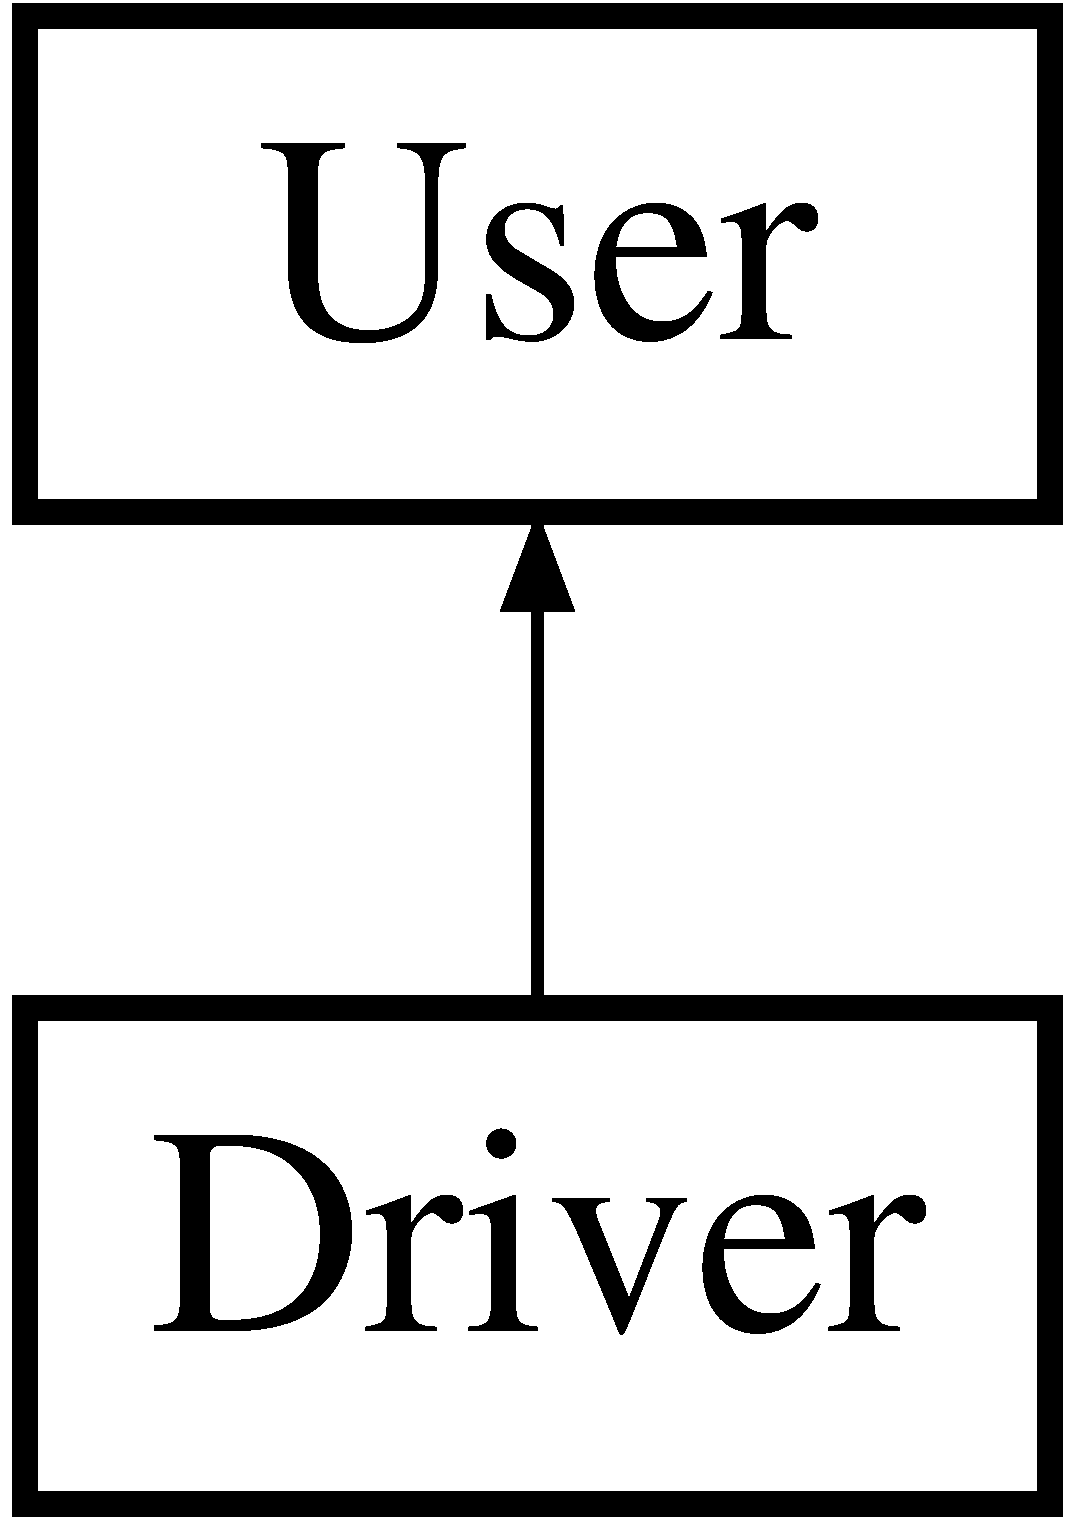
\includegraphics[height=2.000000cm]{class_driver}
\end{center}
\end{figure}
\subsection*{Public Member Functions}
\begin{DoxyCompactItemize}
\item 
\hyperlink{group___user_ga781d40c6af9f399284149602ead32171}{Driver} (int ID, string name, float balance, string username, string password, int nt, string ad, \hyperlink{class_date}{Date} lastA)
\begin{DoxyCompactList}\small\item\em \hyperlink{class_driver}{Driver} constructor from individual parameters. \end{DoxyCompactList}\item 
float \hyperlink{group___user_ga3e6ec3270b94d43b3865b326e5bcd381}{payment} ()
\begin{DoxyCompactList}\small\item\em Retrieves object\textquotesingle{}s payment based on monthly trips \#. \end{DoxyCompactList}\item 
bool \hyperlink{group___user_gaf8b79bce2879830b12e6f3ec954192a2}{car} () const
\begin{DoxyCompactList}\small\item\em C\+Hecks if object is a driver. \end{DoxyCompactList}\end{DoxyCompactItemize}
\subsection*{Additional Inherited Members}


The documentation for this class was generated from the following files\+:\begin{DoxyCompactItemize}
\item 
E\+:/feup-\/aeda/\+A\+E\+D\+A1617\+Parte2\+\_\+2\+M\+I\+E\+I\+C1\+\_\+\+E/\+Código/\+Trabalho A\+E\+D\+A/User.\+h\item 
E\+:/feup-\/aeda/\+A\+E\+D\+A1617\+Parte2\+\_\+2\+M\+I\+E\+I\+C1\+\_\+\+E/\+Código/\+Trabalho A\+E\+D\+A/User.\+cpp\end{DoxyCompactItemize}

\hypertarget{class_error}{}\section{Error Class Reference}
\label{class_error}\index{Error@{Error}}
\subsection*{Public Member Functions}
\begin{DoxyCompactItemize}
\item 
\mbox{\Hypertarget{class_error_a50648efaa6adc6a84b7c90c99d47a99c}\label{class_error_a50648efaa6adc6a84b7c90c99d47a99c}} 
{\bfseries Error} (int n)
\end{DoxyCompactItemize}
\subsection*{Public Attributes}
\begin{DoxyCompactItemize}
\item 
\mbox{\Hypertarget{class_error_a009048d633be19ff0ec45acd04475695}\label{class_error_a009048d633be19ff0ec45acd04475695}} 
int {\bfseries m}
\end{DoxyCompactItemize}


The documentation for this class was generated from the following file\+:\begin{DoxyCompactItemize}
\item 
E\+:/feup-\/aeda/\+A\+E\+D\+A1617\+Parte2\+\_\+2\+M\+I\+E\+I\+C1\+\_\+\+E/\+Código/\+Trabalho A\+E\+D\+A/Agency.\+cpp\end{DoxyCompactItemize}

\hypertarget{class_hour}{}\section{Hour Class Reference}
\label{class_hour}\index{Hour@{Hour}}
\subsection*{Public Member Functions}
\begin{DoxyCompactItemize}
\item 
\hyperlink{group___hour_ga57b604e71195671d96ef6b8e7b819a71}{Hour} ()
\begin{DoxyCompactList}\small\item\em \hyperlink{class_hour}{Hour} default constructor. \end{DoxyCompactList}\item 
\hyperlink{group___hour_ga77024d0dee349bc56162428af7c60f8c}{Hour} (string hour)
\begin{DoxyCompactList}\small\item\em \hyperlink{class_hour}{Hour} constructor from string. \end{DoxyCompactList}\item 
\hyperlink{group___hour_gaedd062589c21da403d9490a9706c3005}{Hour} (int hour, int minutes)
\begin{DoxyCompactList}\small\item\em \hyperlink{class_hour}{Hour} constructor from individual integers. \end{DoxyCompactList}\item 
bool \hyperlink{group___hour_ga1643bbcd2a1b14cd49f45955c62e8ce1}{valid\+Hour} ()
\begin{DoxyCompactList}\small\item\em Checks if the object of class \hyperlink{class_hour}{Hour} is valid by evaluating it\textquotesingle{}s private data on logical validity in the real-\/world. \end{DoxyCompactList}\item 
void \hyperlink{group___hour_ga641c0cf6dd5156a61d5f7f829891b42f}{set\+Current} ()
\begin{DoxyCompactList}\small\item\em Sets object to be the current system\textquotesingle{}s hour. \end{DoxyCompactList}\end{DoxyCompactItemize}
\begin{Indent}\textbf{ Basic Class Functions}\par
\begin{DoxyCompactItemize}
\item 
int \hyperlink{group___hour_ga44859e9acda4578bc3cfcad5d2f25585}{get\+Hour} () const
\begin{DoxyCompactList}\small\item\em Retrieves object\textquotesingle{}s hour. \end{DoxyCompactList}\item 
int \hyperlink{group___hour_gaccf1de7229b52b59d2119e9802fa3eee}{get\+Minutes} () const
\begin{DoxyCompactList}\small\item\em Retrieves object\textquotesingle{}s minutes. \end{DoxyCompactList}\item 
void \hyperlink{group___hour_ga62d4e3da6eeefecab589a63160493835}{set\+Hour} (int hour)
\begin{DoxyCompactList}\small\item\em Sets object\textquotesingle{}s hour. \end{DoxyCompactList}\item 
void \hyperlink{group___hour_gab3606a7c5dd8679a44e79536a491923e}{set\+Minutes} (int mimnutes)
\begin{DoxyCompactList}\small\item\em Sets object\textquotesingle{}s minutes. \end{DoxyCompactList}\end{DoxyCompactItemize}
\end{Indent}
\subsection*{Private Attributes}
\begin{Indent}\textbf{ Hour data-\/members}\par
\begin{DoxyCompactItemize}
\item 
int {\bfseries hour}
\item 
int {\bfseries minutes}
\end{DoxyCompactItemize}
\end{Indent}
\subsection*{Hour Operators Functions}
\begin{DoxyCompactItemize}
\item 
bool \hyperlink{group___hour_ga998bef44d3ea319e70f9d88ad053563b}{operator$<$} (const \hyperlink{class_hour}{Hour} \&h2) const
\begin{DoxyCompactList}\small\item\em Compares two objects of the class to check if one hour if previous to the other. \end{DoxyCompactList}\item 
ostream \& \hyperlink{group___hour_gac58157e808c8f449b403949cbd1b2737}{operator$<$$<$} (ostream \&out, \hyperlink{class_hour}{Hour} \&hour)
\begin{DoxyCompactList}\small\item\em Writes to ostream the information of a object of class \hyperlink{class_hour}{Hour}. \end{DoxyCompactList}\end{DoxyCompactItemize}


The documentation for this class was generated from the following files\+:\begin{DoxyCompactItemize}
\item 
E\+:/feup-\/aeda/\+A\+E\+D\+A1617\+Parte2\+\_\+2\+M\+I\+E\+I\+C1\+\_\+\+E/\+Código/\+Trabalho A\+E\+D\+A/Hour.\+h\item 
E\+:/feup-\/aeda/\+A\+E\+D\+A1617\+Parte2\+\_\+2\+M\+I\+E\+I\+C1\+\_\+\+E/\+Código/\+Trabalho A\+E\+D\+A/Hour.\+cpp\end{DoxyCompactItemize}

\hypertarget{structinactive_ptr}{}\section{inactive\+Ptr Struct Reference}
\label{structinactive_ptr}\index{inactive\+Ptr@{inactive\+Ptr}}


{\ttfamily \#include $<$Agency.\+h$>$}

\subsection*{Public Member Functions}
\begin{DoxyCompactItemize}
\item 
int {\bfseries operator()} (const \hyperlink{structuser_ptr}{user\+Ptr} \&us1) const
\item 
bool {\bfseries operator()} (const \hyperlink{structuser_ptr}{user\+Ptr} \&us1, const \hyperlink{structuser_ptr}{user\+Ptr} \&us2) const
\end{DoxyCompactItemize}


\subsection{Detailed Description}
Struct that keeps the functions in use for the hash table 

The documentation for this struct was generated from the following file\+:\begin{DoxyCompactItemize}
\item 
E\+:/feup-\/aeda/\+A\+E\+D\+A1617\+Parte2\+\_\+2\+M\+I\+E\+I\+C1\+\_\+\+E/\+Código/\+Trabalho A\+E\+D\+A/Agency.\+h\end{DoxyCompactItemize}

\hypertarget{class_invalid_date}{}\section{Invalid\+Date Class Reference}
\label{class_invalid_date}\index{Invalid\+Date@{Invalid\+Date}}
\subsection*{Public Member Functions}
\begin{DoxyCompactItemize}
\item 
\mbox{\Hypertarget{class_invalid_date_a9cccc591c3a07535f26d1ec06b4087fd}\label{class_invalid_date_a9cccc591c3a07535f26d1ec06b4087fd}} 
{\bfseries Invalid\+Date} (\hyperlink{class_date}{Date} d)
\end{DoxyCompactItemize}
\subsection*{Public Attributes}
\begin{DoxyCompactItemize}
\item 
\mbox{\Hypertarget{class_invalid_date_a22b43ab189cf85971b69f8a7e363edbe}\label{class_invalid_date_a22b43ab189cf85971b69f8a7e363edbe}} 
\hyperlink{class_date}{Date} {\bfseries date}
\end{DoxyCompactItemize}


The documentation for this class was generated from the following file\+:\begin{DoxyCompactItemize}
\item 
E\+:/feup-\/aeda/\+A\+E\+D\+A1617\+Parte2\+\_\+2\+M\+I\+E\+I\+C1\+\_\+\+E/\+Código/\+Trabalho A\+E\+D\+A/Agency.\+cpp\end{DoxyCompactItemize}

\hypertarget{class_invalid_hour}{}\section{Invalid\+Hour Class Reference}
\label{class_invalid_hour}\index{Invalid\+Hour@{Invalid\+Hour}}
\subsection*{Public Member Functions}
\begin{DoxyCompactItemize}
\item 
\mbox{\Hypertarget{class_invalid_hour_aa69c39a6d6e2012fc1e908c81141f3bb}\label{class_invalid_hour_aa69c39a6d6e2012fc1e908c81141f3bb}} 
{\bfseries Invalid\+Hour} (int h, int m)
\end{DoxyCompactItemize}
\subsection*{Public Attributes}
\begin{DoxyCompactItemize}
\item 
\mbox{\Hypertarget{class_invalid_hour_ab0fd96c9274552f16757b1ef9c802b1a}\label{class_invalid_hour_ab0fd96c9274552f16757b1ef9c802b1a}} 
int {\bfseries hour}
\item 
\mbox{\Hypertarget{class_invalid_hour_a4474b11b0d644762b773694d622b0ef1}\label{class_invalid_hour_a4474b11b0d644762b773694d622b0ef1}} 
int {\bfseries minutes}
\end{DoxyCompactItemize}


The documentation for this class was generated from the following file\+:\begin{DoxyCompactItemize}
\item 
E\+:/feup-\/aeda/\+A\+E\+D\+A1617\+Parte2\+\_\+2\+M\+I\+E\+I\+C1\+\_\+\+E/\+Código/\+Trabalho A\+E\+D\+A/Agency.\+cpp\end{DoxyCompactItemize}

\hypertarget{class_nonexistent_car}{}\section{Nonexistent\+Car Class Reference}
\label{class_nonexistent_car}\index{Nonexistent\+Car@{Nonexistent\+Car}}


The documentation for this class was generated from the following file\+:\begin{DoxyCompactItemize}
\item 
E\+:/feup-\/aeda/\+A\+E\+D\+A1617\+Parte2\+\_\+2\+M\+I\+E\+I\+C1\+\_\+\+E/\+Código/\+Trabalho A\+E\+D\+A/Agency.\+cpp\end{DoxyCompactItemize}

\hypertarget{class_nonexistent_stop}{}\section{Nonexistent\+Stop Class Reference}
\label{class_nonexistent_stop}\index{Nonexistent\+Stop@{Nonexistent\+Stop}}
\subsection*{Public Member Functions}
\begin{DoxyCompactItemize}
\item 
\mbox{\Hypertarget{class_nonexistent_stop_a68e23a1955374c63909d5c8abd80585a}\label{class_nonexistent_stop_a68e23a1955374c63909d5c8abd80585a}} 
{\bfseries Nonexistent\+Stop} (string name)
\end{DoxyCompactItemize}
\subsection*{Public Attributes}
\begin{DoxyCompactItemize}
\item 
\mbox{\Hypertarget{class_nonexistent_stop_a3083f3480d02646b96e3291fedaf9615}\label{class_nonexistent_stop_a3083f3480d02646b96e3291fedaf9615}} 
string {\bfseries stop}
\end{DoxyCompactItemize}


The documentation for this class was generated from the following file\+:\begin{DoxyCompactItemize}
\item 
E\+:/feup-\/aeda/\+A\+E\+D\+A1617\+Parte2\+\_\+2\+M\+I\+E\+I\+C1\+\_\+\+E/\+Código/\+Trabalho A\+E\+D\+A/Agency.\+cpp\end{DoxyCompactItemize}

\hypertarget{class_passed_date}{}\section{Passed\+Date Class Reference}
\label{class_passed_date}\index{Passed\+Date@{Passed\+Date}}
\subsection*{Public Member Functions}
\begin{DoxyCompactItemize}
\item 
\mbox{\Hypertarget{class_passed_date_aa2d8f7f8b8bdf1b1ba51d64b39ced632}\label{class_passed_date_aa2d8f7f8b8bdf1b1ba51d64b39ced632}} 
{\bfseries Passed\+Date} (int d, int m, int y)
\end{DoxyCompactItemize}
\subsection*{Public Attributes}
\begin{DoxyCompactItemize}
\item 
\mbox{\Hypertarget{class_passed_date_a9d8af874932e7d9b3905740997bcb03d}\label{class_passed_date_a9d8af874932e7d9b3905740997bcb03d}} 
int {\bfseries day}
\item 
\mbox{\Hypertarget{class_passed_date_a619002f7f79228fbf4bc26f28cd055a2}\label{class_passed_date_a619002f7f79228fbf4bc26f28cd055a2}} 
int {\bfseries month}
\item 
\mbox{\Hypertarget{class_passed_date_a0ca79bcf75538befd1543ccdeb8be9a5}\label{class_passed_date_a0ca79bcf75538befd1543ccdeb8be9a5}} 
int {\bfseries year}
\end{DoxyCompactItemize}


The documentation for this class was generated from the following file\+:\begin{DoxyCompactItemize}
\item 
E\+:/feup-\/aeda/\+A\+E\+D\+A1617\+Parte2\+\_\+2\+M\+I\+E\+I\+C1\+\_\+\+E/\+Código/\+Trabalho A\+E\+D\+A/Agency.\+cpp\end{DoxyCompactItemize}

\hypertarget{class_passed_hour}{}\section{Passed\+Hour Class Reference}
\label{class_passed_hour}\index{Passed\+Hour@{Passed\+Hour}}
\subsection*{Public Member Functions}
\begin{DoxyCompactItemize}
\item 
\mbox{\Hypertarget{class_passed_hour_aebd27de85dd95fde6655fd2037356f84}\label{class_passed_hour_aebd27de85dd95fde6655fd2037356f84}} 
{\bfseries Passed\+Hour} (int h, int m)
\end{DoxyCompactItemize}
\subsection*{Public Attributes}
\begin{DoxyCompactItemize}
\item 
\mbox{\Hypertarget{class_passed_hour_a07abcad6d6d0d5d3fa5a5fe7981d52b7}\label{class_passed_hour_a07abcad6d6d0d5d3fa5a5fe7981d52b7}} 
int {\bfseries hour}
\item 
\mbox{\Hypertarget{class_passed_hour_ab371a82e5e3cc1219630cc6c32cb0daa}\label{class_passed_hour_ab371a82e5e3cc1219630cc6c32cb0daa}} 
int {\bfseries minutes}
\end{DoxyCompactItemize}


The documentation for this class was generated from the following file\+:\begin{DoxyCompactItemize}
\item 
E\+:/feup-\/aeda/\+A\+E\+D\+A1617\+Parte2\+\_\+2\+M\+I\+E\+I\+C1\+\_\+\+E/\+Código/\+Trabalho A\+E\+D\+A/Agency.\+cpp\end{DoxyCompactItemize}

\hypertarget{class_passenger}{}\section{Passenger Class Reference}
\label{class_passenger}\index{Passenger@{Passenger}}
Inheritance diagram for Passenger\+:\begin{figure}[H]
\begin{center}
\leavevmode
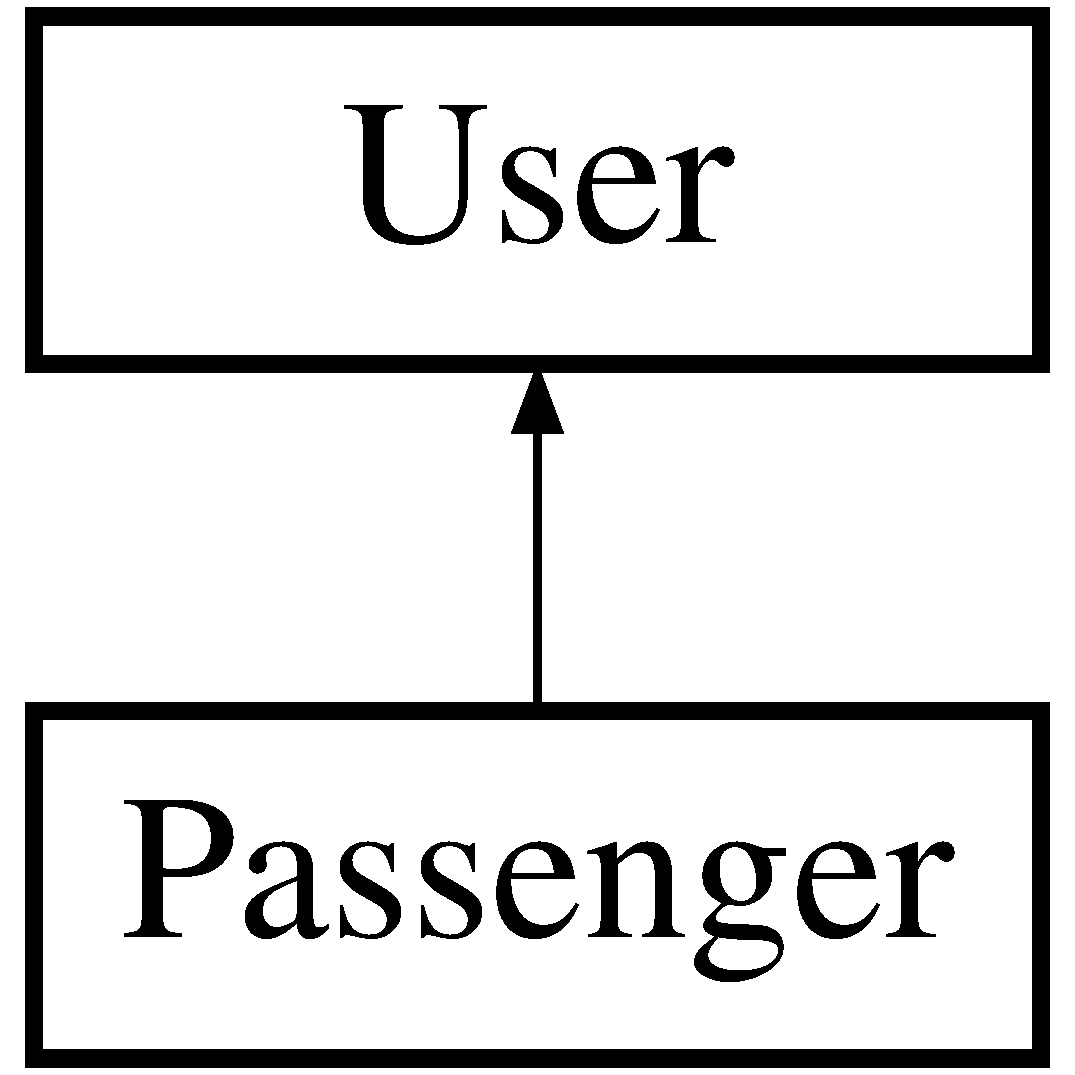
\includegraphics[height=2.000000cm]{class_passenger}
\end{center}
\end{figure}
\subsection*{Public Member Functions}
\begin{DoxyCompactItemize}
\item 
\hyperlink{group___user_ga00628e580d270e68278cc76994c841b1}{Passenger} (string name)
\begin{DoxyCompactList}\small\item\em \hyperlink{class_user}{User} constructor from individual parameter. \end{DoxyCompactList}\item 
\hyperlink{group___user_ga0c1aecc465a9e8887f2b9bd3e784438a}{Passenger} (int ID, string name, float balance, string username, string password, int nt, string ad, \hyperlink{class_date}{Date} lastA)
\begin{DoxyCompactList}\small\item\em \hyperlink{class_passenger}{Passenger} constructor from individual parameters. \end{DoxyCompactList}\item 
float \hyperlink{group___user_ga9535b6486d1f33f055d6c7385780ec68}{payment} ()
\begin{DoxyCompactList}\small\item\em Retrieves object\textquotesingle{}s payment based on monthly trips \#. \end{DoxyCompactList}\item 
bool \hyperlink{group___user_gaeb69b29d53079577e41f070da1f442dd}{car} () const
\begin{DoxyCompactList}\small\item\em Checks if object is a driver. \end{DoxyCompactList}\end{DoxyCompactItemize}
\subsection*{Additional Inherited Members}


The documentation for this class was generated from the following files\+:\begin{DoxyCompactItemize}
\item 
E\+:/feup-\/aeda/\+A\+E\+D\+A1617\+Parte2\+\_\+2\+M\+I\+E\+I\+C1\+\_\+\+E/\+Código/\+Trabalho A\+E\+D\+A/User.\+h\item 
E\+:/feup-\/aeda/\+A\+E\+D\+A1617\+Parte2\+\_\+2\+M\+I\+E\+I\+C1\+\_\+\+E/\+Código/\+Trabalho A\+E\+D\+A/User.\+cpp\end{DoxyCompactItemize}

\hypertarget{class_repeated_stop}{}\section{Repeated\+Stop Class Reference}
\label{class_repeated_stop}\index{Repeated\+Stop@{Repeated\+Stop}}
\subsection*{Public Member Functions}
\begin{DoxyCompactItemize}
\item 
\mbox{\Hypertarget{class_repeated_stop_a5d20d59ad7402d38d9a3605fd28180b8}\label{class_repeated_stop_a5d20d59ad7402d38d9a3605fd28180b8}} 
{\bfseries Repeated\+Stop} (string name)
\end{DoxyCompactItemize}
\subsection*{Public Attributes}
\begin{DoxyCompactItemize}
\item 
\mbox{\Hypertarget{class_repeated_stop_a7c050f1a63c4344eee67fca69be0f44b}\label{class_repeated_stop_a7c050f1a63c4344eee67fca69be0f44b}} 
string {\bfseries stop}
\end{DoxyCompactItemize}


The documentation for this class was generated from the following file\+:\begin{DoxyCompactItemize}
\item 
E\+:/feup-\/aeda/\+A\+E\+D\+A1617\+Parte2\+\_\+2\+M\+I\+E\+I\+C1\+\_\+\+E/\+Código/\+Trabalho A\+E\+D\+A/Agency.\+cpp\end{DoxyCompactItemize}

\hypertarget{structstop}{}\section{stop Struct Reference}
\label{structstop}\index{stop@{stop}}


{\ttfamily \#include $<$Agency.\+h$>$}

\subsection*{Public Attributes}
\begin{DoxyCompactItemize}
\item 
string {\bfseries code}
\item 
string {\bfseries name}
\end{DoxyCompactItemize}


\subsection{Detailed Description}
Struct that keeps info regarding the name and code of a stop 

The documentation for this struct was generated from the following file\+:\begin{DoxyCompactItemize}
\item 
E\+:/feup-\/aeda/\+A\+E\+D\+A1617\+Parte2\+\_\+2\+M\+I\+E\+I\+C1\+\_\+\+E/\+Código/\+Trabalho A\+E\+D\+A/Agency.\+h\end{DoxyCompactItemize}

\hypertarget{class_stop}{}\section{Stop Class Reference}
\label{class_stop}\index{Stop@{Stop}}
\subsection*{Public Member Functions}
\begin{DoxyCompactItemize}
\item 
\hyperlink{group___stop_gab8870f949c69cda03c4055524ed13c31}{Stop} ()
\begin{DoxyCompactList}\small\item\em \hyperlink{class_stop}{Stop} default constructor. \end{DoxyCompactList}\item 
\hyperlink{group___stop_gaa89c250884ae1407ac8647a8a3a58995}{Stop} (string \hyperlink{group___stop_ga5a0dddd108225fd437be86eed7b3a3ef}{code}, int seats)
\begin{DoxyCompactList}\small\item\em \hyperlink{class_date}{Date} constructor from individual parameters. \end{DoxyCompactList}\item 
\hyperlink{group___stop_ga843a7424de0129e7f6f066d2f8f1d1bc}{Stop} (string \hyperlink{group___stop_ga5a0dddd108225fd437be86eed7b3a3ef}{code}, int seats, vector$<$ int $>$ vpass)
\begin{DoxyCompactList}\small\item\em \hyperlink{class_date}{Date} constructor from individual parameters. \end{DoxyCompactList}\item 
\hyperlink{group___stop_ga24e85edfa98a7a0212136679b6fad6d2}{$\sim$\+Stop} ()
\begin{DoxyCompactList}\small\item\em \hyperlink{class_stop}{Stop} default destructor. \end{DoxyCompactList}\end{DoxyCompactItemize}
\begin{Indent}\textbf{ Basic Class Functions}\par
\begin{DoxyCompactItemize}
\item 
string \hyperlink{group___stop_ga4c0a7bb72ca7a054a394d13fc8cd9bde}{get\+Code} () const
\begin{DoxyCompactList}\small\item\em Retrieves the object\textquotesingle{}s code. \end{DoxyCompactList}\item 
int \hyperlink{group___stop_ga41d42147d1210ce72f15e31a8414e0ad}{get\+Available\+Seats} () const
\begin{DoxyCompactList}\small\item\em Retrieves the object\textquotesingle{}s number of available seats. \end{DoxyCompactList}\item 
vector$<$ int $>$ \hyperlink{group___stop_gabd197ec53b1215bed050d879d463e987}{get\+Passengers} () const
\begin{DoxyCompactList}\small\item\em Retrieves the object\textquotesingle{}s vector of passengers I\+Ds. \end{DoxyCompactList}\item 
void \hyperlink{group___stop_ga491669933a1b091fa543591e9fd992aa}{dec\+Available\+Seats} ()
\begin{DoxyCompactList}\small\item\em Decrements the object\textquotesingle{}s number of available seats by 1. \end{DoxyCompactList}\item 
void \hyperlink{group___stop_gac636e3c0c1e2794575bd3db14b5ee363}{add\+Passenger} (int id)
\begin{DoxyCompactList}\small\item\em Adds the ID of a passenger to the object\textquotesingle{}s vector of I\+Ds. \end{DoxyCompactList}\end{DoxyCompactItemize}
\end{Indent}
\subsection*{Private Attributes}
\begin{Indent}\textbf{ Stop data-\/members}\par
\begin{DoxyCompactItemize}
\item 
string \hyperlink{group___stop_ga5a0dddd108225fd437be86eed7b3a3ef}{code}
\begin{DoxyCompactList}\small\item\em string of 3 letters that represents the code of a stop \end{DoxyCompactList}\item 
int \hyperlink{group___stop_ga459aba5bcfa17889d2f292f3f45528bc}{available\+Seats}
\begin{DoxyCompactList}\small\item\em Number of available seats at a stop. \end{DoxyCompactList}\item 
vector$<$ int $>$ \hyperlink{group___stop_ga2886c8f28932f3884ba3e4f741e7ec91}{passengers}
\begin{DoxyCompactList}\small\item\em vector containing the I\+Ds of the passengers present at that stop \end{DoxyCompactList}\end{DoxyCompactItemize}
\end{Indent}


The documentation for this class was generated from the following files\+:\begin{DoxyCompactItemize}
\item 
E\+:/feup-\/aeda/\+A\+E\+D\+A1617\+Parte2\+\_\+2\+M\+I\+E\+I\+C1\+\_\+\+E/\+Código/\+Trabalho A\+E\+D\+A/Stop.\+h\item 
E\+:/feup-\/aeda/\+A\+E\+D\+A1617\+Parte2\+\_\+2\+M\+I\+E\+I\+C1\+\_\+\+E/\+Código/\+Trabalho A\+E\+D\+A/Stop.\+cpp\end{DoxyCompactItemize}

\hypertarget{class_too_long}{}\section{Too\+Long Class Reference}
\label{class_too_long}\index{Too\+Long@{Too\+Long}}
\subsection*{Public Member Functions}
\begin{DoxyCompactItemize}
\item 
\mbox{\Hypertarget{class_too_long_a6221d3bc68906de82093e730a7e02358}\label{class_too_long_a6221d3bc68906de82093e730a7e02358}} 
{\bfseries Too\+Long} (int d, int m, int y)
\end{DoxyCompactItemize}
\subsection*{Public Attributes}
\begin{DoxyCompactItemize}
\item 
\mbox{\Hypertarget{class_too_long_a95367d0bbb25178e4df2b951e091318a}\label{class_too_long_a95367d0bbb25178e4df2b951e091318a}} 
int {\bfseries day}
\item 
\mbox{\Hypertarget{class_too_long_a51bb8be6bc22cf1dd32f814734693889}\label{class_too_long_a51bb8be6bc22cf1dd32f814734693889}} 
int {\bfseries month}
\item 
\mbox{\Hypertarget{class_too_long_af665a5e1f89b62152ab6edfa92a2f109}\label{class_too_long_af665a5e1f89b62152ab6edfa92a2f109}} 
int {\bfseries year}
\end{DoxyCompactItemize}


The documentation for this class was generated from the following file\+:\begin{DoxyCompactItemize}
\item 
E\+:/feup-\/aeda/\+A\+E\+D\+A1617\+Parte2\+\_\+2\+M\+I\+E\+I\+C1\+\_\+\+E/\+Código/\+Trabalho A\+E\+D\+A/Agency.\+cpp\end{DoxyCompactItemize}

\hypertarget{class_transaction}{}\section{Transaction Class Reference}
\label{class_transaction}\index{Transaction@{Transaction}}
\subsection*{Public Member Functions}
\begin{DoxyCompactItemize}
\item 
\hyperlink{group___transaction_gab47005b855d38bc324bb79fd023baa13}{Transaction} ()
\begin{DoxyCompactList}\small\item\em \hyperlink{class_transaction}{Transaction} default constructor. \end{DoxyCompactList}\item 
\hyperlink{group___transaction_ga6bba02c02aace16e90745fecd2e4697d}{Transaction} (int id, \hyperlink{class_date}{Date} date, float value)
\begin{DoxyCompactList}\small\item\em \hyperlink{class_transaction}{Transaction} constructor from individual parameters. \end{DoxyCompactList}\item 
void \hyperlink{group___transaction_ga56b1bd622e55266bf795fb01e04e8a21}{save} (ofstream \&out) const
\begin{DoxyCompactList}\small\item\em Writes object\textquotesingle{}s information into file. \end{DoxyCompactList}\end{DoxyCompactItemize}
\begin{Indent}\textbf{ Basic Class Functions}\par
\begin{DoxyCompactItemize}
\item 
int \hyperlink{group___transaction_ga73ff525f9baae732b1256533736e5052}{Get\+Id} () const
\begin{DoxyCompactList}\small\item\em Retrieves object\textquotesingle{}s ID. \end{DoxyCompactList}\item 
\hyperlink{class_date}{Date} \hyperlink{group___transaction_ga05b17fe71d38937648b77f964df4de5d}{Get\+Date} () const
\begin{DoxyCompactList}\small\item\em Retrieves object\textquotesingle{}s \hyperlink{class_date}{Date}. \end{DoxyCompactList}\item 
float \hyperlink{group___transaction_ga3dca9a51e64e6fcb07f501eb2724676d}{Get\+Value} () const
\begin{DoxyCompactList}\small\item\em Retrieves object\textquotesingle{}s value. \end{DoxyCompactList}\end{DoxyCompactItemize}
\end{Indent}
\subsection*{Private Attributes}
\begin{Indent}\textbf{ Transaction data-\/members}\par
\begin{DoxyCompactItemize}
\item 
int {\bfseries id}
\item 
\hyperlink{class_date}{Date} {\bfseries date}
\item 
float {\bfseries value}
\end{DoxyCompactItemize}
\end{Indent}
\subsection*{Friends}
\begin{Indent}\textbf{ Transaction Operators Functions}\par
\begin{DoxyCompactItemize}
\item 
ostream \& \hyperlink{group___transaction_ga75af23fbc3b593013d411cf50c5a3a7a}{operator$<$$<$} (ostream \&out, const \hyperlink{class_transaction}{Transaction} \&t)
\begin{DoxyCompactList}\small\item\em Writes to ostream the information of a object of class \hyperlink{class_transaction}{Transaction}. \end{DoxyCompactList}\end{DoxyCompactItemize}
\end{Indent}


The documentation for this class was generated from the following files\+:\begin{DoxyCompactItemize}
\item 
E\+:/feup-\/aeda/\+A\+E\+D\+A1617\+Parte2\+\_\+2\+M\+I\+E\+I\+C1\+\_\+\+E/\+Código/\+Trabalho A\+E\+D\+A/Transactions.\+h\item 
E\+:/feup-\/aeda/\+A\+E\+D\+A1617\+Parte2\+\_\+2\+M\+I\+E\+I\+C1\+\_\+\+E/\+Código/\+Trabalho A\+E\+D\+A/Transactions.\+cpp\end{DoxyCompactItemize}

\hypertarget{class_trip}{}\section{Trip Class Reference}
\label{class_trip}\index{Trip@{Trip}}
\subsection*{Public Member Functions}
\begin{DoxyCompactItemize}
\item 
\hyperlink{group___trip_gaa67b77d0d2de622ed5eb9e9cad34db8f}{Trip} ()
\begin{DoxyCompactList}\small\item\em \hyperlink{class_trip}{Trip} default constructor. \end{DoxyCompactList}\item 
\hyperlink{group___trip_gaadf8ba70a9d5aa210149b5162e402512}{Trip} (int ID, int driver, vector$<$ \hyperlink{class_stop}{Stop} $>$ stops, \hyperlink{class_date}{Date} date, \hyperlink{class_hour}{Hour} start, \hyperlink{class_hour}{Hour} end)
\begin{DoxyCompactList}\small\item\em \hyperlink{class_trip}{Trip} constructor from individual parameters. \end{DoxyCompactList}\item 
\hyperlink{group___trip_ga2376daed3b03469163782ef0d0533d52}{$\sim$\+Trip} ()
\begin{DoxyCompactList}\small\item\em \hyperlink{class_trip}{Trip} destructor. \end{DoxyCompactList}\item 
void \hyperlink{group___trip_ga6ae6134652b644fa63bf267b956f1e75}{save} (ofstream \&out) const
\begin{DoxyCompactList}\small\item\em Writes object\textquotesingle{}s information into file. \end{DoxyCompactList}\item 
void \hyperlink{group___trip_gafcf569c0a9d6e5a47134f7e9dd62334a}{save\+AT} (ofstream \&out) const
\begin{DoxyCompactList}\small\item\em Writes object\textquotesingle{}s information into file (only for active trips, to remain in the program for next use) \end{DoxyCompactList}\end{DoxyCompactItemize}
\begin{Indent}\textbf{ Basic Class Functions}\par
\begin{DoxyCompactItemize}
\item 
int \hyperlink{group___trip_gabc996cddbc65b41987dd8d4d9776c729}{get\+Driver} () const
\begin{DoxyCompactList}\small\item\em Retrieves object\textquotesingle{}s driver. \end{DoxyCompactList}\item 
int \hyperlink{group___trip_ga61fea247b075bfac3f6115da4bd56ef5}{get\+ID} () const
\begin{DoxyCompactList}\small\item\em Retrieves object\textquotesingle{}s ID. \end{DoxyCompactList}\item 
vector$<$ \hyperlink{class_stop}{Stop} $>$ \hyperlink{group___trip_gae081fb958af544c9cad9002d5696fb33}{get\+Stops} () const
\begin{DoxyCompactList}\small\item\em Retrieves object\textquotesingle{}s vector of stops. \end{DoxyCompactList}\item 
\hyperlink{class_date}{Date} \hyperlink{group___trip_ga322346fb52d53fb0a94819059916d0fe}{get\+Date} () const
\begin{DoxyCompactList}\small\item\em Retrieves object\textquotesingle{}s \hyperlink{class_date}{Date}. \end{DoxyCompactList}\item 
\hyperlink{class_hour}{Hour} \hyperlink{group___trip_ga447efbf91bd4842daadac85d2bac4b9e}{get\+Start} () const
\begin{DoxyCompactList}\small\item\em Retrieves object\textquotesingle{}s starting hour. \end{DoxyCompactList}\item 
\hyperlink{class_hour}{Hour} \hyperlink{group___trip_ga6ed6b87b4206efe21fe2c6744c73061b}{get\+End} () const
\begin{DoxyCompactList}\small\item\em Retrieves object\textquotesingle{}s estimated finishing hour. \end{DoxyCompactList}\item 
string \hyperlink{group___trip_gaf63e96a9b31ad6def658944bc6a9f327}{get\+Origin} () const
\begin{DoxyCompactList}\small\item\em Retrieves object\textquotesingle{}s origin stop. \end{DoxyCompactList}\item 
string \hyperlink{group___trip_ga576ad0d4c7a723aa4b2d12ebdd4eec99}{get\+Destination} () const
\begin{DoxyCompactList}\small\item\em Retrieves object\textquotesingle{}s destination stop. \end{DoxyCompactList}\item 
void \hyperlink{group___trip_ga2c5c0c0315b210154ba190a5470ec110}{set\+Driver} (int id)
\begin{DoxyCompactList}\small\item\em Sets object\textquotesingle{}s driver id. \end{DoxyCompactList}\item 
void \hyperlink{group___trip_ga26abc8edc0cb1f5c2eb1b6e292152701}{set\+Date} (\hyperlink{class_date}{Date} d)
\begin{DoxyCompactList}\small\item\em Sets object\textquotesingle{}s \hyperlink{class_date}{Date}. \end{DoxyCompactList}\item 
void \hyperlink{group___trip_gaa294f1f8844c2b47676e0e985d81b2a0}{set\+Stops} (int pos, int user\+ID)
\begin{DoxyCompactList}\small\item\em Changes object\textquotesingle{}s stops ir order to add a passenger. \end{DoxyCompactList}\end{DoxyCompactItemize}
\end{Indent}
\subsection*{Private Attributes}
\begin{Indent}\textbf{ Trip data-\/members}\par
\begin{DoxyCompactItemize}
\item 
int {\bfseries ID}
\item 
int {\bfseries driver}
\item 
vector$<$ \hyperlink{class_stop}{Stop} $>$ {\bfseries stops}
\item 
\hyperlink{class_date}{Date} {\bfseries date}
\item 
\hyperlink{class_hour}{Hour} {\bfseries start\+Time}
\item 
\hyperlink{class_hour}{Hour} {\bfseries end\+Time}
\item 
priority\+\_\+queue$<$ \hyperlink{class_candidate_trip}{Candidate\+Trip} $>$ {\bfseries candidate\+Queue}
\end{DoxyCompactItemize}
\end{Indent}
\subsection*{Trip Operators Functions}
\begin{DoxyCompactItemize}
\item 
bool \hyperlink{group___trip_ga1462791c70b237e595244b16e086850f}{operator==} (const \hyperlink{class_trip}{Trip} t) const
\begin{DoxyCompactList}\small\item\em Basi operator that verifies if two diferent objects of the class \hyperlink{class_trip}{Trip} have equal data members. \end{DoxyCompactList}\item 
priority\+\_\+queue$<$ \hyperlink{class_candidate_trip}{Candidate\+Trip} $>$ \hyperlink{group___trip_ga1c016b992e17387a25ec9f7e545a6594}{get\+Candidate\+Queue} () const
\begin{DoxyCompactList}\small\item\em Retrieves object\textquotesingle{}s candidates priority queuu. \end{DoxyCompactList}\item 
bool \hyperlink{group___trip_gaa704cf099858e8de479f6fdd6229008f}{is\+In\+Queue} (int id)
\begin{DoxyCompactList}\small\item\em verifyes if the user is in this trip queue \end{DoxyCompactList}\item 
void \hyperlink{group___trip_ga6879d39109d9b024461c9edb58c8b1dd}{add\+Candidate} (\hyperlink{class_candidate_trip}{Candidate\+Trip} ct)
\begin{DoxyCompactList}\small\item\em adds elements to the priority queue \end{DoxyCompactList}\item 
void \hyperlink{group___trip_ga5c0fbf9c2320dc4799896295788eff9e}{remove\+Candidate} (int id)
\begin{DoxyCompactList}\small\item\em removes user from the queue \end{DoxyCompactList}\item 
ostream \& \hyperlink{group___trip_gaeae00f4e739b064d8261c91d62cde34a}{operator$<$$<$} (ostream \&out, const \hyperlink{class_trip}{Trip} \&t)
\begin{DoxyCompactList}\small\item\em Writes to ostream the information of a object of class \hyperlink{class_trip}{Trip}. \end{DoxyCompactList}\end{DoxyCompactItemize}


The documentation for this class was generated from the following files\+:\begin{DoxyCompactItemize}
\item 
E\+:/feup-\/aeda/\+A\+E\+D\+A1617\+Parte2\+\_\+2\+M\+I\+E\+I\+C1\+\_\+\+E/\+Código/\+Trabalho A\+E\+D\+A/Trip.\+h\item 
E\+:/feup-\/aeda/\+A\+E\+D\+A1617\+Parte2\+\_\+2\+M\+I\+E\+I\+C1\+\_\+\+E/\+Código/\+Trabalho A\+E\+D\+A/Trip.\+cpp\end{DoxyCompactItemize}

\hypertarget{class_user}{}\section{User Class Reference}
\label{class_user}\index{User@{User}}
Inheritance diagram for User\+:\begin{figure}[H]
\begin{center}
\leavevmode
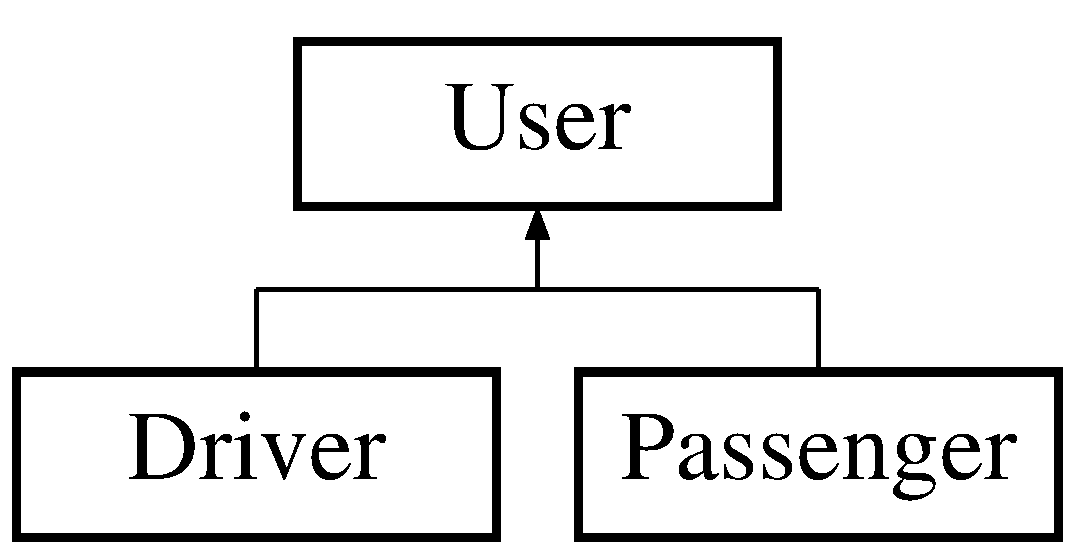
\includegraphics[height=2.000000cm]{class_user}
\end{center}
\end{figure}
\subsection*{Public Member Functions}
\begin{DoxyCompactItemize}
\item 
\hyperlink{group___user_ga4a0137053e591fbb79d9057dd7d2283d}{User} ()
\begin{DoxyCompactList}\small\item\em \hyperlink{class_user}{User} default constructor. \end{DoxyCompactList}\item 
\hyperlink{group___user_gab4d18a829f31eae091669ac36782a396}{User} (string name)
\begin{DoxyCompactList}\small\item\em \hyperlink{class_user}{User} constructor from individual parameter. \end{DoxyCompactList}\item 
\hyperlink{group___user_ga4cad036bd4872821fa6c2585c8778461}{User} (int ID, string name, float balance, string username, string password, int nt, string ad, \hyperlink{class_date}{Date} lastA)
\begin{DoxyCompactList}\small\item\em \hyperlink{class_user}{User} constructor from individual parameters. \end{DoxyCompactList}\item 
\hyperlink{group___user_gac00b72ad64eb4149f7b21b9f5468c2b2}{$\sim$\+User} ()
\begin{DoxyCompactList}\small\item\em \hyperlink{class_user}{User} destructor. \end{DoxyCompactList}\item 
virtual float \hyperlink{group___user_gac8563338d1d8086cd5485ad8c1ed4499}{payment} ()
\begin{DoxyCompactList}\small\item\em Retrieves object\textquotesingle{}s payment based on monthly trips \#. \end{DoxyCompactList}\item 
void \hyperlink{group___user_ga72cde56f7a6c5abcf8a22dcd6fdc8449}{add\+Buddy} (\hyperlink{class_user}{User} $\ast$user)
\begin{DoxyCompactList}\small\item\em Adds \hyperlink{class_user}{User} to vector of Buddies of the object. \end{DoxyCompactList}\item 
void \hyperlink{group___user_gaaaa81787feebf8150cc2553e13edb8f7}{delete\+Buddies} ()
\begin{DoxyCompactList}\small\item\em Resets object\textquotesingle{}s vector of buddies. \end{DoxyCompactList}\item 
vector$<$ \hyperlink{class_user}{User} $\ast$ $>$ \hyperlink{group___user_ga47d6c3dccd2b1c3050fbd0f572bac6f8}{get\+Buddies} () const
\begin{DoxyCompactList}\small\item\em Retrieves object\textquotesingle{}s vector of Buddies. \end{DoxyCompactList}\item 
bool \hyperlink{group___user_gab403e4acde558a3f968aa13b74960da5}{operator==} (const \hyperlink{class_user}{User} $\ast$u) const
\begin{DoxyCompactList}\small\item\em Compares two objects of the class \hyperlink{class_user}{User}. \end{DoxyCompactList}\item 
void {\bfseries set\+Password} (string password)
\item 
void \hyperlink{group___user_ga280617ba3ac500d59e6eb8af09dc3487}{remove\+Buddy} (int ID)
\begin{DoxyCompactList}\small\item\em removes user as buddy of all users \end{DoxyCompactList}\end{DoxyCompactItemize}
\begin{Indent}\textbf{ Basic Class Functions}\par
\begin{DoxyCompactItemize}
\item 
void \hyperlink{group___user_ga0fed77d10cd142ee4112d650ec564e6b}{set\+Username} (string username)
\begin{DoxyCompactList}\small\item\em Sets object\textquotesingle{}s username. \end{DoxyCompactList}\item 
void \hyperlink{group___user_ga95feef2641a3141ef514a0bd52c3aaa2}{set\+ID} (int ID)
\begin{DoxyCompactList}\small\item\em Sets object\textquotesingle{}s ID. \end{DoxyCompactList}\item 
int \hyperlink{group___user_ga986c6f30aeac167bb5d311dd412cf604}{get\+ID} () const
\begin{DoxyCompactList}\small\item\em Retrieves object\textquotesingle{}s ID. \end{DoxyCompactList}\item 
void \hyperlink{group___user_ga5578e73f0915b2ebf38eff4434fc340d}{set\+Last\+Access} (\hyperlink{class_date}{Date} dt)
\begin{DoxyCompactList}\small\item\em Sets object\textquotesingle{}s last access date. \end{DoxyCompactList}\item 
\hyperlink{class_date}{Date} \hyperlink{group___user_ga9399e8ad03d939281357fe2e1d2a0f71}{get\+Last\+Access} () const
\begin{DoxyCompactList}\small\item\em Retrieves object\textquotesingle{}s last access date. \end{DoxyCompactList}\item 
string \hyperlink{group___user_gab9b2b5feb6bdd1582696eb6d44cee384}{get\+Name} () const
\begin{DoxyCompactList}\small\item\em Retrieves object\textquotesingle{}s name. \end{DoxyCompactList}\item 
string \hyperlink{group___user_ga82e034043e04b2d750c654c8b2f2ce78}{get\+Username} () const
\begin{DoxyCompactList}\small\item\em Retrieves object\textquotesingle{}s username. \end{DoxyCompactList}\item 
void \hyperlink{group___user_ga02324144fd363369f11b7aca8f117865}{set\+Adress} (string ad)
\begin{DoxyCompactList}\small\item\em Sets object\textquotesingle{}s address. \end{DoxyCompactList}\item 
string \hyperlink{group___user_gaef1759300db1bca3c84af6af79f00365}{get\+Address} () const
\begin{DoxyCompactList}\small\item\em Retrieves object\textquotesingle{}s address. \end{DoxyCompactList}\item 
string \hyperlink{group___user_ga33429bdd1253091697a9c5c5e1448bee}{get\+Password} () const
\begin{DoxyCompactList}\small\item\em Retrieves object\textquotesingle{}s password. \end{DoxyCompactList}\item 
float \hyperlink{group___user_ga713b20a844b9e70630a50dd5f1357d95}{get\+Balance} () const
\begin{DoxyCompactList}\small\item\em Retrieves object\textquotesingle{}s balance. \end{DoxyCompactList}\item 
int \hyperlink{group___user_gadfbbdc7ea72e051b7b7b8d41c14eb846}{get\+Ntrips} () const
\begin{DoxyCompactList}\small\item\em Retrieves object\textquotesingle{}s \# of trips. \end{DoxyCompactList}\item 
void \hyperlink{group___user_ga738dab753a5a3ba6e1315caaf4765a24}{set\+Ntrips} ()
\begin{DoxyCompactList}\small\item\em Increments object\textquotesingle{}s \# of trips. \end{DoxyCompactList}\item 
void \hyperlink{group___user_ga0b5d245f2e517c697493264e0a1e5642}{dec\+Ntrips} ()
\begin{DoxyCompactList}\small\item\em Decrements object\textquotesingle{}s \# of trips. \end{DoxyCompactList}\item 
void \hyperlink{group___user_gafe73f0b48d4aa29e9205f706a21b7068}{deposit} (float value)
\begin{DoxyCompactList}\small\item\em Deposits a value in \hyperlink{class_user}{User}\textquotesingle{}s account. \end{DoxyCompactList}\item 
virtual bool \hyperlink{group___user_ga86635e817828c81ee5e18b2e802e3218}{car} () const
\begin{DoxyCompactList}\small\item\em C\+Hecks if object is a driver. \end{DoxyCompactList}\item 
void \hyperlink{group___user_ga6eb1d321c02d84e4bb839bc49d4ac074}{reset\+Trips} ()
\begin{DoxyCompactList}\small\item\em Resets object\textquotesingle{}s number of monthly trips. \end{DoxyCompactList}\end{DoxyCompactItemize}
\end{Indent}
\subsection*{Friends}
\begin{DoxyCompactItemize}
\item 
ostream \& \hyperlink{group___user_ga2bb61cca08fd63cdf2841686040958b1}{operator$<$$<$} (ostream \&out, const \hyperlink{class_user}{User} $\ast$u)
\begin{DoxyCompactList}\small\item\em Writes to ostream the information of a object of class \hyperlink{class_user}{User}. \end{DoxyCompactList}\end{DoxyCompactItemize}
\subsection*{User data-\/members}
\begin{DoxyCompactItemize}
\item 
int {\bfseries ID}
\item 
const string {\bfseries name}
\item 
string {\bfseries username}
\item 
string {\bfseries password}
\item 
float {\bfseries balance}
\item 
int {\bfseries ntrips}
\item 
vector$<$ \hyperlink{class_user}{User} $\ast$ $>$ {\bfseries buddies}
\item 
string {\bfseries address}
\item 
\hyperlink{class_date}{Date} {\bfseries last\+Access}
\item 
static float {\bfseries maintenance\+Fee} = 10
\end{DoxyCompactItemize}


The documentation for this class was generated from the following files\+:\begin{DoxyCompactItemize}
\item 
E\+:/feup-\/aeda/\+A\+E\+D\+A1617\+Parte2\+\_\+2\+M\+I\+E\+I\+C1\+\_\+\+E/\+Código/\+Trabalho A\+E\+D\+A/User.\+h\item 
E\+:/feup-\/aeda/\+A\+E\+D\+A1617\+Parte2\+\_\+2\+M\+I\+E\+I\+C1\+\_\+\+E/\+Código/\+Trabalho A\+E\+D\+A/User.\+cpp\end{DoxyCompactItemize}

\hypertarget{classuser_gone}{}\section{user\+Gone Class Reference}
\label{classuser_gone}\index{user\+Gone@{user\+Gone}}


The documentation for this class was generated from the following file\+:\begin{DoxyCompactItemize}
\item 
E\+:/feup-\/aeda/\+A\+E\+D\+A1617\+Parte2\+\_\+2\+M\+I\+E\+I\+C1\+\_\+\+E/\+Código/\+Trabalho A\+E\+D\+A/Agency.\+cpp\end{DoxyCompactItemize}

\hypertarget{structuser_ptr}{}\section{user\+Ptr Struct Reference}
\label{structuser_ptr}\index{user\+Ptr@{user\+Ptr}}


struct used for hash insertion  




{\ttfamily \#include $<$User.\+h$>$}

\subsection*{Public Attributes}
\begin{DoxyCompactItemize}
\item 
\hyperlink{class_user}{User} $\ast$ {\bfseries user}
\end{DoxyCompactItemize}


\subsection{Detailed Description}
struct used for hash insertion 

The documentation for this struct was generated from the following file\+:\begin{DoxyCompactItemize}
\item 
E\+:/feup-\/aeda/\+A\+E\+D\+A1617\+Parte2\+\_\+2\+M\+I\+E\+I\+C1\+\_\+\+E/\+Código/\+Trabalho A\+E\+D\+A/User.\+h\end{DoxyCompactItemize}

\hypertarget{class_vehicle}{}\section{Vehicle Class Reference}
\label{class_vehicle}\index{Vehicle@{Vehicle}}
\subsection*{Public Member Functions}
\begin{DoxyCompactItemize}
\item 
\hyperlink{group___vehicle_ga9e9c39065cec28140e97259a324f6d5a}{Vehicle} (string brand, string model, int year, \hyperlink{class_user}{User} $\ast$driver)
\begin{DoxyCompactList}\small\item\em \hyperlink{class_vehicle}{Vehicle} constructor. \end{DoxyCompactList}\item 
\hyperlink{group___vehicle_ga61ab140c755b8e0e824d54117cf4546f}{$\sim$\+Vehicle} ()
\begin{DoxyCompactList}\small\item\em \hyperlink{class_vehicle}{Vehicle} destructor. \end{DoxyCompactList}\end{DoxyCompactItemize}
\begin{Indent}\textbf{ Basic Class Functions}\par
\begin{DoxyCompactItemize}
\item 
string \hyperlink{group___vehicle_ga6d5f105e83177b3738a639e4e613218f}{get\+Brand} () const
\begin{DoxyCompactList}\small\item\em returns the vehicle\textquotesingle{}s brand \end{DoxyCompactList}\item 
string \hyperlink{group___vehicle_ga42379788d946d27ab81851461cb56a49}{get\+Model} () const
\begin{DoxyCompactList}\small\item\em returns the vehicle\textquotesingle{}s model \end{DoxyCompactList}\item 
int \hyperlink{group___vehicle_gaa3933383210a75d4c37b66d918ab1526}{get\+Year} () const
\begin{DoxyCompactList}\small\item\em returns the vehicle\textquotesingle{}s year \end{DoxyCompactList}\item 
\hyperlink{class_user}{User} $\ast$ \hyperlink{group___vehicle_ga8ca5c5a020a718d9c320bd4b5c034cfe}{get\+User} () const
\begin{DoxyCompactList}\small\item\em returns the vehicle\textquotesingle{}s owner \end{DoxyCompactList}\item 
void \hyperlink{group___vehicle_gaeea0b2b24f03a98cc6d1c5ad1c9ece73}{set\+User} (\hyperlink{class_user}{User} $\ast$d1)
\begin{DoxyCompactList}\small\item\em Sets object\textquotesingle{}s owner. \end{DoxyCompactList}\item 
bool \hyperlink{group___vehicle_ga3e144f33207edd2cdbabcbefea1f3269}{operator$<$} (const \hyperlink{class_vehicle}{Vehicle} \&v1) const
\begin{DoxyCompactList}\small\item\em operator for organization of the \hyperlink{class_b_s_t}{B\+ST} \end{DoxyCompactList}\end{DoxyCompactItemize}
\end{Indent}
\subsection*{Private Attributes}
\begin{Indent}\textbf{ Vehicle data-\/members}\par
\begin{DoxyCompactItemize}
\item 
string {\bfseries brand}
\item 
string {\bfseries model}
\item 
int {\bfseries year}
\item 
\hyperlink{class_user}{User} $\ast$ {\bfseries driver}
\end{DoxyCompactItemize}
\end{Indent}
\subsection*{Friends}
\begin{DoxyCompactItemize}
\item 
ostream \& \hyperlink{group___vehicle_ga854e861646772cea9bb6222c5b03b1d4}{operator$<$$<$} (ostream \&os, const \hyperlink{class_vehicle}{Vehicle} \&v1)
\begin{DoxyCompactList}\small\item\em operator for display of a vehicle \end{DoxyCompactList}\end{DoxyCompactItemize}


The documentation for this class was generated from the following files\+:\begin{DoxyCompactItemize}
\item 
E\+:/feup-\/aeda/\+A\+E\+D\+A1617\+Parte2\+\_\+2\+M\+I\+E\+I\+C1\+\_\+\+E/\+Código/\+Trabalho A\+E\+D\+A/Vehicle.\+h\item 
E\+:/feup-\/aeda/\+A\+E\+D\+A1617\+Parte2\+\_\+2\+M\+I\+E\+I\+C1\+\_\+\+E/\+Código/\+Trabalho A\+E\+D\+A/Vehicle.\+cpp\end{DoxyCompactItemize}

%--- End generated contents ---

% Index
\backmatter
\newpage
\phantomsection
\clearemptydoublepage
\addcontentsline{toc}{chapter}{Index}
\printindex

\end{document}
